%% Načti LaTeXovou dokumentní třídu `ipothes'.  Ta akceptuje jisté
%% volby.  Musíte odkomentovat právě jednu z voleb `draft' nebo
%% `final'; nenechávajte je obě zakomentované nebo odkomentované.
%% Ostatních voleb lze použít podle vašich požadavků (implicitní
%% chování při zakomentovaní volbě je uvedeno v závorce):
\documentclass[%
%draft%         zobrazí přeplněné \hbox, \note, klamné obrázky atd.
final%         kompiluj finální verzi
%,narrowmargin% velká šířka a výška textu v celé práci (střední)
,htext%        externí i interní odkazy jsou hypertextové (nejsou)
%,indentfirst%  1. odst. po nadpisu má odstavcovou zarážku  (nemá)
%,fllastline%   poslední řádek popisek ap. necentrovat (centrovat)
%,headfootsans% bezpatkový font v záhlaví a zápatí (patkový)
]{ipothes}

%% Místo nadrodiny fontů Computer Modern (`cm') použijte nadrodinu
%% fontů Latin Modern (`lmodern'), kódování fontu `T1', a kódování
%% zdrojových textů `utf8' fungující dnes na všech OS. (Případná
%% jiná kódování, která připadají v úvahu: `cp1250' na Windows
%% nebo `latin2' na Linuxu, ale byla by nutná konverze):
\usepackage{microtype}
\usepackage{lmodern}
\usepackage[T1]{fontenc}
\usepackage[utf8]{inputenc}


\usepackage[english,czech]{babel}

%% Preferujete-li Times jako textový i matematický font, stačí
%% odkomentovat následující řádek:
%\usepackage{txfonts}

%% Použijete-li balíček `txfonts' výše, bezpatkové (sans serif) a
%% strojopisné (monospace) fonty budou změněny po řadě na Helvetica
%% a Courier. Pro zachování `lmodern' bezpatkového a strojopisného
%% fontu (což dává lepší estetický výsledek), stačí odkomentovat
%% tyto dva řádky:
%\DeclareTextFontCommand{\textsf}{\sffamily}
%  \renewcommand*{\sfdefault}{lmss}
%\DeclareTextFontCommand{\texttt}{\ttfamily}
%  \renewcommand*{\ttdefault}{lmtt}

%% Odkomentují pouze ti, kdo chtějí vytvářet rejstřík:
%\usepackage{makeidx} \makeindex

%% Zde můžete načíst další balíčky kompatibilní s dokumentní třídou
%% `ipothes'. Doporučuje se načítat jen balíčky, které opravdu
%% potřebujete. Balíčky `natbib', `amsmath', `amssymb', `graphicx',
%% `hyperref', `url' a jejich závislosti se načítají v dokumentní
%% třídě a je tedy zbytečné a škodlivé je zde načítat:
\usepackage{fancyvrb} % doslovné načítání LaTeX kódů ze souborů
\usepackage{subfig}

%% Zde, mezi tímto komentářem a \begin{document} (tzv. preambule),
%% lze umístit vaše privátní nastavení, definice a makra. Je však
%% výhodnější umístit je do konfiguračního souboru `ipothes.cfg',
%% jenž bude automaticky (je-li přítomen) nalezen a načten. Můžete
%% jej modifikovat bez zásahu do tohoto hlavního souboru. Otázka
%% umístění (preambule vs. konfigurační soubor) je samozřejmě věcí
%% vkusu. Některá nastavení však budou fungovat jen když jsou
%% v konfiguračním souboru, např. nastavení \pdfcompresslevel.
%% Z toho důvodu se doporučuje upřednostnit konfigurační soubor.
%% Příklady (převzato z `ipothes.cfg'):
%\setcounter{tocdepth}{3}
%\setcounter{secnumdepth}{3}
%\newcommand*{\epow}[1]{\ensuremath{\euler^{#1}}}

%% Vzory dělení slov musí být umístěny zde v preambuli, nikoli
%% v konfiguračním souboru `ipothes.cfg':
\hyphenation{svě-to-vé ov-šem úh-lem pa-t-ří ne-jsou sek-ci
  tří-du oh-le-du ar-X-iv tom-to ad-re-sá-ře pod-ad-re-sá-ři
  ne-pře-hléd-nu-tel-né fi-lo-zo-fic-ko pří-ro-do-vě-dec-ká
  pří-ro-do-vě-dec-ké wiz-arda do-bě tu-to včet-ně po-le
  ar-ti-cles dis-tri-bu-tion cos-mo-log-i-cal for-mu me-to-dy
  prin-ci-py mo-der-ní di-a-gnos-ti-ky ba-ka-lář-ská vněj-ší-ho
  nej-ex-tré-mněj-ší su-pra-te-ku-tém na-po-do-bit ne-do-ká-že-me
  pře-vy-šu-jí-cích
}

%%%%%%%%%%%%%%%%%%%%%%%%%%%%%%%%%%%%%%%%%%%%%%%%%%%%%%%%%%%%%%%%%%
%% Zde je místo, kde vaše závěrečná práce začíná.
%%%%%%%%%%%%%%%%%%%%%%%%%%%%%%%%%%%%%%%%%%%%%%%%%%%%%%%%%%%%%%%%%%

\begin{document}

%%%%%%%%%%%%%%%%%%%%%%%%%%%%%%%%%%%%%%%%%%%%%%%%%%%%%%%%%%%%%%%%%%

\title{Supratekutost v neutronových hvězdách}

\author{Bc. Nela Michálková}

\supervisor{Mgr. Martin Urbanec, Ph.D.}

\yearofsubmission{2026}

\program{N0533A110045 Teoretická fyzika}
  \specialization{Relativistická astrofyzika}

%%%%%%%%%%%%%%%%%%%%%%%%%%%%%%%%%%%%%%%%%%%%%%%%%%%%%%%%%%%%%%%%%%

\subtitle{Superfluidity in neutron stars}
 
\thesiskind{Diplomová práce}

%% (O7) Frontispice (protititul) se nachází na stránce sousedící
%%      vlevo se stránkou titulní. Obvykle se nechává prázdný, ale
%%      někdy je vhodné na ni umístit vhodný obrázek či grafiku.
%%      K tomu slouží následující příkaz v němž první argument
%%      udává šířku grafiky a druhý specifikuje základní jméno
%%      souboru s grafikou. Preferujete-li prázný protititul,
%%      nechejte následující příkaz zakomentovaný:
%\frontispiceimage{4in}{typesetting}
%%      Vertikální odstup grafiku od horní hrany textu lze zadat
%%      volitelným argumentem (jeho implicitní hodnota je 18mm)
%%      jako v následujícím příkladu, kde je šířka grafiky dána
%%      relativně vůči šířce textu:
%\frontispiceimage[36mm]{0.5\linewidth}{typesetting}
%%      Potřebujete-li vložit obecnější objekt než je grafika,
%%      použijte složitější, ale universální kód podle tohoto
%%      příkladu:
%\frontispice{%
%  \begin{center} \vspace*{62.5mm}
%    {\Huge\rmfamily Frontispice\par}
%  \end{center}}

\maketitle % LZE DOČASNĚ ZAKOMENTOVAT PRO POTLAČENÍ SAZBY TITULNÍCH STRAN

%%%%%%%%%%%%%%%%%%%%%%%%%%%%%%%%%%%%%%%%%%%%%%%%%%%%%%%%%%%%%%%%%%
%% Anotace a klíčová slova jsou povinná. Závěrečná práce v češtině
%% obsahuje tyto údaje v prostředích `annotation' a `keywords' vždy
%% nejprve česky, potom anglicky (jazyk určen nepovinným argumentem).
%% Anotace uvedená jako první MUSÍ být bez ohledu na jazyk (kvůli
%% stránkovému zlomu a vertikálnímu odstupu) v "hvězdičkové" formě:

\begin{annotation*}
Cílem práce bude popsat vliv přitomnosti supratekuté složky ve vnějších
 částech neutronových hvězd na jejich pozorované vlastnosti. Hlavní pozoronost 
 bude zaměřena na frekvenční vývoj pulsarů a jeho iregularity.
\end{annotation*}
\begin{annotation}[english]
  The aim of this thesis is to describe the influence of the presence of a superfluid component in the outer parts of neutron stars on their observed properties. The primary focus will be on the frequency evolution of pulsars and its irregularities.
\end{annotation}
\begin{keywords}
  Sazba~| publikační systém \LaTeX{}~| dokumentní třída~| \BibTeX{}~|
  bibliografický styl~| PDF~| hypertext~| bakalářská práce~| diplomová práce~|
  rigorózní práce~| dizertační práce
\end{keywords}
\begin{keywords}[english]
  Typesetting~| \LaTeX{} publishing system~| document class~| \BibTeX{}~|
  bibliographic style~| PDF~| hypertext~| Bachelor Thesis~| Master Thesis~|
  Rigorous Thesis~| Dissertation
\end{keywords}

%%%%%%%%%%%%%%%%%%%%%%%%%%%%%%%%%%%%%%%%%%%%%%%%%%%%%%%%%%%%%%%%%%
%% Vložení zadání závěrečné práce je povinné. Zadání ve formátu pdf
%% podepsané elektronicky vedoucím nebo pdf sken podepsaného zadání
%% nakopírujte do souboru `manual/assign.pdf' (pozor, nikoli do
%% `manual/images/assign.pdf'), jenž bude nalezen a použit místo
%% souboru s maketou zadání v knihovnách balíčku `ipothes' (ten se
%% načítá pouze v případě absence souboru `manual/assign.pdf').
%% Jelikož finální podobu práce stejně budete kompilovat pdflatexem
%% (a nikoli latexem), konverze do eps je zbytečná a pro potřeby
%% rychlé vývojové kompilace latexem stačí použít maket assign1.eps
%% a assign2.eps z knihoven balíčku `ipothes'. Bounding Box zadání
%% (bb=llx lly urx ury) je optimalizován pro zadání generované
%% Informačním systémem SU; v případě jiného zadání je třeba jej
%% upravit.
%% Nemá-li vaše práce zadání, níže uvedené kódy pro inkluzi zadání
%% smažte nebo zakomentujte.
%%
%% Zadání vaší závěrečné práce vložíte takto:

\cleardoublepage % NEMAŽTE ANI NEZAKOMENTOVÁVEJTE TENTO ŘÁDEK!!
\thispagestyle{empty}
\noindent
\ifcase\pdfoutput % DVI
  
\includegraphics[width=\linewidth]{assign1}
\else % PDF
  
\includegraphics[width=\linewidth,bb=42 99 553 814,clip=false,page=1]{assign}
\fi

%% Odkomentujete a použijte následující řádek kódu právě tehdy,
%% když zadání vaší závěrečné práce má jednu stránku:

%\newpage \thispagestyle{empty} \mbox{}

%% Odkomentujete a použijte následující kód právě tehdy, když
%% zadání vaší závěrečné práce má dvě stránky:

\newpage \thispagestyle{empty} \noindent
\ifcase\pdfoutput % DVI
  
\includegraphics[width=\linewidth]{assign2}
\else % PDF
  
\includegraphics[width=\linewidth,bb=42 99 553 814,clip=false,page=2]{assign}
\fi

%% V papírovém výtisku závěrečné práce pak odstraňte tento list
%% s elektronicky vloženým zadáním a nahraďte jej listem papíru
%% s vytištěným a podepsaným originálem zadání.

%%%%%%%%%%%%%%%%%%%%%%%%%%%%%%%%%%%%%%%%%%%%%%%%%%%%%%%%%%%%%%%%%%
%% Prohlášení je povinné. Použijte následující předpřipravené, jež
%% je v souladu se studijními předpisy; modifikujte jen datum (příp.
%% místo) a správné české rodové přípony. Jazyk prohlášení lze
%% modifikovat nepovinným argumentem \begin{declaration}[lang]{...}
%% (asi zřídkakdy bude použito):

\begin{declaration}{V~Opavě dne 10. července 2026}
  Prohlašuji, že jsem tuto závěrečnou práci vypracoval samostatně jen
  s~použitím uvedené literatury uvedené v~bibliografii a na základě konzultací
  s~vedoucím práce. Uvedl jsem všechny prameny, z~nichž jsem při psaní práce
  čerpal.
\par\vspace{0.5\baselineskip}\par
  Autor souhlasí se zveřejněním této závěrečné práce ve smyslu \S~47b Zákona
  č.\,111/1998~Sb. (O~vysokých školách a o~změně a doplnění dalších zákonů)
  v~platném znění.
\end{declaration}

%%%%%%%%%%%%%%%%%%%%%%%%%%%%%%%%%%%%%%%%%%%%%%%%%%%%%%%%%%%%%%%%%%
%% Poděkování je volitelné, avšak běžně používané. Jazyk poděkování
%% lze modifikovat nepovinným argumentem
%% \begin{acknowledgement}[lang]:

\begin{acknowledgement}
  Děkuji všem, kdo při vývoji balíčku \uv{\ipotname} přispěli testováním,
  podněty, připomínkami nebo nálezy chyb.
\end{acknowledgement}

%%%%%%%%%%%%%%%%%%%%%%%%%%%%%%%%%%%%%%%%%%%%%%%%%%%%%%%%%%%%%%%%%%
%% Obsah je povinný. Hloubku obsahu lze ovlivnit pomocí nastavení
%% čítače `tocdepth' (implicitně \setcounter{tocdepth}{2})
%% v konfiguračním souboru nebo v preambuli:

\tableofcontents

%%%%%%%%%%%%%%%%%%%%%%%%%%%%%%%%%%%%%%%%%%%%%%%%%%%%%%%%%%%%%%%%%%
%% Seznam obrázků a seznam tabulek jsou volitelné:

\listoffigures
\listoftables

%%%%%%%%%%%%%%%%%%%%%%%%%%%%%%%%%%%%%%%%%%%%%%%%%%%%%%%%%%%%%%%%%%
%% V tomto místě končí titulní stránky a začíná hlavní text práce.

\mainmatter

%%%%%%%%%%%%%%%%%%%%%%%%%%%%%%%%%%%%%%%%%%%%%%%%%%%%%%%%%%%%%%%%%%
%% Je výhodné rozdělit zdrojový text do více souborů, ideálně
%% podle kapitol. Během kompilace můžete vložit pouze aktuálně
%% vyvíjené kapitoly buď zakomentováním \include{} ostatních
%% kapitol nebo použitím příkazu \includeonly{} command.
%% Jako první vložíme nečíslovanou kapitolu Úvod:

%%%%%%%%%%%%%%%%%%%%%%%%%%%%%%%%%%%%%%%%%%%%%%%%%%%%%%%%%%%%%%%%%%%
%% Toto je inkludovaný LaTeXový soubor `c_intro.tex'.           %%
%% ------------------------------------------------------------ %%
%% Verze 2022-05-31                                             %%
%% Vyvíjí & udržuje <stanislav.hledik@physics.slu.cz>           %%
%%%%%%%%%%%%%%%%%%%%%%%%%%%%%%%%%%%%%%%%%%%%%%%%%%%%%%%%%%%%%%%%%%

%% Text vaší závěrečné práce by měl začínat nečíslovanou kapitolou
%% Úvod. Potlačení číslování lze dosáhnout pomocí "hvězdičkové
%% formy" příkazu \chapter, jak je vidět níže. Dokumentní třída
%% je naprogramována tak, aby do Obsahu vložila i nečíslované
%% kapitoly. Všimněte si, jak je každý příkaz, který generuje
%% nějaký čítač, označen unikátním štítkem pomocí \label. To se
%% může hodit pro pozdější křížové reference.

%#################################################################
\chapter*{Úvod}\label{intro}

%% Motto, pokud je chcete:

\begin{motto}{Murphy (Allenův nebo Cannův axiom)}
Když už nefunguje vůbec nic, přečti si konečně návod k~použití.
\end{motto}

%% Implicitně je první odstavec po nadpisu (kapitola, sekce, ...)
%% neindentovaný (bez horizontální odstavcové zarážky, to lze ale
%% globálně změnit aktivací volby `indentfirst'). V tomto případě
%% se však nejedná o první odstavec, jelikož před ním se vyskytuje
%% prostředí `motto'. Proto musíme indentaci explicitně potlačit.
%% Tento odstavec rovněž demostruje vložení hesla pro rejstřík:
\noindent
Publikační systém\INDEX{publikační systém} \LaTeX{}\INDEX{publikační
  systém!\LaTeX{}}~\cite{Lam:1994:LaTeX:,%
  Goo-Mit-Sam:1994:Companion:,%
  LaTeXNet:LIVE:TheLaTeXNetwork:} je de~facto standardem pro sazbu prací
obsahujících množství matematiky. Do této kategorie dokumentů spadají také
bakalářské, diplomové, rigorózní a dizertační práce (jež jsou v~dalším
souhrnně nazývány \emph{závěrečnými pracemi}) v~matematických, fyzikálních a
informatických oborech.

%% Obsahuje-li Úvod sekce hlubší úrovně (\section, ...), potlačte
%% jejich číslování "hvězdičkovou formou":
\section*{Cíl}\label{aim}

Po ustavení Fyzikálního ústavu v~Opavě v~r.~2020 vyvstala v~návaznosti na nové
studijní předpisy a množící se dotazy studentů na formální uspořádání
závěrečné práce potřeba poskytnout vhodné \LaTeX ové řešení.  Po rešerši
balíčků dostupných z~CTAN~\cite{CTAN:LIVE:CompTeXArNet:} a
z~Overleaf~\cite{Ovr:LIVE::Overleaf} se autor rozhodl nové řešení založit na
předchozích balíčcích pro Ústav fyziky FPF SU v~Opavě \pkg{physuth} (z~let
2007--2009) a \pkg{fpfslut} (2015), avšak pod změněným názvem \pkg{\ipotname}
(akronym Institute of Physics in Opava THESis).

Klíčovými požadavky při vývoji balíčku \pkg{\ipotname} byla
\begin{enumerate}
\item\label{easyuse} snadnost instalace a základního použití pro ty, kdo
  nemají zkušenosti s~publikačním systémem \LaTeX;
\item\label{autotitle} snadné generování obsahově a graficky jednotných
  titulních stránek\footnote{Sestávajících z~patitulu, titulní stránky,
    abstraktu, klíčových slov, zadání práce, prohlášení, obsahu, volitelně
    protititulu (frontispice), poděkování, dedikace, seznamu obrázků a seznamu
    tabulek.} (\uv{front matter});
\item\label{langsup} podpora jazyků schválených pro psaní závěrečných prací na
  Fyzikálním ústavu;
\item\label{bibgen} podpora tvorby bibliografie ve formě bibliografického
  stylu\INDEX{bibliografický styl} pro pomocný program
  \BibTeX{}~\cite{Pat:LIVE:CTAN:BibTeX};
\item\label{indgen} podpora tvorby rejstříku pomocí pomocného programu
  \MakeIndex{}~\cite{Bee:LIVE:CTAN:MakeIndex,%
    LtX:LIVE:CTAN:makeidx};
\item\label{advposs} konfigurovatelnost podle potřeb pokročilejšího uživatele;
\item\label{sufdoc} dostatečná a srozumitelná dokumentace.
\end{enumerate}

\section*{Prerekvizity}\label{prereq}

Předpokládá se, že čtenář je obeznámen se základy publikačního
systému\INDEX{publikační systém} \LaTeX\INDEX{publikační systém!\LaTeX{}}
zhruba v~rozsahu volitelného předmětu bakalářského studijního programu Fyzika
FU:FYBPV0006 \LaTeX{}\footnote{Viz
  \url{https://is.slu.cz/predmet/fu/FYBPV0006}.} nebo
příručky~\cite{Ryb:2005:LaTeX:3}, proto se zabývá jen specifiky \LaTeX
ového\INDEX{publikační systém!\LaTeX{}} balíčku \pkg{\ipotname} a
nesubstituuje běžné manuály~\cite{Ryb:2005:LaTeX:3,%
  Lam:1994:LaTeX:,%
  Goo-Mit-Sam:1994:Companion:,%
  Goo-Rah-Mit:1994:GraComp:,%
  Goo-Rah:1994:WebComp:,%
  Kop-Dal:2004:LaTeXPodrPruv:,%
  Wri-Fai-etal:LIVE::TeXFAQ} nebo online dokumentaci a
příručky~\cite{Oet-etal:LIVE::lshort,%
  Hle:LIVE::Bazak}.  Pro podrobnější poučení o~problematice sazby závěrečných
prací lze doporučit~\cite{Pol:1998:PravidlaSazbyDP:,%
  Ryb:2006:ZpracZP:} a odkazy v~nich uvedené.

\section*{Struktura}\label{struct}

Tento dokument má formu fiktivní bakalářské práce sloužící jako uživatelský
manuál a je rozdělen do tří částí. V~Části~\ref{procsol} jsou soustředěny
popisy konkrétních činností, postupů a řešení (zhruba v~pořadí, v~němž se
s~nimi uživatel setkává), dále tipy a triky uplatnitelné při psaní závěrečných
prací pomocí \pkg{\ipotname}.

Část~\ref{findef} sestává z~poněkud nesourodých ukázek vybraných a mírně
upravených a/nebo zkrácených kapitol a partií ze skutečných již obhájených
závěrečných prací (s~laskavým svolením jejich autorů) s~vesměs zaslepenými
obrázky (to hlavně kvůli redukci velikosti obrázkových souborů). Konkrétně se
jedná o~ukázky z~bakalářských prací~\cite{Val:2015:BcProj:NumMagLev,%
  Bry:2007:BcProj:ModMedDiag} na stránkách~\pageref{SpinLev}
a~\pageref{princtwo}, o~ukázku z~diplomové
práce~\cite{Fab:2017:DipProj:PorSnimkuOpAnObr} na stránce~\pageref{CAPczm} a
o~kapitolu z~vlastní dizertační práce autora balíčku
\pkg{\ipotname}~\cite{Hle:2014:PhDThes:Polytropes} na
stránce~\pageref{Chap:Uniform}.\footnote{Zatímco první tři ukázky jsou psány
  česky, ukázka z~dizertační práce zůstává v~angličtině~-- pro účel, jemuž
  mají ukázky sloužit, je jejich jazyk irelevantní.} Do této části je~-- bez
nároku na úplnost~-- zahrnuta většina typických situací, se kterými se lze při
sazbě závěrečných prací setkat. Čtenářův předpokládaný modus operandi pak
spočívá ve vybrání požadovaného typografického efektu ve vysazené fromě práce
% (třeba obrázku jakožto plovoucího objektu s~určitým aranžmá grafických souborů
% a společnou popiskou, mimo text vysazených očíslovaných rovnic zarovnaných
% podle rovnítka, tabulky s~popiskou)
a následného vyhledání odpovídajícího místa v~hlavním zdrojovém textu
\pgm{\thesnamecze .tex} nebo v~inkludovaných zdrojových textech
\pgm{include/*.tex} a dalších pomocných textových souborech jako jsou
bibliografická databáze \pgm{\refername .bib} či konfigurační soubory
\pgm{\ipotname .cfg} a \pgm{hyperref.cfg}, kde kromě vlastního řešení tu a tam
nalezne další informace o~žádaném efektu formou komentářů.\footnote{Hledáte-li
  např. inspiraci pro aranžmá obrázků nebo tabulek jakožto plovoucích objektů
  a jejich umisťování, lze doporučit ukázku z~bakalářské
  práce~\cite{Bry:2007:BcProj:ModMedDiag}.} Ostatně lze vyjít přímo ze
zdrojových textů této fiktivní bakalářské práce a vlastní práci začít psát
jejich přepisováním textem novým. Tento způsob \uv{učení se podle příkladu}
jistě nepokryje všechny požadavky, ale spolu s~uvedenou literaturou může
poskytnout vodítka a programovací vzory pro vlastní kreativní tvorbu.

Technické detaily (konfigurace, volby dokumentní třídy \pgm{\ipotname .cls},
načítané balíčky, pokročilé způsoby kompilace pomocí \pkg{make} a jiné) jsou
popsány v~dodatkové Části~\ref{append}.

\section*{Další vývoj}\label{furtherdev}%%%%%%%%%%%%%%%%%%%%%%%%%%%%%%%%%%%

Knihovny balíčku \pkg{\ipotname} a hlavně tento manuál budou v~budoucnu
podléhat dalšímu vývoji. Ve svém současném stavu je manuál zatím
minimalistický a bude doplňován o~další plánované i~neplánované kapitoly
(konstrukce preambule, sazba matematiky, tvorba titulních stránek, vkládání
externí grafiky, citace a reference, jazyková lokalizace) a dodatky
(pokročilejší konfigurace, manipulace se sazebním obrazcem, hypertext,
management kompilace pomocí \pkg{make}). Sledujte proto domovskou stránku
odkázanou v~Kapitole~\ref{install}, na níž bude každá nová verze anoncována.

Protože ani balíček \pkg{\ipotname}~-- stejně jako každý jiný software~-- není
prost chyb, chtěl bych požádat uživatele, aby mě pomocí kontaktů uvedených na
\authorurl{} laskavě informovali o~chybách, nedostatcích a problémech, na
které při jeho používání narazí, za což předem děkuji.

\endinput

%% 
%% End of file `c_intro.tex'.


\noindent
\chapter*{Úvod}

Neutronové hvězdy představují unikátní přírodní laboratoř pro studium hmoty za extrémních podmínek, které na Zemi nelze napodobit~\cite[s.~1]{vidana2020}. S hustotami v nitru převyšujícími hustotu atomových jader, magnetickými poli dosahujícími až $10^{12}$~G a s rotací v řádu stovek otáček za sekundu~\cite[s.~39]{ghosh2007} jsou tyto objekty ideálním místem pro testování fyzikálních teorií.

Nejdůležitějším zdrojem informací o neutronových hvězdách jsou pulsary. Tyto objekty k nám vysílají vysoce pravidelné pulzy elektromagnetického záření, díky čemuž fungují jako extrémně přesné vesmírné hodiny~\cite[s.~67]{ghosh2007}. Z pozorování však bylo zjištěno, že rotace pulsarů není vždy pravidelná. Právě nečekané a náhlé změny v jejich periodě, takzvané glitche, nám dávají ojedinělou příležitost nahlédnout pod povrch pulsarů a zkoumat dynamiku procesů, které v nich probíhají.

I když od objevu prvního pulsaru uplynulo již více než půl století~\cite[s.~31]{ghosh2007}, stále nemáme uspokojivé odpovědi na řadu fundamentálních otázek. Zůstává například nejasné, jak přesně vypadá stavová rovnice hmoty při jaderných hustotách, nebo v jaké části hvězdy se nachází supratekutý rezervoár zodpovědný za glitche. Propojením teoretických modelů s pozorovacími daty by mohlo přispět k lepšímu pochopení vztahu mezi rotací neutronových hvězd a supratekutostí v jejich nitru.

\section*{Cíle práce}

Při zkoumání glitchů v této práci vycházíme z modelu, který představili Graber et al.~\cite[s.~1]{graber2018}. Jedná se o tříkomponentní hydrodynamický model, který neutronovou hvězdu rozděluje na supratekutou kůru, supratekuté jádro a takzvanou normální složku (zahrnující pevnou kůru a vše, co je na ni pevně vázáno). Tento přístup umožňuje sledovat, jak se přerozděluje moment hybnosti mezi jednotlivými částmi a jak se to makroskopicky projeví v průběhu glitche~\cite[s.~4]{graber2018}.

Hlavním cílem je modifikovat stávající výpočetní model (dostupný jako Jupyter notebook) a systematicky prozkoumat, jak konkrétní parametry neutronové hvězdy mění tvar a velikost glitchů. 


\section*{Metodologie} %možná to hodím za teoretickou část, až budu mít definované všechny části mikrofyziky %

Základem pro numerické simulace v této práci je kód v jazyce Python z dříve zmíněné studie~\cite{graber2018}, který je volně dostupný na platformách GitHub a Zenodo. Samotný výpočetní postup je rozdělen do dvou hlavních kroků.

Nejprve se řeší Tolmanova--Oppenheimerova--Volkoffova (TOV) rovnice pro zvolenou stavovou rovnici. Tím získávám profil vnitřní struktury hvězdy, tedy rozložení hustoty, tlaku a hmotnosti v závislosti na poloměru. Z těchto profilů následně počítám radiální závislost koeficientů vzájemného tření v kůře, přičemž využívám modely interakce víru s krystalovou mřížkou~\cite[s.~3--4]{graber2018}.

Druhá část kódu provádí samotnou numerickou integraci pohybových rovnic tříkomponentního modelu~\cite[s.~5]{graber2018}:
\begin{align}
    \dot{\Omega}_{\text{sf}} &= -2\Omega_{\text{sf}}\frac{\partial}{\partial \tilde{r}}\left[\tilde{r}^2 \mathcal{B}(\tilde{r})(\Omega_{\text{sf}} - \Omega_{\text{crust}})\right],\\
    \dot{\Omega}_{\text{core}} &= -2\Omega_{\text{core}}\mathcal{B}_{\text{core}}(\Omega_{\text{core}} - \Omega_{\text{crust}}),\\
    I_{\text{crust}}\dot{\Omega}_{\text{crust}} &= -\int \tilde{r}^2 \mathcal{B}(\tilde{r})(\Omega_{\text{sf}} - \Omega_{\text{crust}})\,\mathrm{d}V - I_{\text{core}}\dot{\Omega}_{\text{core}} - N_{\text{ext}},
\end{align}
kde $\Omega_{\text{sf}}$, $\Omega_{\text{core}}$ a $\Omega_{\text{crust}}$ odpovídají úhlovým rychlostem supratekuté kůry, supratekutého jádra a normální složky. Funkce $\mathcal{B}(\tilde{r})$ reprezentuje profil tření v kůře a parametr $\mathcal{B}_{\text{core}}$ popisuje úroveň tření mezi jádrem a kůrou. Člen $N_{\text{ext}}$ zastupuje vnější brzdný moment, který lze ovšem v krátkém časovém úseku těsně po glitchi zanedbat~\cite[s.~5]{graber2018}.

Tento základní kód jsem upravila a rozšířila tak, abych mohla automatizovaně iterovat přes různé hodnoty vstupních parametrů. Testovala jsem například změny $\mathcal{B}_{\text{core}}$ v rozsahu $10^{-5}{-}10^{-2}$, modifikace stavové rovnice a střídání různých modelů disipace (označovaných jako modely A, B a C). Výsledky simulací nakonec konfrontuji s reálnými pozorovacími daty glitche pulsaru Vela z prosince 2016, nasnímanými metodou pulse-to-pulse~\cite[p.~1]{graber2018}. Míru shody modelu s realitou vyhodnocuji primárně pomocí časových reziduí a jejich kumulativního průběhu v prvních 120 sekundách po události~\cite[s.~7]{graber2018}.


%%%
\chapter{Neutronové hvězdy}

\section{Neutronové hvězdy a jejich historie}
Neutronové hvězdy jsou extrémně kompaktní pozůstatky velmi hmotných hvězd, které vznikají po explozi supernovy, kdy se jádro zhroutí vlivem vlastní gravitace. Jejich hmotnost se pohybuje okolo $1.4\,M_{\odot}$, přičemž jejich poloměr je jen $10$--$15\,\text{km}$, což vede ke stavu, kdy je hustota uvnitř těchto hvězd řádově $10^{14}\,\text{g}\,\text{cm}^{-3}$. Jedná se tak o jedny z nejhustších objektů ve vesmíru. Díky těmto vlastnostem vzniká v okolí neutronových hvězd velmi silné magnetické a gravitační pole. Uvnitř neutronových hvězd se nachází převážně neutrony a nižší množství protonů a elektronů. Stabilita neutronových hvězd je zajištěna kombinací neutronového degeneračního tlaku a jaderných interakcí.

(Ghosh, kap 2.1)
První zmínky o neutronových hvězdách sahají do 30.\,let 20.\,století. Po objevu neutronu Chadwickem (1932) přišli Baade a Zwicky (1934) s nápadem, že při supernovách mohou vzniknout tzv. neutronové hvězdy.
První výpočty hmotností a poloměrů byly provedeny Oppenheimerem a Volkoffem (1939). Tato teorie však v následujících dvou desetiletích získala jen omezený zájem. Z části za to mohlo přesvědčení, že neutronová jádra by se v posledních fázích hvězdného vývoje nemohla vytvořit, a z části také to, že energetické zdroje hvězd se místo toho vysvětlily termonukleárními reakcemi, a tedy výzkum téměř ustal. 
Obnova zájmu nastala v 60.\,letech s objevením diskrétních rentgenových zdrojů mimo sluneční soustavu (Giacconi\,et\,al.\,1962), které se zpočátku považovaly za tepelný výstup nových horkých neutronových hvězd. V roce\,1965 však Bahcall a Wolf upozornili, že výzkum by se měl soustředit na aspekty, které jsou pozorovatelně provázány s teorií. 
K rozhodujícímu průlomovému momentu došlo v roce\,1967, kdy byly objeveny první radio pulsary (např. PSR\,1919+21). Rychlé a pravidelné pulzace poskytly přesné měřítko rotace a potvrdily, že tyto objekty jsou rotující, magnetizované neutronové hvězdy, jak naznačil Gold (1968). Následně byly v roce\,1971 detekovány první rentgenové pulsary (např. Cen\,X 3), což rozšířilo pojetí neutronových hvězd i o akreční systémy. 
Celý vývoj, od teoretických úvah 30.\,let, přes počáteční skepsi až po rozmach v 60.\,a 70.\,letech spojený s objevy radio a rentgenových pulsary, položil pevné základ pro současné pochopení neutronových hvězd jako klíčových laboratoří pro studium hmoty při supranukleárních hustotách, extrémních magnetických polích a evoluce kompaktních objektů ve vesmíru.

\section{Vnitřní struktura neutronové hvězdy}

Nejvzdálenější vrstvou neutronové hvězdy je atmosféra, což je tenká vrstva plazmatu o tloušťce řádově centimetrů až metrů, která je určující pro pozorované spektrum rentgenového záření \cite[s.~7]{vidana2020}. Pod atmosférou se nachází vnější kůra, sahající od jejího dna až do hloubky několika set metrů. Hustota zde roste od zemských hodnot až po $4 \times 10^{11}$ g/cm$^3$,což odpovídá takzvané neutronové odkapané hustotě $\rho_{\text{drip}}$ \cite[s.~5]{vidana2020}. V této vrstvě jsou atomová jádra uspořádána v krystalické mřížce a obklopena relativistickým elektronovým plynem. Typická tloušťka vnější kůry je přibližně 0,3 km \cite[s.~203]{ghosh2007}.

Pod hranicí $\rho_{\text{drip}}$ začíná vnitřní kůra, která je tlustá přibližně 1 km. Hustota v ní narůstá od $4 \times 10^{11}$ g/cm$^3$ až k přibližně $0,5,\rho_0$, kde $\rho_0 \approx 2,8 \times 10^{14}$ g/cm$^3$ je nukleární saturační hustota \cite[s.~5]{vidana2020}. Charakteristickým rysem vnitřní kůry je přítomnost volných neutronů, které unikají z přebytečně neutronově bohatých jader a vytvářejí supratekutou neutronovou kapalinu prostupující krystalickou mřížkou \cite[s.~203]{ghosh2007}. Právě tato supratekutá složka hraje klíčovou roli v dynamice glitchů.

Vnější jádro zaujímá oblast s hustotami od $0,5,\rho_0$ do přibližně $2,\rho_0$ a dosahuje tloušťky několika kilometrů \cite[s.~5]{vidana2020}. Hmota se zde nachází ve formě kvantové kapaliny tvořené převážně neutrony s příměsí protonů, elektronů a případně mionů \cite[s.~203]{ghosh2007}. Protony v této vrstvě vykazují suprativost a neutrony supratekutost, což zásadně ovlivňuje transport momentu hybnosti uvnitř hvězdy.

Nejvnitřnější část neutronové hvězdy, vnitřní jádro, pokrývá oblast s hustotami od $2,\rho_0$ až po centrální hustotu $\rho_c$, která dosahuje 4–7násobku nukleární saturační hustoty \cite[s.~203]{ghosh2007}. Složení a stavová rovnice hmoty v této extrémní hustotě nejsou dosud spolehlivě určeny. Mezi uvažované možnosti patří výskyt hyperonů, Boseho–Einsteinův kondenzát kaonů nebo existence dekonfinované kvarkové hmoty \cite[s.~5]{vidana2020}.


Makroskopická struktura nerotující neutronové hvězdy je popsána Tolmanovou–Oppenheimerovou–Volkoffovou (TOV) rovnicí, která vyjadřuje hydrostatickou rovnováhu v obecné teorii relativity \cite[s.~6]{vidana2020}. Spolu se stavovou rovnicí, která udává vztah mezi tlakem a hustotou energie v každé vrstvě, tvoří TOV rovnice základní nástroj pro modelování vnitřní struktury neutronových hvězd.

\section{Tolmanova--Oppenheimerova--Volkoffova rovnice}

\label{sec:tov}

Základním nástrojem pro popis struktury nerotující, sféricky symetrické neutronové hvězdy v obecné teorii relativity je Tolmanova--\allowbreak{}Oppenheimerova--\allowbreak{}Volkoffova rovnice (dále TOV). Tato rovnice představuje relativistickou obdobu Newtonovy podmínky hydrostatické rovnováhy a popisuje rovnováhu mezi gravitační silou a tlakem degenerované hmoty uvnitř hvězdy.

\subsection{Odvození z obecné relativity}

Einsteinovy rovnice pole pro sféricky symetrickou, statickou hvězdu vedou k metrice Schwarzschildova typu. Podmínka hydrostatické rovnováhy v obecné relativitě vyžaduje, aby gradient tlaku $P(r)$ souvisel s metrikou a hustotou hmoty-energie. Pomocí Einsteinových rovnic lze eliminovat derivaci metriky a získat tak TOV rovnici \cite{ghosh2007}

\begin{equation}
\label{eq:tov}
\frac{dP(r)}{dr} = -\frac{G m(r) \rho(r)}{r^{2}} \,
\left(1 + \frac{4\pi r^{3} P(r)}{m(r) c^{2}}\right) \,
\left(1 + \frac{P(r)}{\rho(r) c^{2}}\right) \,
\left(1 - \frac{2G m(r)}{c^{2} r}\right)^{-1},
\end{equation}

kde $G$ je gravitační konstanta, $c$ rychlost světla, $\rho(r)$ je hmotnostní hustota (v nerelativistickém smyslu) a $m(r)$ je hmota-energie obsažená uvnitř poloměru $r$, definovaná diferenciální rovnicí \cite{ghosh2007}

\begin{equation}
\label{eq:mass}
\frac{dm(r)}{dr} = 4\pi r^{2} \rho(r).
\end{equation}

Hmotnost $M$ hvězdy měřená vzdáleným pozorovatelem je pak $M = m(R)$, kde $R$ je poloměr hvězdy. Je důležité si uvědomit, že $m(r)$ v obecné relativitě nezahrnuje pouze klidovou hmotnost částic, ale i veškerou energii včetně vlastní gravitační energie \cite{ghosh2007}.

V literatuře se často používá zápis v jednotkách $G = c = 1$, kde místo hmotnostní hustoty $\rho$ vystupuje hustota energie $\varepsilon = \rho c^{2}$ \cite{vidana2020}

\begin{equation}
\label{eq:tov_geometric}
\frac{dP(r)}{dr} = -\frac{M(r) \varepsilon(r)}{r^{2}} \,
\left(1 + \frac{4\pi r^{3} P(r)}{M(r)}\right) \,
\left(1 + \frac{P(r)}{\varepsilon(r)}\right) \,
\left(1 - \frac{2M(r)}{r}\right)^{-1},
\end{equation}

\begin{equation}
\label{eq:mass_geometric}
\frac{dM(r)}{dr} = 4\pi r^{2} \varepsilon(r).
\end{equation}

\subsection{Fyzikální interpretace}

Rovnici~\eqref{eq:tov_geometric} lze interpretovat následovně \cite{vidana2020}. Levá strana $dP(r)/dr$ představuje čistou sílu působící směrem ven na slupku hmoty o tloušťce $dr$. První člen na pravé straně, $-M(r)\varepsilon(r)/r^{2}$, je přitažlivá Newtonovská gravitační síla působící na slupku od hmoty uvnitř. Zbývající tři členy jsou čistě relativistické korekce:

\begin{itemize}
    \item Člen $(1 + P(r)/\varepsilon(r))$ je korekce vyplývající z relativistické ekvivalence hmoty a energie. V obecné relativitě přispívá ke zdroji gravitace nejen hmota, ale i tlak.
    \item Člen $(1 + 4\pi r^{3} P(r)/M(r))$ zohledňuje gravitační účinek tlaku uvnitř uvažované slupky.
    \item Člen $(1 - 2M(r)/r)^{-1}$ je korekcí metriky (Schwarzschildův faktor), která způsobuje divergenci tlaku při dosažení Schwarzschildova poloměru $R = 2M$ a omezuje tak maximální možnou kompaktnost stabilní neutronové hvězdy \cite{ghosh2007}.
\end{itemize}

Všechny tři korekce hrají klíčovou roli zejména v centrálních oblastech hmotných neutronových hvězd, kde $P(r)/\varepsilon(r) \sim 1$ a $2M(r)/r \to 1$.

\subsection{Numerické řešení} %tohle možná půjde spíš do metodologie%

Řešení TOV rovnic probíhá numerickou integrací od středu hvězdy směrem ven. Počáteční podmínky jsou \cite{vidana2020}

\begin{equation}
\label{eq:bc}
M(0) = 0, \qquad P(0) = P_{c},
\end{equation}

kde $P_{c}$ je centrální tlak (resp. centrální hustota energie $\varepsilon_{c}$) jako volný parametr. V každém integračním kroku jsou tlak $P$ a hustota $\varepsilon$ svázány stavovou rovnicí hmoty neutronové hvězdy (EoS). Integrace pokračuje, dokud tlak neklesne na nulu, tedy $P(R) = 0$, což definuje poloměr hvězdy $R$ a její hmotnost $M = M(R)$ \cite{ghosh2007, vidana2020}.

Tento postup, poprvé provedený Oppenheimerem a Volkoffem v roce 1939, ukázal, že neutronové hvězdy mají maximální hmotnost, neboli Op\-pen\-hei\-me\-rův--\allowbreak{}Vol\-kof\-fův limit, přičemž tento limit je podstatně nižší, než předpovídaly New\-ton\-ov\-ské modely \cite{ghosh2007}. Moderní výpočty s realistickými stavovými rovnicemi zahrnujícími interakce mezi nukleony posouvají tuto hranici na přibližně $2$ až $2{,}5\,M_{\odot}$.

\subsection{Využití v modelování glitchů}%tohle taky%

TOV rovnice nachází přímé uplatnění i při modelování vnitřní struktury neutronových hvězd pro účely studia glitchů. Graber et al.~\cite{graber2018} při konstrukci modelu vzájemného tření v supratekuté kůře integrují TOV rovnice za předpokladu jádra o poloměru $10\ \mathrm{km}$ a hmotnosti $1{,}4\ M_{\odot}$. Používají při tom Negeleho--Vautherinovu stavovou rovnici pro vnitřní kůru. Z TOV řešení získávají profil hustoty $\rho(\tilde{r})$ potřebný pro výpočet koeficientů vzájemného tření $\mathcal{B}(\tilde{r})$.

\section{Pulsary}
V létě 1967 doktorandka Jocelyn Bellová na univerzitě v Cambridgi spustila nový velký radioteleskop. Jednalo se o dipólové pole s 2048 anténami rozloženými na ploše asi 1,8 hektaru, pracující na frekvenci 81,5 MHz. Jejím úkolem bylo studovat scintilaci (jakési blikání) kompaktních rádiových zdrojů při průchodu jejich signálu meziplanetární hmotou \cite[s.~23]{ghosh2007}. Na záznamech z papírového zapisovače si Bellová všimla slabého signálu, který se pravidelně opakoval a přicházel stále ze stejného místa na obloze. Každou noc se tento signál posunul o čtyři minuty dříve, přesně podle hvězdného času, což znamenalo, že jeho zdroj musí být daleko za sluneční soustavou \cite[s.~24]{ghosh2007}.

Po podrobnějším zkoumání signálu zjistila, že se nejedná o náhodný šum, ale o pravidelné pulzy opakující se každých 1,337 sekundy \cite{ghosh2007}. Její školitel Antony Hewish si nejdřív myslel, že jedná o rušení způsobené člověkem, například od aut nebo elektrických zařízení. Bellová ale tuto možnost odmítla. Později sama vtipně řekla, že to bylo díky její ,,pozoruhodné hloubce nevědomosti'' -- prostě nevěděla, že by takový signál nemohl pocházet z vesmíru, a tak ho dál zkoumala \cite[s.~23]{ghosh2007}. Vědci zvažovali i možnost, že jde o zprávu od mimozemské civilizace -- vtipně ji nazývali LGM neboli ,,malí zelení mužíčci''. Tato hypotéza ale padla, když Dopplerova analýza ukázala, že periodicita pulzů se mění jen kvůli pohybu Země kolem Slunce, a ne kvůli pohybu planety kolem nějaké cizí hvězdy \cite[s.~24]{ghosh2007}. Na konci prosince 1969 byl objeven druhý podobný zdroj na jiné části oblohy, čímž se potvrdilo, že jde o přirozený astronomický jev \cite[s.~24]{ghosh2007}.

\section{Rotace neutronových hvězd}

Vědci si tedy spojili první objevený pulsar s rotující neutronovou hvězdou. Nebylo jim však jasné, proč se točí tak s tak vysokou rychlostí. Následným zkoumáním bylo zjištěno, že extrémně rychlá rotace souvisí se zachováním momentu hybnosti. Představme-li si železné jádro hmotné hvězdy těsně před výbuchem supernovy, které má hmotnost zhruba rovnou Chandrasekharově mezi a pomalu rotuje. Během kolapsu se jeho poloměr zmenší z několika tisíc kilometrů na pouhých 10--12 km \cite[s.~259]{ghosh2007}.K porovnání lze použít jednoduchý příklad krasobruslařky, která přitáhne ruce k tělu a začne se točit mnohem rychleji. Stejně tak se při zmenšení poloměru i celé jádro musí díky zachování momentu hybnosti prudce roztočit.
Při tomto kolapsu dochází také k obrovskému zesílení magnetického pole. Magnetický tok se během kolapsu zachovává, ale plocha, kterou prochází, se dramaticky zmenší. Výsledkem jsou magnetická pole o síle až $10^{12}$ G, což je typická hodnota pro mladé neutronové hvězdy \cite[s.~702]{ghosh2007}.


Výsledkem jsou extrémně krátké rotační periody. Naprostá většina rotací poháněných pulsarů má periody v rozmezí od několika milisekund až po několik sekund \cite[s.~32]{ghosh2007}. Nejrychleji rotující známé pulsary -- tzv. milisekundové pulsary -- dosahují period okolo 1,6 ms, což odpovídá více než 600 otáčkám za sekundu \cite[s.~32]{ghosh2007}. Horní mez rotační frekvence je dána tzv. mass-shed limitem, při kterém by odstředivá síla na rovníku překonala gravitaci a hvězda by se začala roztrhávat \cite[s.~233]{ghosh2007}. Tyto krátké periody zároveň omezují maximální možnou velikost zdroje: za dobu jedné periody urazí světlo nejvýše několik set kilometrů, a emitující oblast tedy musí být menší než tato vzdálenost \cite[s.~32]{ghosh2007}. Tento argument byl jedním z klíčových důkazů, že pulsary musí být kompaktní hvězdy, nikoliv objekty velikosti běžných hvězd.

Rotace neutronové hvězdy však není věčná. Rotací poháněný pulsar ztrácí svou rotační energii prostřednictvím elektromagnetického záření -- v nejjednodušším modelu funguje jako rotující magnetický dipól ve vakuu \cite[s.~2]{crab2022}. Výsledkem je plynulé zpomalování rotace popsané vztahem

$$
\dot{\Omega} = -K \Omega^{n},
$$

kde $\Omega$ je úhlová rychlost, $K$ konstanta závislá na magnetickém momentu a momentu setrvačnosti hvězdy a $n$ je tzv. brzdný index (\textit{braking index}). Pro čistě dipólové záření má brzdný index hodnotu $n = 3$ \cite[s.~350]{ghosh2007}. Naměřené hodnoty brzdného indexu u mladých pulsarů se však pohybují v rozmezí $1 < n < 3$, což naznačuje, že ke zpomalování přispívají i další procesy, jako je odtok částic (\textit{particle wind}) z magnetosféry \cite[s.~2]{crab2022}. Perioda pulsarů se tedy postupně prodlužuje, což Gold krátce po objevu pulsarů předpověděl a záhy potvrdilo pozorování zpomalování Krabího pulsaru \cite[s.~2]{vidana2020}. Tento pulsar, vzniklý při supernově pozorované čínskými astronomy v roce 1054 n. l., je po půl století nepřetržitého monitorování jedním z nejlépe změřených pulsarů vůbec \cite[s.~2]{crab2022}.

Z naměřené periody $P$ a její derivace $\dot{P}$ lze odhadnout charakteristické stáří pulsaru vztahem

$$
\tau = \frac{P}{2\dot{P}},
$$

které udává přibližnou dobu, za kterou by pulsar zpomalil z hypotetické nekonečně rychlé rotace na současnou periodu \cite[s.~350]{ghosh2007}. Pro Krabí pulsar tak dostáváme charakteristické stáří přibližně 1250 let, což je v dobré shodě se skutečným stářím 960 let \cite[s.~350]{ghosh2007}. Je však třeba mít na paměti, že charakteristické stáří je pouze horním odhadem skutečného stáří, protože počáteční rotační perioda pulsaru nebyla nekonečně krátká \cite[s.~350]{ghosh2007}. Přesnější modely zahrnující příspěvek odtoku částic navíc ukazují, že charakteristické stáří může saturovat a přestat odpovídat reálnému stáří \cite[s.~8]{crab2022}.

Vztah mezi periodou a její derivací pro známé pulsary je obvykle znázorňován v $P$--$\dot{P}$ diagramu, který umožňuje klasifikovat pulsary podle stáří, magnetického pole a rotačního zpomalování \cite[s.~351]{ghosh2007}. V tomto diagramu jsou vyznačeny jednak tzv. „linie smrti" (\textit{death line}), pod kterou již pulsar není schopen produkovat rádiové záření, a jednak „spin-up linie" pro recyklované milisekundové pulsary \cite[s.~351]{ghosh2007}.

Rotace neutronových hvězd je tedy nejen příčinou jejich pozorovatelnosti jako pulsarů, ale zároveň i klíčovým nástrojem pro studium jejich vnitřní stavby. Právě díky přesnému měření rotace a jejích změn -- včetně náhlých skoků frekvence známých jako glitche -- můžeme nepřímo zkoumat supratekuté vlastnosti hmoty v nitru těchto extrémních objektů \cite[s.~1]{graber2018}.

\section{Brzdný index}
V rámci studia rotace pulsarů je velmi důležitým parametrem brzdný index, který charakterizuje rychlost zpomalování rotace pulsaru. Jeho definice je následovná:
\begin{equation}
    n \equiv \frac{\Omega \ddot{\Omega}}{\dot{\Omega}^2},
\end{equation} 
kde $\Omega$ je úhlová rychlost rotace pulsaru a $\dot{\Omega}$ a $\ddot{\Omega}$ jsou její první a druhá derivace podle času. V základním modelu čistého magnetického dipólového záření má brzdný index hodnotu $n=3$.Tato hodnota vychází z úvahy, že se pulsar chová jako rotující magnetický dipól ve vakuu. Energii rotace neutronové hvězdy je 
\begin{equation}
    E_{\text{rot}} = \frac{1}{2} I \Omega^{2},
\end{equation}
kde $I$ je moment setrvačnosti a $\Omega$ je úhlová rychlost. 
Zderivováním této rovnice podle času dostaneme
\begin{equation}
    \dot{E}_{\text{rot}} = I \Omega \dot{\Omega},
\end{equation}
Dále ztráta energie kvůli magnetickému dipólovému záření je 
\begin{equation}
   \dot{E}_{\text{MDR}} = - \frac{2 \mu^{2} \Omega^{4} \sin^{2} \alpha}{3 c^{3}},
\end{equation}
kde $\mu$ je magnetický moment a $\alpha$ je úhel mezi osou rotace a magnetickým momentem. 
Dáme-li do rovnosti
\begin{equation}
    \dot{E}_{\text{rot}} = \dot{E}_{\text{MDR}},
\end{equation}
tedy 
\begin{equation}
    -\frac{2}{3c^{3}} B^{2} R^{6} \sin(\alpha) \, \Omega^{4} = I {\Omega} \dot{\Omega}.
\end{equation}
Odkud vyjádříme $\dot{\Omega}$ následovně
\begin{equation}
    \dot{\Omega} = - \frac{2 B^{2} R^{6} \sin(\alpha) \Omega^{3}}{3 c^{3} I}.
\end{equation}
A zavedeme konstantu $K_{0}$ jako
\begin{equation}
    K_{0} = \frac{2 B^{2} R^{6} \sin(\alpha)}{3 c^{3} I}.
\end{equation}
Odtud pak
\begin{equation}
    \dot{\Omega} = -K_{0} \Omega^{3}.
\end{equation}
Derivujeme podle času
\begin{equation}
    \ddot{\Omega} = -K_{0} \, 3 \cdot \dot{\Omega} \Omega^{2}.
\end{equation}
Dosazením do vzorce pro brzdný index potom
\begin{equation}
    n = \frac{(-K_{0} \, 3 \dot{\Omega} \Omega^{2}) \cdot \Omega}{(-K_{0} \Omega^{3})^{2}}.
\end{equation}
Odtud už je snadné vidět, že
\begin{equation}
    n = 3.
\end{equation}

V případě, že ztráta rotační energie pulsaru je způsobena výhradně gravitačním vlnovým zářením, tedy žádný další torzní moment, jako například magnetické dipólové záření nebo částicový vítr, nepřispívá k brzdění, je potřeba vycházet z
\begin{equation}
    \dot{E}_{\text{GW}} = - \frac{32G}{5c^{5}} I^{2} \epsilon^{2} \Omega^{6},
\end{equation}
kde $\dot{E}_{\text{GW}}$ je ztráta rotační energie pulsaru vlivem gravitačního vlnového záření, $\epsilon$ je míra deformace pulsaru a $\Omega$ je úhlová rychlost rotace pulsaru a $c$ je rychlost světla.
Platí přitom
\begin{equation}
    \dot{E}_{\text{rot}} = \dot{E}_{\text{GW}}.
\end{equation}
Zavedeme-li konstantu $K_{\text{GW}}$ jako
\begin{equation}
    K_{\text{GW}} = \frac{32G}{5c^{5}} I \epsilon^{2},
\end{equation}
obdržíme 
\begin{equation}
    I \Omega \dot{\Omega} = - \frac{32G}{5c^{5}} I^{2} \epsilon^{2} \Omega^{6},
\end{equation} 
zjednodušením pak
\begin{equation}
    \dot{\Omega} = -K_{\text{GW}} \Omega^{5}.
\end{equation}
Zderivujeme-li tuto rovnici podle času, dostaneme
\begin{equation}
    \ddot{\Omega} = -5 K_{\text{GW}} \Omega^{4} \dot{\Omega}.
\end{equation}
Nakonec opět dosadíme do vzorce pro brzdný index a dostaneme
\begin{equation}
    n = 5.
\end{equation}

Pozorování však ukazují, že brzdný index pulsarů není vždy roven 3 nebo 5, což naznačuje, že existují další mechanismy, které ovlivňují rotaci pulsarů. 

\section{Glitche a pozorované data}
%co jsou to glitche, jak se projevuje v pulsarových datech


%%%
\chapter{Supratekutost v neutronových hvězdách}

Supratekutost v neutronových hvězdách je přirozeným důsledkem toho, že hmotna v nitru hvězdy je extrémně hustá a že se skládá z fermionů (neutronů, protonů a elektronů), mezi nimiž působí velmi silně přitažlivé insterakce. Již je známo, že neutronoy a protony v běžných atomových jádrech vykazují supratekuté vlastnosti a je tedy logické předpokládat supratekutost i v neutronových hvězdách, kde je hustota ještě o několik řádů vyšší. [Ghosh 8.1]

\section{Tříkomponentní dynamický model glitche}
Neutronová hvězda je v kontextu dynamiky glitche rozdělena do několika rotačních komponent, které interagují s různou silou tření. Model použitý ve studii glitche pulsaru Vela rozděluje hvězdu do tří hlavních součástí, aby mohl modelovat přenos úhlové hybnosti.

\subsection{Kůra a pevná složka (Crust)}
Skládá se z jaderné mřížky kůry a pevně spojené nabité složky v jádře. 
Tato složka představuje jadernou mřížku a pevně spojenou nabitou konglomeraci v jádře, které rotují rigidně. Představuje tu část hvězdy, která je přímo pozorovatelná a jejíž frekvence $\Omega_{\text{crust}}$ se náhle mění během glitche.

\subsection{Neutronová supratekutina v kůře (Crust Superfluid)}
Skládá se ze supratekutých neutronů ve vnitřní kůře.
Tato složka se nachází ve vnitřní kůře a je tvořena volnými neutrony v supratekutém stavu. Je oddělena od kůry pomocí pinningu vírů k jaderné mřížce. Tato supratekutina slouží jako rezervoár úhlové hybnosti, která je uvolněna během glitche. Rychlost opětovného propojení kůry a této supratekutiny je řízena hustotně závislým vzájemným třením $\mathcal{B}(\tilde{r})$, pravděpodobně prostřednictvím excitace Kelvinových vln.

\subsection{Supratekuté jádro (Core Superfluid)}
Tato složka zahrnuje supratekuté neutrony v jádře hvězdy. Jádro v tomto modelu rotuje jako pevná koule, a tedy všechny jeho částice mají stejnou úhlovou rychlost, přičemž jeho propojení s kůrou je řízeno konstantním koeficientem vzájemného tření $B_{\text{core}}$. Síla tohoto propojení je klíčová pro tvar nárůstu glitche, protože určuje, zda se úhlová hybnost přenáší nejprve z kůrové supratekutiny, nebo ze supratekutého jádra do kombinovaného systému kůry a jádra. Tyto komponenty mají úhlové rychlosti $\Omega_x$ a momenty setrvačnosti $I_x$, kde $x \in \{\text{crust}, \text{crust superfluid}, \text{core superfluid}\}$. Vzájemné tření mezi těmito složkami na různých časových škálách a v závislosti na hustotě řídí veškerou dynamiku glitche.
Dynamika supertekutiny, která je důsledkem hustotně závislého tření, způsobuje, že se moment hybnosti přenáší do různých částí kůry a jádra v různých časových měřítkách. To může vést k tomu, že se změna frekvence rotace stane v čase nemonotónní, což umožňuje dosažení maximální hodnoty mnohem větší, než je naměřená velikost glitche, a také zpoždění v regeneraci.

\section{Teorie BCS a Cooperovo párování nukleonů}
[Ghosh: Kap. 8.1.1] 
V roce 1957 zformulovali Bardeen, Cooper a Schrieffer teorii BCS, který vysvětluje supratekutost a supravodivost na mikroskopické úrovni. Základní myšlenkou je to, že pokud se systém ochladí pod kritickou teplotu $T_\mathrm{c}$, mohou se elektrony spojovat do tzv. Cooperových párů. Tyto páry mají celočíselný spin a mohou kondenzovat do základního stavu a vytvořit supravodivou látku. Ze dvou fermionů tedy vznikne jeden boson. (cit: Ghosh, 377)
Původně se práce BCS týkala párování elektronů v kovech. Velmi rychle na to (1958) si Bohr, Mottelson a Pines všimli podobnost neobvykle velké energetické mezery mezi základním stavem a prvními excitovanými vnitřními stavy těžkých jader typu sudá – sudá s mezerou v nízkoenergetickém elektronovém spektru supravodičů a naznačili, že hlavní příčinou je Cooperovo párování nukleonů. Přitažlivou interakcí mezi elektrony v supravodičích je zprostředkována interakcí mezi elektrony a fonony (vibrace mřížky), interakce mezi nukleony je jednoduše jejich vzájemná interakce, která je na velkých vzdálenostech přitažlivá. Z výpočtů Coopera, Millse a Sesslera (1959) se ukázalo, že ty interagující systémy, které nemají odpudivého jádro, vždy vedou k supratekutému stavu, zatímco přítomnost odpudivého jádra vyžadovala kritickou minimální sílu přitažlivosti. Nicméně následné výpočty ukázaly, že „realistické“ jaderné interakce s odpudivými jádry k supratekutosti opravdu vedly.
K párování dochází primárně mezi fermionovými stavy blízko Fermiho povrchu. Nejvýhodnější situace nastává, když mají oba fermiony stejnou a opačnou hybnost a opačné spiny, jelikož velikosti maticových elementů jsou v takovéto situaci největší, a takové páry pak tvoří základní stav systému. V důsledku párování je zapotřebí konečné množství energie k excitaci fermionu ze základního stavu do prvního excitovaného stavu. Tato energetická mezera $E_\mathrm{g}$ a jí odpovídající teplota přechodu $T_\mathrm{c}$ jsou dány rovnicí BCS:
\begin{equation}
E_G = k T_c = E_F \exp \left[ \frac{-1}{N(E_F)V} \right]
\end{equation}
Kde $E_F$ je Fermiho energie, $N(E_F)$ je hustotota stavů na Fermiho povrchu a $V$ je efektivní interakce ve studovaném systému mnoha fermionů.
Energie $E_g$ tedy představuje minimální energii potřebnou k rozbití Cooperova páru. Velikost této mezery exponenciálně závisí na efektní přitažlivé interakci mezi fermiony, přičemž je nutné zohlednit dva hlavní faktory, a sice že na jedné straně klesá $E_g$ v důsledku polarizačních efektů okolního média, které stíní interakci, a zároveň je ovlivněna přítomností silného odpudivého jádra v nukleonovém potenciálu, které brání v párování na krátké vzdálenosti. V důsledku těchto vlivů není párování nejsilnější v nejhustších oblastech, ale prochází maximem při subjaderné hustotě. Vnitřní kůra je charakterizována 1S0 párování, zatímco v hustším jádře dominuje stav 3P2 s nižší energií $E_g$. Tato kritická energie $E_g$ je klíčová pro určení kritické teploty $T_c$ a je nezbytným vstupním parametrem pro dynamické modely supratekutého jádra (cit: ghosh 378-381).

\section{Supratekutá složka v rotující kůře}
Velmi důležité je pochopení, jaký princip stojí za rotací supratekutiny.
Supratekutina nemůže rotovat tak, jako rotuje tuhé těleso. Rychlost supratekutiny je z elementární kvantové mechaniky dána vztahem
\begin{equation}
\mathbf{v_s} = \frac{\hbar}{2m_n} \nabla \theta,
\end{equation} 
kde $\nabla \theta$ je gradient fáze vlnové funkce a $2m_n$ je hmotnost neutronového páru. Jelikož je $\mathbf{v_s}$ gradientem skaláru, víme, že proudění supratekutiny je nevířivé, tedy
\begin{equation}
\nabla \times \mathbf{v_s} = 0.
\end{equation}
Výjimku však tvoří izolované množiny singularit. Tyto singularity jsou ve skutečnosti čárové singularity, které jsou známé jako vírové čáry (vortex lines) a zajišťují přenos momentu hybnosti v systému. Síla takového víru je měřena cirkulací nebo vířivostí kolem něj, která je dána vzorcem
\begin{equation}
\kappa \equiv \oint \mathbf{v_s} \cdot d\mathbf{l} = \frac{\hbar}{2m_n} \Delta\theta = n \frac{h}{2m_n},
\end{equation}
Kde $n$ je celé číslo. Jelikož je $\psi$ periodická vlnová funkce, její fáze $\theta$ se při oběhu kolem čáry musí změnit o celočíselný násobek 2 pí. Vířivost $\kappa$ je pak kvantována po $h/2mn$. V supratekutině se tedy nutně nacházejí kvantovány víry, které se často nazývané jako Onsagerovy-Feynmanovy víry.
Pro rychlost $\mathbf{v_s}$ ve vzdálenosti $r$ od vírové čáry, kde
\begin{equation}
\oint \mathbf{v_s} \cdot d\mathbf{l} = 2\pi r v_s
\end{equation}
Díky cylindrické (válcové?) symetrii okolo čáry, lze napsat
\begin{equation}
v_s = \frac{n\hbar}{2m_n r}.
\end{equation}
Při prvním přiblížení je energie částice víru dána kinetickou energií rotace supratekutiny, tedy
\begin{equation}
\mathcal{E}_{\mathrm{vort}} = \frac{1}{N_n} \int \frac{1}{2} m_n v_s^2 n_n \, d^3r,
\end{equation}
Kde $n_n$ je hustota neutronů a $N_n$ je celkový počet neutronů daného systému. Integrál se rozprostírá přes celý rotující systém kromě oblasti velmi blízké středu víru, kde vlnová funkce klesá k nule a fázová koherence vymizí. Hmota v této oblasti ztrácí supratekutou schopnost. Poloměr tohoto jádra víru je řádu koherentní délky ksí v neutronové supratekutině, která je dána vztahem 
\begin{equation}
\xi \approx \frac{\hbar^2 k_F^{(n)}}{\pi E_G m_n},
\end{equation}
Kde $E_g$ je energie mezery (gap energy) a $k_F^{(n)}$ je Fermiho vlnové číslo neutronů. Pro typické hodnoty $E_g \approx 1$ MeV a $k_F^{(n)} \approx 1$ fm$^{-1}$ je koherentní délka $\xi \approx 10$ fm. 
Což udává měřítko velikosti jádra víru.
Alternativně se dle Pinese (1971) dá koherentní délka vyjádřit jako 
\begin{equation}
\xi \approx \frac{2}{\pi k_F^{(n)}} \left[ \frac{E_F^{(n)}}{E_G} \right],
\end{equation}
kde
\begin{equation}
E_F^{(n)} \equiv \hbar^2 (k_F^{(n)})^2 / 2m_n
\end{equation}
Je Fermiho energie neutronů bez zahrnutí jejich klidové hmotnosti.
Pro hlubší pochopení přechodu supratekutiny do rotačního stavu lze využít model rotujícího válce o poloměru $R$. Analýzou volné energie systému 
\begin{equation}
\mathcal{E}_{\mathrm{vort}} - \Omega L
\end{equation}
Dospíváme k definici dolní kritické úhlové rychlosti $\Omega_{c1}$:
\begin{equation}
\Omega_{c1} \equiv (\hbar / 2m_n R^2) \ln(R/\xi)
\end{equation}
Tato veličina představuje energetický práh pro vznik prvního víru. V podmínkách neutronových hvězd, kde poloměr je okolo $R \approx 10 \, \mathrm{km}$, nabývá $\Omega_{c1}$ extrémně nízkých hodností, řádově $10^{-14} \, \mathrm{s}^{-1}$. Vzhledem k tomu, že i nejpomalejší pozorované pulsary rotují rychlostí o mnoho vyššího řádu ($\Omega \gg 10^{-3} \, \mathrm{s}^{-1}$), je zřejmé, že supratekutá složka neutronové hvězdy je vždy v rotačním stavu a plně prostoupena víry. Důležitá je také horní hranice, zvaná horní kritická rychlost $\Omega_{c2}$, která definuje limit, nad nímž by supratekutost zanikla překrytím normálních jader vírů, přičemž platí
\begin{equation}
\Omega_{c2} \sim (\hbar / 2m_n \xi^2) \sim 10^{20} \, \mathrm{s}^{-1}
\end{equation}
Z pozorování neutronových hvězd však vyplývá, že
\begin{equation}
\Omega_{c1} \ll \Omega \ll \Omega_{c2}
\end{equation}
A rotaci takovéto neutronové hvězdy pak považujeme za tuhou rotaci s plošnou hustotou vírů $n_v$ danou Onsager-Feynmanovým vztahem 
\begin{equation}
n_v = \frac{4m_n\Omega}{h} = \frac{2\Omega}{(h/2m_n)}.
\end{equation}
Tato plošná hustota (dosahující až $10^{15}\,$vírů na cm$^{2}$ u milisekundových pulsarů) zajišťuje, že supratekutina tvoří stabilní rezervoár momentu hybnosti, jehož uvolnění při náhlém odpoutání vírů od krystalové mřížky kůry (unpinning) je považováno za primární mechanismus vzniku pozorovaných frekvenčních skoků (glitchů). [Ghosh: Kap. 8.1.3]

\section{Vortex pinning (zachycování vírů)}
Doposud nejpřesvědčivější teorií, která vysvětluje vznik glitchů v neutronových hvězdách, je teorie o zachycování vírů (vortex pinning). Tento koncept vznikl jako reakce na dřívější modely, které byly při detailním zkoumání nedostačující. Jedním z dřívějších modelů byla dvousložková teorie uvolnění po glitchi navržená Baymem v roce 1969, která předpokládala existenci „kontejneru“ (pevná kůra a nabité částice) a supratekuté složky v jádru, které jsou spolu svázané třením. Tato teorie bohužel nedokázala uspokojivě vysvětlit pozorované časové parametry těchto jevů. Výzkumy z 80. let však ukázaly, že vazba mezi elektrony a magnetizovanými jádry vírů v jádru hvězdy je extrémně silná, což vede k dynamické době vazby $\tau_d$ v řádu sekund až minut, což je v přímém rozporu s pozorovanými makroskopickými relaxačními časy glitchů, které dosahují desítek až stovek dní. Řešení tohoto rozporu bylo nalezeno v oblasti vnitřní kůry neutronové hvězdy, kde existuje specifické prostředí tvořené mřížkou jader obklopenou supratekutinou „odkapaných“ (dripped) neutronů.
Základem této teorie je poznatek, že v rotující supratekutině je moment hybnosti nesen sítí kvantovaných Onsager-Feynmanových vírů. Jádro těchto vírů tvoří oblast normální (nesupratekuté) hmoty o poloměru daném koherenční délkou $\xi$. Vzhledem k tomu, že energetická hustota supratekutiny je nižší než hustota energie v normálním stavu o hodnotu kondenzační energie, je pro systém energeticky výhodné, aby jádra vírů procházela místy, kde je supratekutost již narušena, tedy skrze atomová jádra krystalické mřížky kůry. Tento jev se nazývá zachytávání (pinning). Síla tohoto zachytávání je určena energií $E_p$, která představuje rozdíl mezi energií jádra víru ve vnějším prostředí a uvnitř atomového jádra:
\begin{equation}
E_p = \frac{3}{8} \left[ \left( n_n \frac{E_{G(n)}^2}{E_F^{(n)}} \right)_{\mathrm{out}} - \left( n_n \frac{E_{G(n)}^2}{E_F^{(n)}} \right)_{\mathrm{in}} \right] V,
\end{equation}
kde $E_G$ je energetická mezera, $n_n$ hustota neutronů a $V$ objem překryvu jádra víru s atomovým jádrem. Efektivní fungování tohoto mechanismu závisí na poměru koherenční délky $\xi$ a mřížkové rozteče $b$. Ve vnitřní kůře je tento poměr často
\begin{equation}
\xi / b \lesssim 1
\end{equation}
což umožňuje vírům fixovat se na mřížkových bodech.
Z dynamického hlediska je klíčový vztah mezi rotací kůry a supratekutiny. Zatímco pevná kůra je brzděna vnějšími elektromagnetickými momenty a její úhlová rychlost $\Omega_c$ klesá, zachycené víry nutí supratekutou složku rotovat s původní vyšší úhlovou rychlostí $\Omega_s$. Tím vzniká rostoucí rozdíl rychlostí 
\begin{equation}
\delta v = r(\Omega_s - \Omega_c).
\end{equation}
Tento rozdíl generuje Magnusovu sílu na jednotku délky víru $f_M$, která směřuje radiálně ven a snaží se víry od mřížky odtrhnout, tedy platí
\begin{equation}
f_M = \rho(\kappa \times \delta v),
\end{equation}
kde $\rho$ je hustota a $\kappa$ vektor cirkulace. Tato síla je vyvažována silou zachytávání $f_p$, která směřuje dovnitř. Jak se pulsar v čase zpomaluje, rozdíl $\delta v$ narůstá, dokud Magnusova síla nepřekoná bariéru zachytávání. V tom okamžiku dojde ke katastrofickému a hromadnému odpoutání vírů (unpinning). Tyto víry se prudce přesunou do oblastí s nižší hustotou (směrem ven), čímž dojde k rychlému přenosu momentu hybnosti ze supratekutiny na kůru. Pozorovaným důsledkem je náhlý nárůst úhlové rychlosti kůry, tedy glitch. Kritický rozdíl úhlových rychlostí potřebný pro spuštění glitche je dán vztahem
\begin{equation}
\delta\Omega_{crit} = \frac{E_p}{\xi a r \rho \kappa}
\end{equation}
kde $a$ představuje průměrnou vzdálenost mezi místy zachytávání podél vírové čáry. Tato kritická hodnota $\delta\Omega_{crit}$ je silně závislá na velikosti energetické mezery $E_G$, což činí z pozorování glitchů unikátní diagnostický nástroj pro studium supratekutosti a vnitřní struktury neutronových hvězd. Následná dlouhá relaxace po glitchi pak neodpovídá prostému tření, ale procesu „plíživého pohybu vírů“ (vortex creep), kdy se systém postupně vrací do nového rovnovážného stavu. [Ghosh: Kap. 8.3]

\section{Relaxace po glitchi}
[Ghosh: Kap. 8.4]
Relaxace rotace neutronové hvězdy po pozorovaném glitchi je komplexní proces, který je v modelu zachytávání vírů (vortex pinning) vysvětlen jevem plíživého pohybu vírů (vortex creep). Tento jev popisuje pomalé, tepelně aktivované přeskakování supratekutých vírů mezi body zachycení v kůře, přičemž tomuto pohybu je dán preferovaný směr Magnusovou silou, která vzniká díky rozdílu úhlových rychlostí mezi supratekutinou a pevnou kůrou 
\begin{equation}
(\delta\Omega = \Omega_S - \Omega_C).
\end{equation}
Dynamické řešení ukazuje existenci dvou režimů relaxace: většina pozorovaných pulsarů, jako jsou Vela a Crab, se nachází v nelineárním režimu s kritickým zpožděním $(\delta\Omega \approx \delta\Omega_{crit})$, kde relaxační čas $\tau_{nl}$ paradoxně roste s teplotou $(\tau_{nl} \propto 1/T)$, což naznačuje dominanci externího brzdného momentu nad vnitřními tepelnými mechanismy. Klíčovým diagnostickým výstupem tohoto modelu je přímé určení frakčního momentu setrvačnosti zachycené supratekutiny $I_s/I$ ze skoku ve frekvenčním derivátu $(\delta\dot{\Omega}/\dot{\Omega})$ během relaxační fáze, přičemž pozorované hodnoty konzistentně poukazují na to, že tato složka tvoří zhruba 1--2\,\% celkové rotující hmoty. Dlouhé relaxační časy v řádu dnů až měsíců jsou tak jednoznačným projevem této supratekuté komponenty v kůře neutronové hvězdy. [Ghosh: Kap. 8.4] 

\section{Nedávný vývoj v oblasti glitchů pulsarů}
[Ghosh 8.5]

Analýza pozorovaných změn rotační frekvence $\delta\Omega/\Omega$ a rychlosti zpomalování $\delta\dot{\Omega}/\dot{\Omega}$ během glitchů pulsarů v kontextu modelu zachytávání supratekutých vírů (vortex pinning model) poskytuje kvantitativní a strukturálně kritické diagnostické nástroje pro zkoumání vnitřního složení neutronových hvězd.
\begin{enumerate}
    \item Určení frakčního momentu setrvačnosti supratekuté složky
Klíčovou diagnostickou veličinou, kterou model přímo předpovídá, je relativní skok v rychlosti zpomalování $\delta\dot{\Omega}/\dot{\Omega}$. 
V modelu zachytávání vírů je tento skok proporcionální k frakčnímu momentu setrvačnosti kůrové supratekutiny $I_s$ vůči celkovému momentu setrvačnosti hvězdy $I$, tj.:
\begin{equation}
\frac{I_s}{I_c} \approx \frac{I_s}{I} \sim 10^{-2}
\end{equation}
Toto zjištění naznačuje, že supratekutá složka v kůře, která se dynamicky odděluje a podílí se na glitchích, tvoří přibližně 1 až 2 procenta celkového momentu setrvačnosti neutronové hvězdy. Tato hodnota klade přísná omezení na modely hustoty supratekutých neutronů a tloušťky vnitřní kůry.
\item Omezení na kritické zpoždění
Pozorované hodnoty $I_s/I$ lze dále kombinovat se skokem v rotační rychlosti $\delta\Omega/\Omega$ pro získání omezení na kritické zpoždění $\delta\Omega_{crit}$.
Kritické zpoždění je definováno jako maximální rozdíl mezi úhlovou rychlostí kůry $\Omega_{crit}$ a supratekuté složky $\Omega_s$, který víry vydrží, než dojde k jejich masivnímu uvolnění (glitchi). Protože při uvolnění vírů dojde k přenosu momentu hybnosti $I_S\delta\Omega_{crit}$, je kritické zpoždění přímo úměrné skoku v rotační rychlosti $\delta\Omega/\Omega$ na kůru, vyvolávajícímu skok $\delta\Omega$, lze stanovit spodní limit
\begin{equation}
\delta\Omega_{crit} \gtrsim \frac{I}{I_s} \frac{\Delta\Omega}{\Omega}.
\end{equation}
Dosazením empirické hodnoty
\begin{equation}
I_S/I \approx 1.7 \times 10^{-2}
\end{equation}
a typických hodnot velikosti glitchů
\begin{equation}
\Delta\Omega / \Omega \sim 10^{-6} \text{ až } 10^{-5}
\end{equation}
pro pulsary typu Vela, získáme odhad
\begin{equation}
\delta\Omega_{crit} \gtrsim 0.006 \, \mathrm{rad\,s^{-1}}.
\end{equation}
Tento odhad, který je podstatně nižší než dřívější teoretické predikce pro silné zachycení, podporuje hypotézu, že interakce supratekutých vírů s jadernou mřížkou v kůře probíhá spíše v režimu slabého zachycení (weak pinning), a tudíž je náchylná k uvolnění při relativně malém dynamickém namáhání.
\item Diagnostika relaxačních časových měřítek
Analýza po-glitchové relaxace (sekce 8.4) dále ukazuje, že časové konstanty návratu k původnímu zpomalování $(\tau_{nl} a \tau_l)$ závisí na poměru sil tepelných procesů a externího momentu síly, přičemž nelineární režim je obecně dominantní pro starší, chladnější pulsary. V nelineárním režimu je relaxační čas (rovnice 8.39) dán:
\begin{equation}
\tau_{nl} \approx \frac{I_s}{I} \frac{\delta\Omega_{crit}}{\dot{\Omega}} \left( \frac{\delta\Omega}{\delta\Omega_{crit}} \right)^{-1/2}.
\end{equation}
Kde $\kappa$ je kvantum cirkulace vírů a $kT$ je teplota vnitřní kůry. Pokud je možné nezávisle odhadnout nebo změřit ostatní parametry, umožňuje tato rovnice odhadnout teplotu vnitřní kůry $T$ nebo naopak omezit mikroskopické parametry (např. rozměr víru $\xi$ a kritickou energii mezery $E_G$) nezbytné pro výpočet $\kappa$ a pinningové síly. Zejména silná je vazba mezi pozorováním dlouhých relaxačních časů $\tau_{nl}$ a odhadem nízké teploty kůry, což je důsledkem silné nelineární závislosti v režimu řízeném vnějším momentem síly.
Tyto diagnostiky společně potvrdily existenci supratekutého neutronového fluida uvnitř neutronových hvězd a umožnily stanovit kvantitativní omezení na jeho dynamické a strukturní vlastnosti.
\end{enumerate}

[Ghosh 8.6]
Novější výzkumy ukazují, že model vortex pinningu nemusí být pro popsání glitchů v neutronové hvězdě dostačující.
V roce 1998 přišel Jones s myšlenkou, že neutronové jádro nemůžeme považovat za monokrystal, jako tomu bylo v modelu votex pinningu, protože jádro neutronové hvězdy je ve skutečnosti polykrystalické. Polykrystalická struktura generuje mnohem slabší sílu zachycení vírů ($f_p$) než v monokrystalu, protože příspěvky jednotlivých krystalů se částečně vyruší. Jonesovy výpočty ukázaly, že síla zachycení v kůře je sice dostatečná v oblastech s nízkou hustotou
\begin{equation}
\delta\Omega_{crit} \approx 10^{-2} \Omega \sim 0.4 \, \mathrm{rad \, s^{-1}},
\end{equation}
nicméně v hlubších vrstvách kůry, kde je soustředěna většina momentu setrvačnosti supratekutiny, tato síla drasticky klesá. Metoda zachycování vírů (vortex pinning) v kůře tak sama o sobě pravděpodobně nedokáže vysvětlit obří glitche pozorované u pulsaru Vela.
Tento poznatek vedl k hlubšímu zkoumání jádra neutronové hvězdy. V stejném roce vznikl Rudermanův model, který je zaměřený na dynamiku jádra. Jádro neutronové hvězdy totiž obsahuje dvě dynamické složky. První je supratekutá neutronová složka, která nese neutronové víry, a druhou je supravodivá protonová složka, která nese magnetické pole ve formě trubic toku. Ruderman tvrdí, že pomalé zpomalování rotace hvězdy nutí neutronové víry se radiálně pohybovat ven, čímž s sebou vleče magnetické trubice toku (Flux-Vortex Interaction).



\chapter{Numerický model a výsledky}

V článku od Vanessa Graber et al. (2024) se zaměřují na vliv supratekuté složky na rotaci pulsarů, přičemž používají fixní rozměr a hmotnost pulsaru, konkrétně používají hmotnost cca? $1.4\,M_{\odot}$ a poloměr $10\,\text{km}$. My se zaměřujeme na to, jaký vliv má na rotaci pulsarů změna rozměru a hmotnosti pulsaru. Budeme používat model popsaný v článku, ale s tím rozdílem, že budeme měnit rozměr a hmotnost pulsaru.

\section{Popis modelu}
Budeme zkoumat vliv poloměru rozhraní kůry a jádra ($R_{\rm cci}$) na nárůst glitche a následně i vliv hmotnosti neutronového jádra ($M_{\rm core}$) na nárůst glitche.

\section{Závislost na poloze rozhraní $R_{\rm cci}$}
Následující tabulka a sada grafů ilustrují chování neutronové hvězdy při fixní hmotnosti jádra $M_{\rm core} = 1.4 M_{\odot}$.

\begin{table}[htbp]
\centering
\caption{Výsledky simulace pro fixní $M_{\rm core} = 1.4 M_{\odot}$ a proměnný poloměr rozhraní $R_{\rm cci}$.}
\label{tab:exp1_rcci}
\newsavebox{\tableonebox}
\sbox{\tableonebox}{\resizebox{\textwidth}{!}{%
\begin{tabular}{|c|c|c|c|c|c|c|c|c|c|}
\hline
$R_{\rm cci}$ & $M_{\rm core}$ & $M_{\rm NS}$ & $R_{\rm NS}$ & $A_{\rm max}$ & $t_{A_{\rm max}}$ & $B_{\rm max}$ & $t_{B_{\rm max}}$ & $C_{\rm max}$ & $t_{C_{\rm max}}$ \\ \relax
[km] & [$M_{\odot}$] & [$M_{\odot}$] & [km] & [$\mu$Hz] & [s] & [$\mu$Hz] & [s] & [$\mu$Hz] & [s] \\
\hline
8 & 1.4 & 1.405 & 8.409 & 90.24 & 4.57 & 74.36 & 4.78 & 62.64 & 2.82 \\
9 & 1.4 & 1.408 & 9.584 & 155.92 & 4.3 & 130.02 & 4.5 & 111.29 & 2.63 \\
10 & 1.4 & 1.413 & 10.789 & 245.42 & 3.91 & 207.93 & 4.09 & 181.87 & 2.37 \\
11 & 1.4 & 1.421 & 12.022 & 358.83 & 3.37 & 310.36 & 3.53 & 279.45 & 2.01 \\
12 & 1.4 & 1.431 & 13.283 & 493.79 & 2.65 & 438.43 & 2.78 & 410.42 & 1.54 \\
13 & 1.4 & 1.445 & 14.569 & 646.3 & 1.72 & 593.39 & 1.8 & 586.14 & 0.95 \\
14 & 1.4 & 1.463 & 15.878 & 815.13 & 0.4 & 784.08 & 0.43 & 841.82 & 0.22 \\
\hline
\end{tabular}%
}
}
\resizebox{\textwidth}{!}{\usebox{\tableonebox}}
\end{table}

\begin{figure}[!ht]
    \centering
    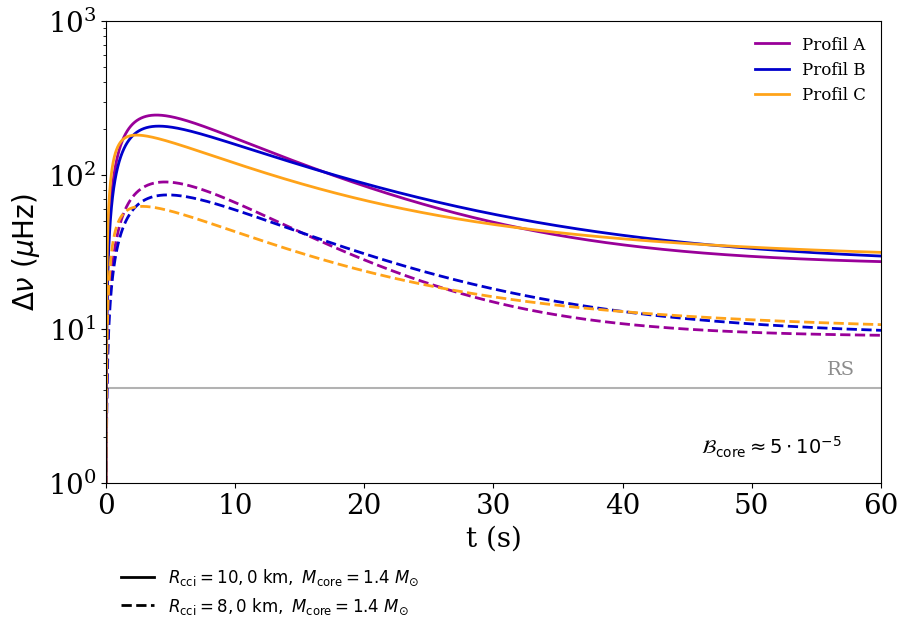
\includegraphics[width=0.9\textwidth]{../glitchrises-master/Exp1_Vary_R_run_1_R800000.0_M1.4.png}
    \caption{Simulace pro $R_{\rm cci} = 8$ km, fixní $M_{\rm core} = 1.4\,M_{\odot}$.}
    \label{fig:exp1_r8}
\end{figure}
\begin{figure}[!ht]
    \centering
    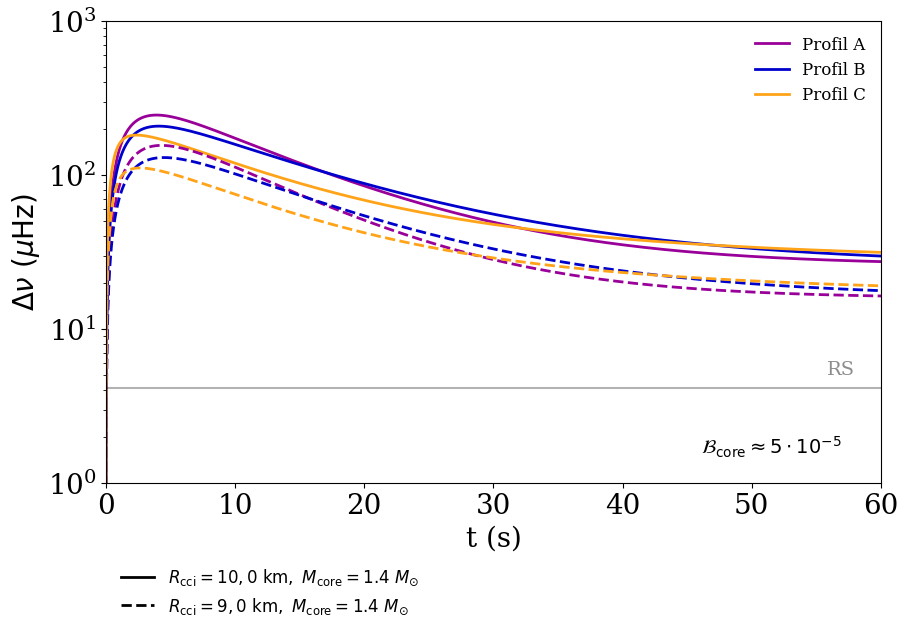
\includegraphics[width=0.9\textwidth]{../glitchrises-master/Exp1_Vary_R_run_2_R900000.0_M1.4.png}
    \caption{Simulace pro $R_{\rm cci} = 9$ km, fixní $M_{\rm core} = 1.4\,M_{\odot}$.}
    \label{fig:exp1_r9}
\end{figure}
\begin{figure}[!ht]
    \centering
    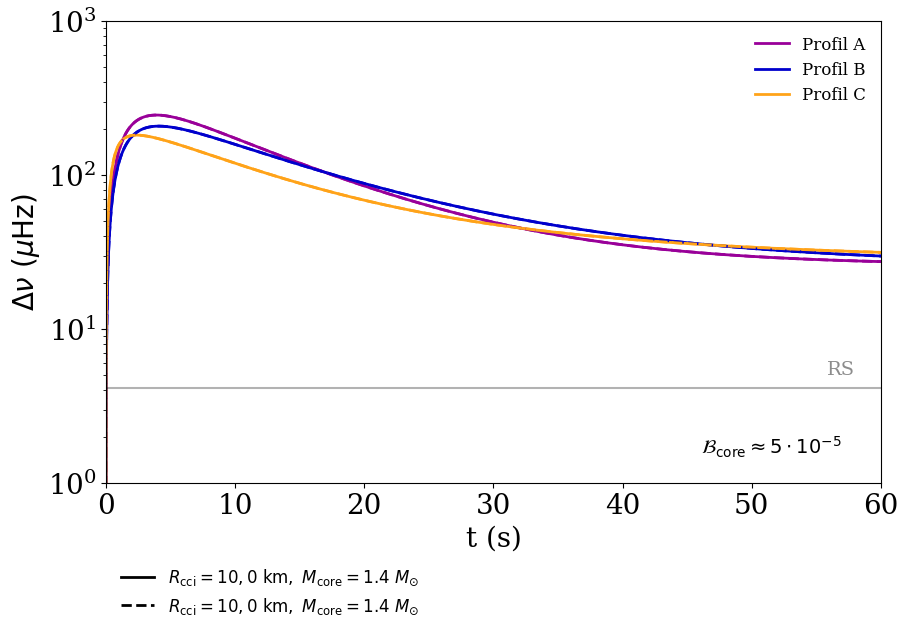
\includegraphics[width=0.9\textwidth]{../glitchrises-master/Exp1_Vary_R_run_3_R1000000.0_M1.4.png}
    \caption{Simulace pro $R_{\rm cci} = 10$ km, fixní $M_{\rm core} = 1.4\,M_{\odot}$.}
    \label{fig:exp1_r10}
\end{figure}
\begin{figure}[!ht]
    \centering
    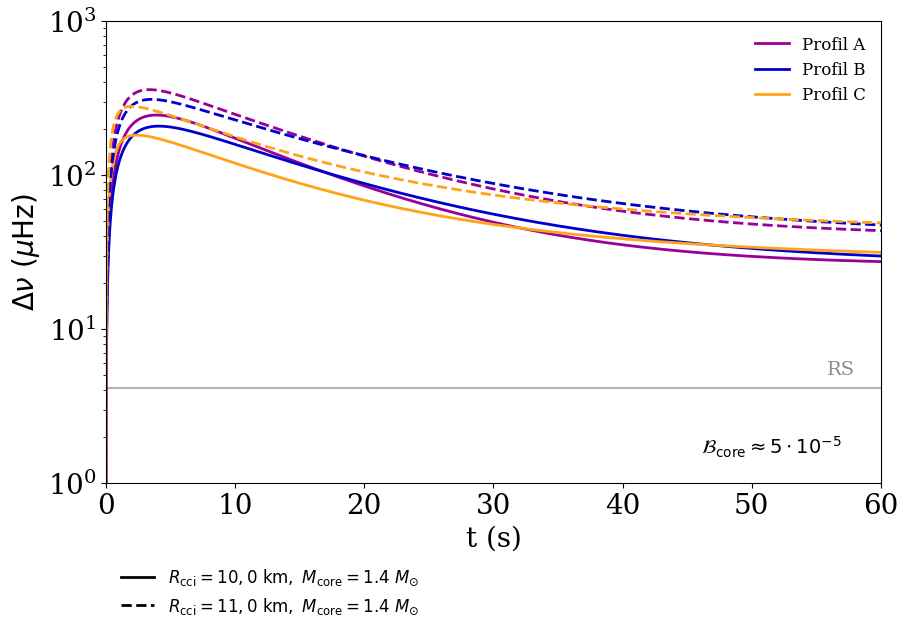
\includegraphics[width=0.9\textwidth]{../glitchrises-master/Exp1_Vary_R_run_4_R1100000.0_M1.4.png}
    
    \caption{Simulace pro $R_{\rm cci} = 11$ km, fixní $M_{\rm core} = 1.4\,M_{\odot}$.}
    \label{fig:exp1_r11}
\end{figure}
\begin{figure}[!ht]
    \centering
    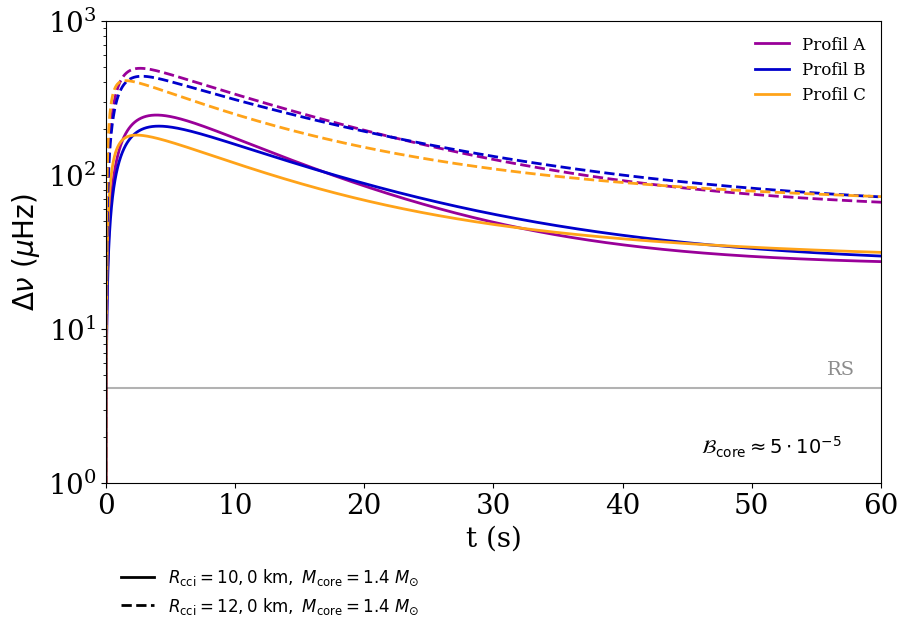
\includegraphics[width=0.9\textwidth]{../glitchrises-master/Exp1_Vary_R_run_5_R1200000.0_M1.4.png}
    \caption{Simulace pro $R_{\rm cci} = 12$ km, fixní $M_{\rm core} = 1.4\,M_{\odot}$.}
    \label{fig:exp1_r12}
\end{figure}
\begin{figure}[!ht]
    \centering
    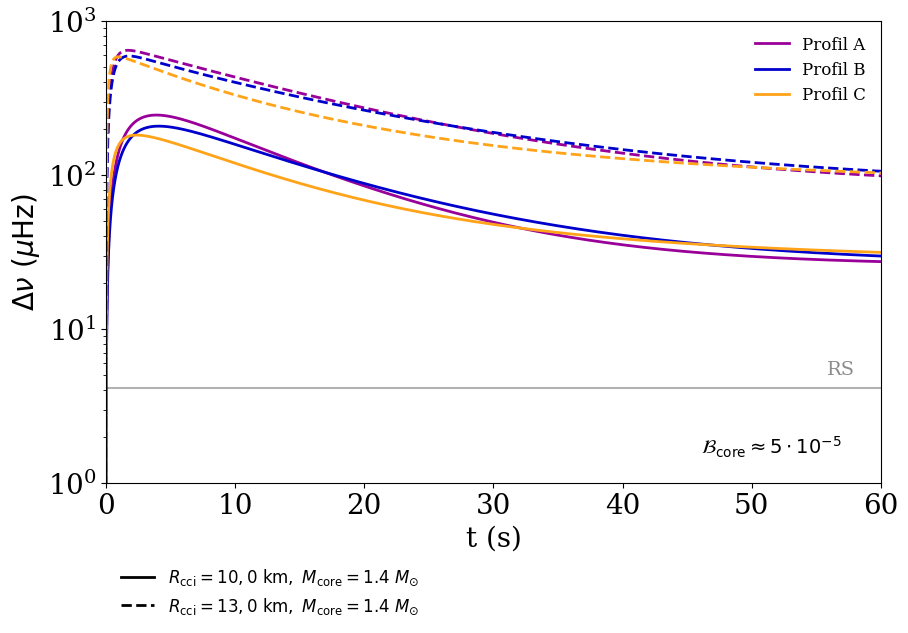
\includegraphics[width=0.9\textwidth]{../glitchrises-master/Exp1_Vary_R_run_6_R1300000.0_M1.4.png}
    \caption{Simulace pro $R_{\rm cci} = 13$ km, fixní $M_{\rm core} = 1.4\,M_{\odot}$.}
    \label{fig:exp1_r13}
\end{figure}
\begin{figure}[!ht]
    \centering
    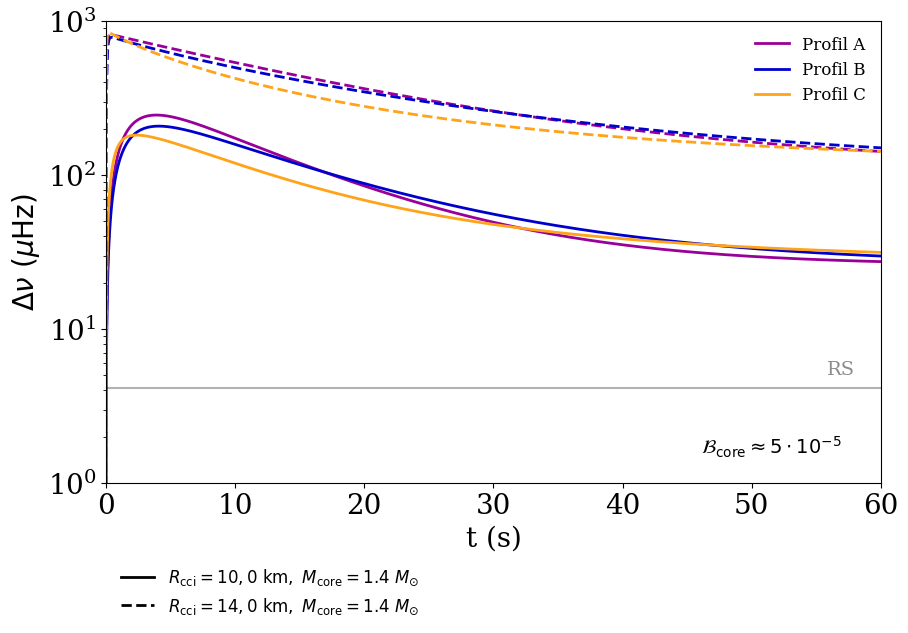
\includegraphics[width=0.9\textwidth]{../glitchrises-master/Exp1_Vary_R_run_7_R1400000.0_M1.4.png}
    \caption{Simulace pro $R_{\rm cci} = 14$ km, fixní $M_{\rm core} = 1.4\,M_{\odot}$.}
    \label{fig:exp1_r14}
\end{figure}

\clearpage
\subsection{Diskuze}
Ve výše zobrazených grafech pozorujeme náběh glitche (zrychlení frekvence rotace neutronové hvězdy) a jeho vývoj v krátkém časovém horizontu. Můžeme pozorovat, že frekvence rotace rychle naroste a následně se pomalu vrací k původnímu, pomalejšímu tempu rotace.
V první sérii grafů jsme zafixovali hmotnost jádra $M_{\rm core} = 1.4\ {\rm M}_{\odot}$ a zkoumali vliv poloměru rozhraní kůry a jádra $R_{\rm cci}$.
Pozorujeme, že čím větší $R_{\rm cci}$ je, tím větší je zrychlení rotace, a zároveň maximum frekvence rotace nastává dříve. 
Když zvětšíme $R_{\rm cci}$ a necháme $M_{\rm NS}$ konstantní, zvětší se i velikost kůry a zvětší se i jádro. Tím, že se hmotnost nezmění, látka nebude tak koncentrovaná a centrální hustota bude menší. Změna vnitřní struktury má vliv na rotační dynamiku. V objemnější kůře se nachází větší množství supratekutých neutron§. Tím roste moment setrvačnosti této supratekuté složky. V jádře se také zvyšuje moment setrvačnosti, ale ne tak výrazně jako v kůře. Proto pozorujeme strmější náběh glitche (s jádrem to více škubne).




\section{Závislost na hmotnosti jádra $M_{\rm core}$}
Zde je zobrazen vliv proměnlivé hmotnosti jádra při fixním poloměru kůry $R_{\rm cci} = 10\ {\rm km}$.

\begin{table}[htbp]
\centering
\caption{Výsledky simulace pro fixní $R_{\rm cci} = 10$ km a proměnnou hmotnost jádra $M_{\rm core}$.}
\label{tab:exp2_mcoeff}
\newsavebox{\tabletwobox}
\sbox{\tabletwobox}{\resizebox{\textwidth}{!}{%
\begin{tabular}{|c|c|c|c|c|c|c|c|c|c|}
\hline
$R_{\rm cci}$ & $M_{\rm core}$ & $M_{\rm NS}$ & $R_{\rm NS}$ & $A_{\rm max}$ & $t_{A_{\rm max}}$ & $B_{\rm max}$ & $t_{B_{\rm max}}$ & $C_{\rm max}$ & $t_{C_{\rm max}}$ \\ \relax
[km] & [$M_{\odot}$] & [$M_{\odot}$] & [km] & [$\mu$Hz] & [s] & [$\mu$Hz] & [s] & [$\mu$Hz] & [s] \\
\hline
10 & 1.1 & 1.12 & 11.188 & 416.22 & 3.06 & 364.6 & 3.19 & 335.05 & 1.79 \\
10 & 1.3 & 1.315 & 10.9 & 291.39 & 3.69 & 249.07 & 3.86 & 220.64 & 2.22 \\
10 & 1.5 & 1.512 & 10.694 & 207.39 & 4.07 & 174.45 & 4.27 & 151.02 & 2.49 \\
10 & 1.7 & 1.709 & 10.542 & 149.15 & 4.33 & 124.07 & 4.54 & 105.76 & 2.66 \\
10 & 1.9 & 1.907 & 10.423 & 107.75 & 4.5 & 88.91 & 4.72 & 74.97 & 2.79 \\
10 & 2 & 2.006 & 10.373 & 91.55 & 4.56 & 75.3 & 4.79 & 63.22 & 2.84 \\
10 & 2.2 & 2.205 & 10.288 & 65.73 & 4.66 & 53.78 & 4.9 & 44.83 & 2.91 \\
\hline
\end{tabular}%
}
}
\resizebox{\textwidth}{!}{\usebox{\tabletwobox}}
\end{table}

\begin{figure}[htbp]
    \centering
    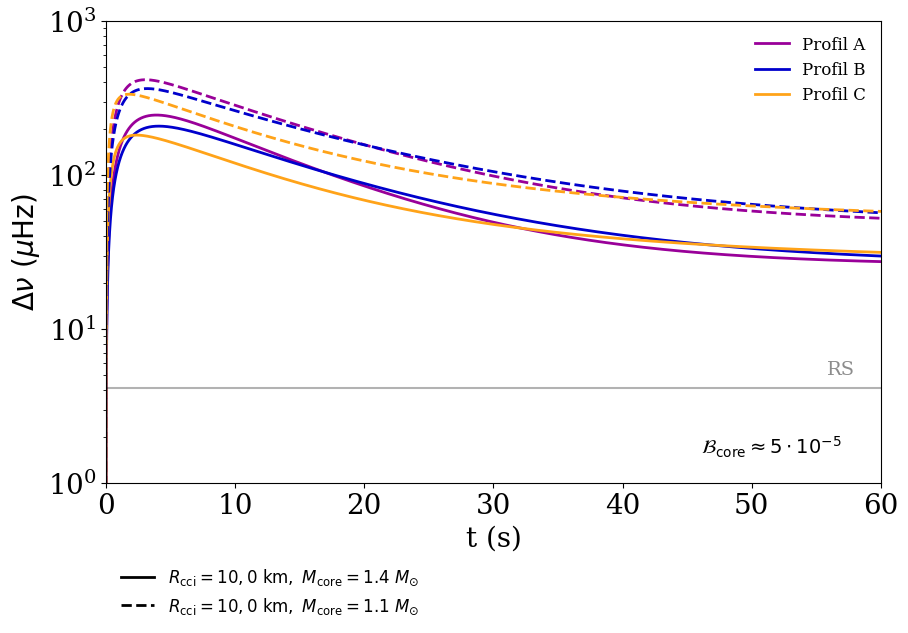
\includegraphics[width=0.9\textwidth]{../glitchrises-master/Exp2_Vary_M_run_1_R1000000_M1.1.png}
    \caption{Simulace pro $M_{\rm core} = 1.1\,M_{\odot}$, fixní $R_{\rm cci} = 10\,{\rm km}$.}
    \label{fig:exp2_m11}
\end{figure}
\begin{figure}[htbp]
    \centering
    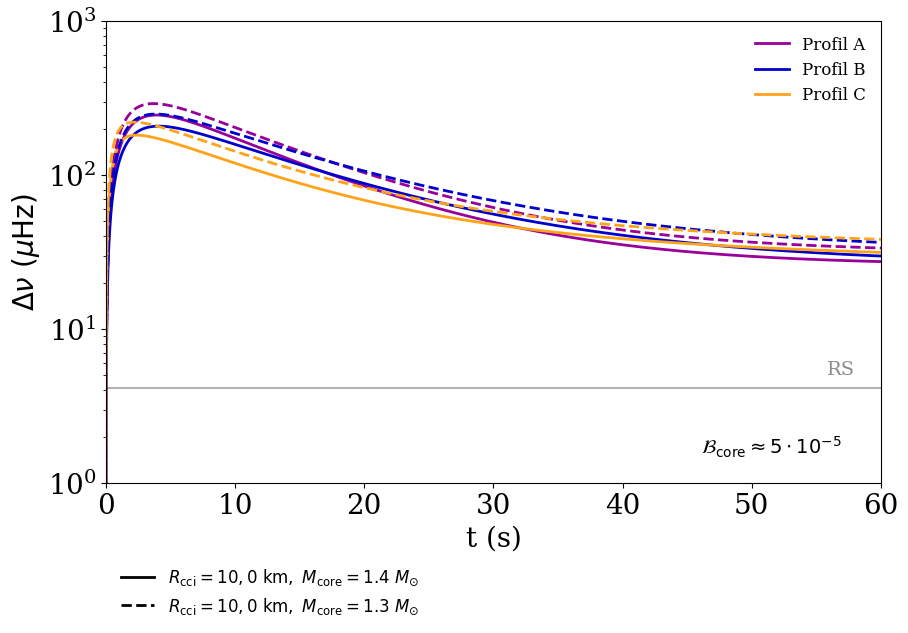
\includegraphics[width=0.9\textwidth]{../glitchrises-master/Exp2_Vary_M_run_2_R1000000_M1.3.png}
    \caption{Simulace pro $M_{\rm core} = 1.3\,M_{\odot}$, fixní $R_{\rm cci} = 10\,{\rm km}$.}
    \label{fig:exp2_m13}
\end{figure}
\begin{figure}[htbp]
    \centering
    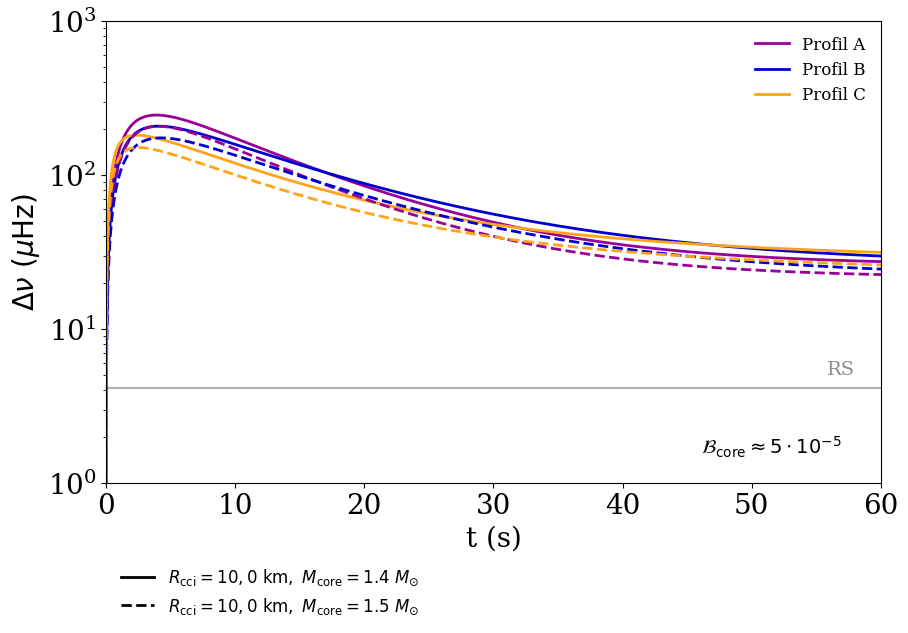
\includegraphics[width=0.9\textwidth]{../glitchrises-master/Exp2_Vary_M_run_3_R1000000_M1.5.png}
    \caption{Simulace pro $M_{\rm core} = 1.5\,M_{\odot}$, fixní $R_{\rm cci} = 10\,{\rm km}$.}
    \label{fig:exp2_m15}
\end{figure}
\begin{figure}[htbp]
    \centering
    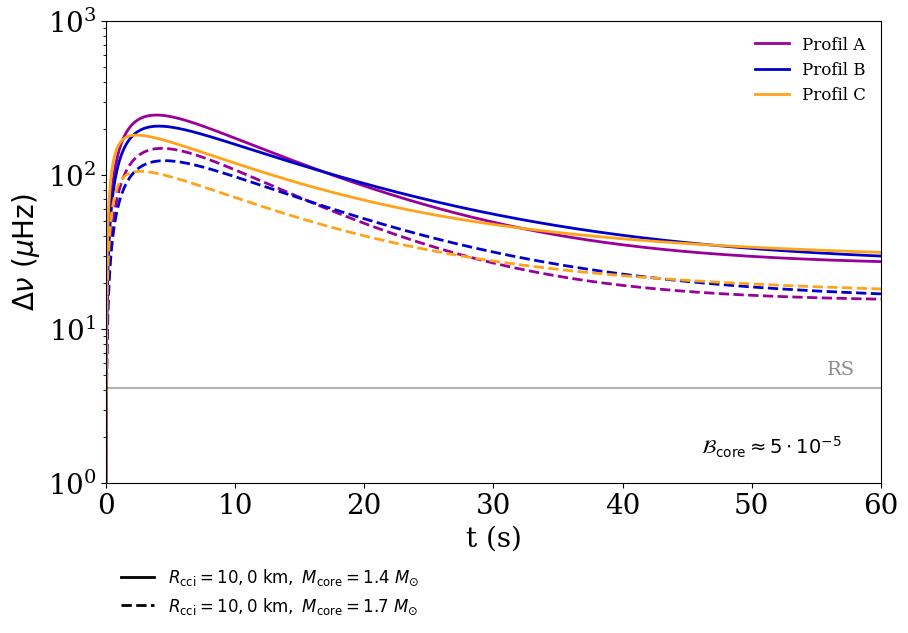
\includegraphics[width=0.9\textwidth]{../glitchrises-master/Exp2_Vary_M_run_4_R1000000_M1.7.png}
    \caption{Simulace pro $M_{\rm core} = 1.7\,M_{\odot}$, fixní $R_{\rm cci} = 10\,{\rm km}$.}
    \label{fig:exp2_m17}
\end{figure}
\begin{figure}[htbp]
    \centering
    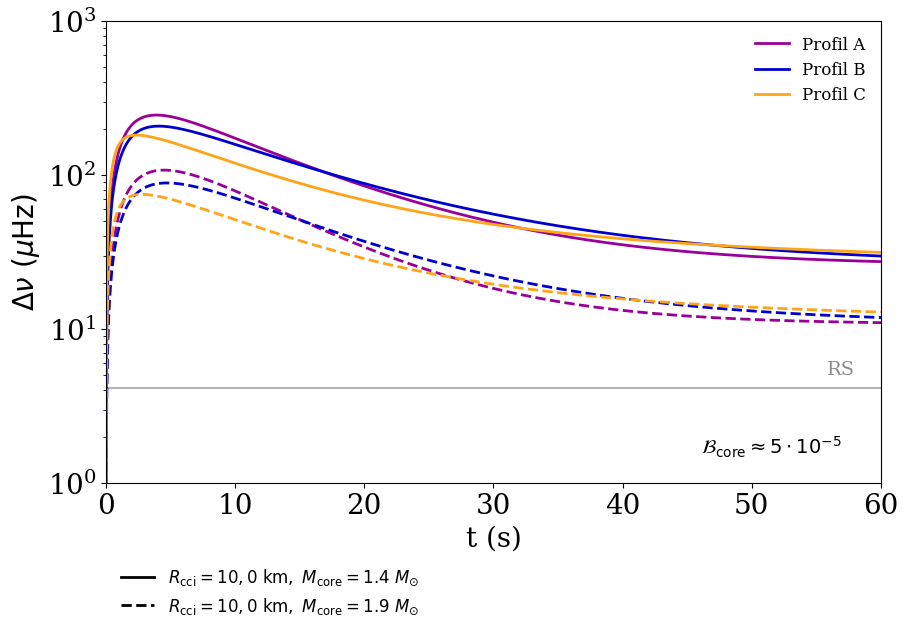
\includegraphics[width=0.9\textwidth]{../glitchrises-master/Exp2_Vary_M_run_5_R1000000_M1.9.png}
    \caption{Simulace pro $M_{\rm core} = 1.9\,M_{\odot}$, fixní $R_{\rm cci} = 10\,{\rm km}$.}
    \label{fig:exp2_m19}
\end{figure}
\begin{figure}[htbp]
    \centering
    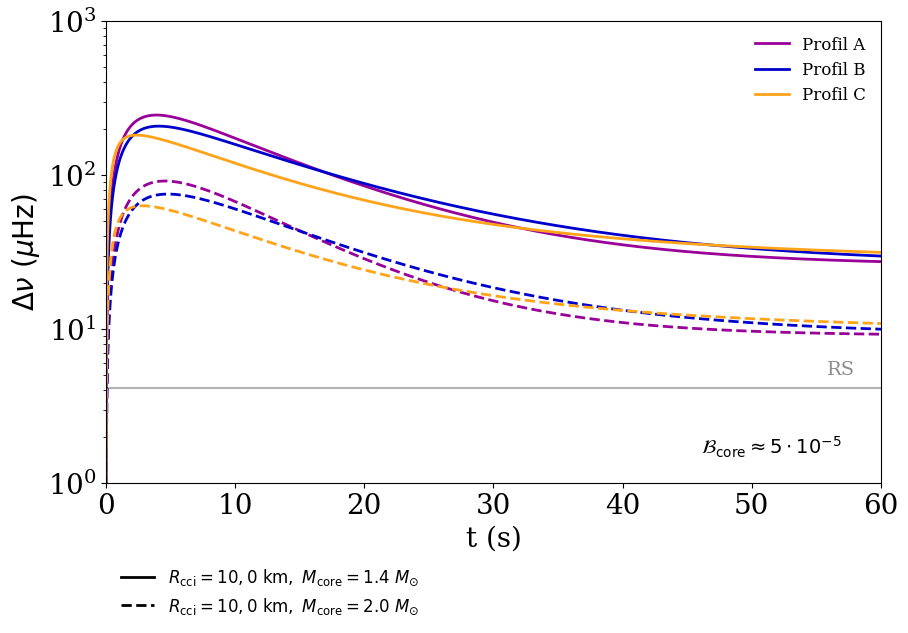
\includegraphics[width=0.9\textwidth]{../glitchrises-master/Exp2_Vary_M_run_6_R1000000_M2.0.png}
    \caption{Simulace pro $M_{\rm core} = 2.0\,M_{\odot}$, fixní $R_{\rm cci} = 10\,{\rm km}$.}
    \label{fig:exp2_m20}
\end{figure}
\begin{figure}[htbp]
    \centering
    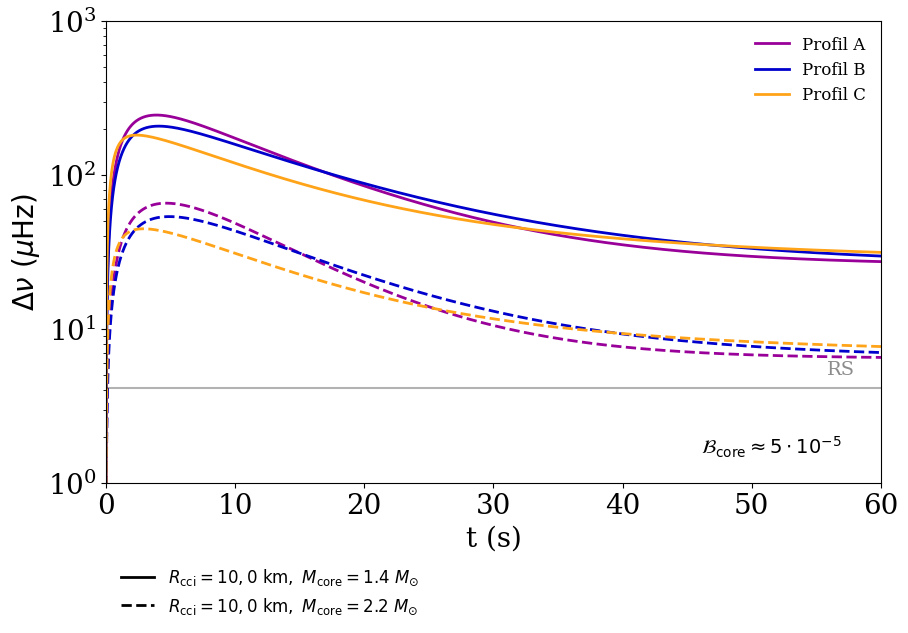
\includegraphics[width=0.9\textwidth]{../glitchrises-master/Exp2_Vary_M_run_7_R1000000_M2.2.png}
    \caption{Simulace pro $M_{\rm core} = 2.2\,M_{\odot}$, fixní $R_{\rm cci} = 10\,{\rm km}$.}
    \label{fig:exp2_m22}
\end{figure}


\subsection{Diskuze}
Když zvětším hmotnost neutronové hvězdy $M_{\rm NS}$, zvětší se gravitace a zvětší se také tlak a hustota. Kvůli tomu bude jádro neutronové hvězdy větší a kůra tenčí. Čím je kůra tenčí, tím má menší moment setrvačnosti, a tím i celkové množství supratekutých neutronů je menší. Proto pozorujeme menší zrychlení frekvence rotace a tím i pomalejší náběh glitche.



\section{Shrnutí maxim – Profil A}
Následující párové grafy znázorňují souhrnné trendy závislosti absolutní výšky frekvenčního skoku ($\Delta\nu_{\rm max}$) a času dosažení tohoto maxima ($t_{\rm max}$) na zkoumaných parametrech. Plným červeným křížkem je pro jasné srovnání vyznačena referenční Sada 1 s nominálními parametry $R_{\rm cci} = 10\ {\rm km}$ a $M_{\rm core} = 1.4\ M_{\odot}$.


\begin{figure}[htbp]
    \centering
    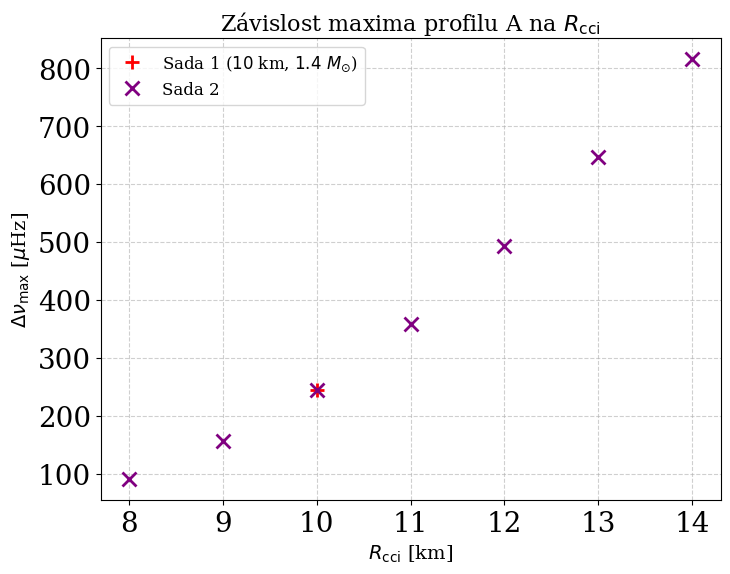
\includegraphics[width=0.48\textwidth]{../glitchrises-master/zavislost_maxA_Rcci.png}
    \hfill
    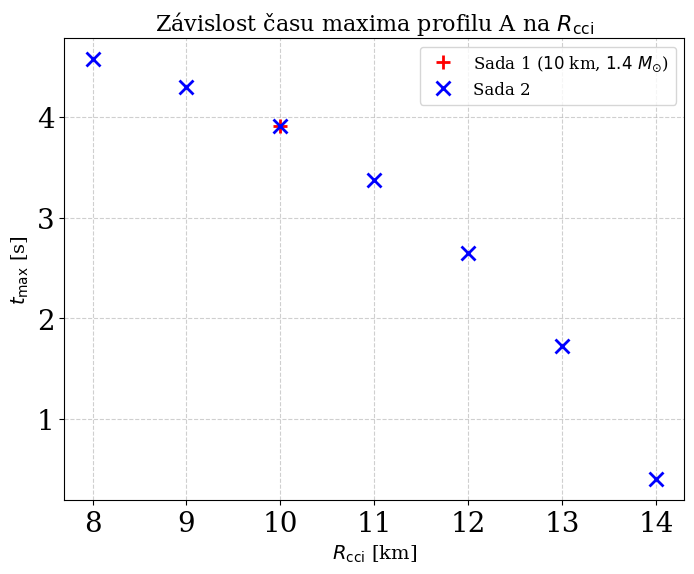
\includegraphics[width=0.48\textwidth]{../glitchrises-master/zavislost_casA_Rcci.png}
    \caption{Závislost maxima a času maxima profilu A na poloměru rozhraní $R_{\rm cci}$.}
    \label{fig:dep_rcci}
\end{figure}

\begin{figure}[htbp]
    \centering
    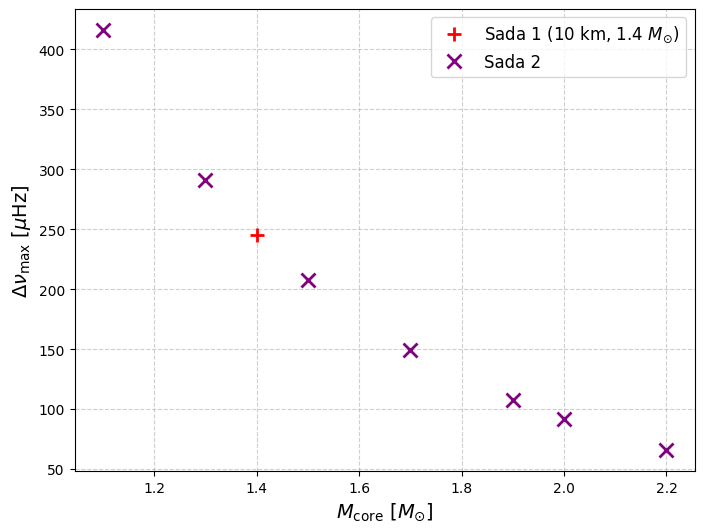
\includegraphics[width=0.48\textwidth]{../glitchrises-master/zavislost_maxA_Mcoeff.png}
    \hfill
    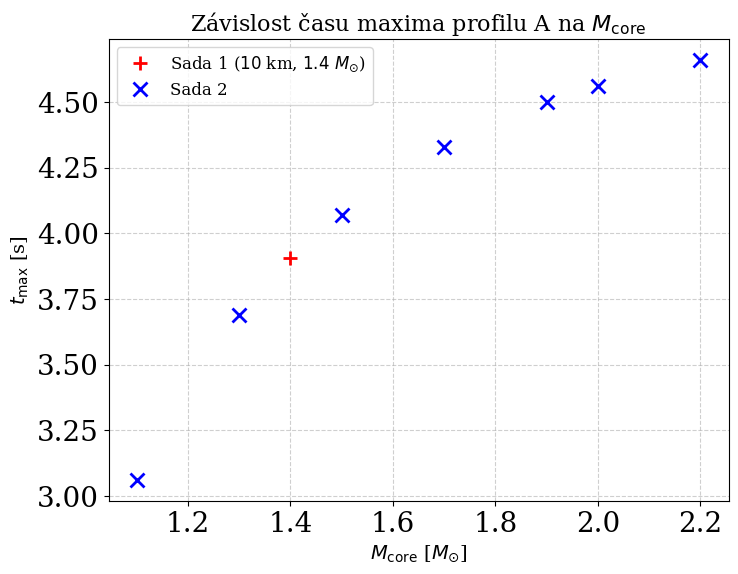
\includegraphics[width=0.48\textwidth]{../glitchrises-master/zavislost_casA_Mcoeff.png}
    \caption{Závislost maxima a času maxima profilu A na hmotnosti $M_{\rm core}$.}
    \label{fig:dep_mcoeff}
\end{figure}


\subsection{Diskuze}
První grafy znázorňují závislost maximální frekvence profilu A na poloměru rozhraní $R_{\rm cci}$. S rostoucím $R_{\rm cci}$ je větší i kůra. Čím je větší kůra, tím je větší "zásoba" momentu hybnosti, a pak je větší i maximum glitche.

Druhý graf znázorňuje závislost času maxima frekvence na $R_{\rm cci}$. I zde platí, že s rostoucím $R_{\rm cci}$ rostě i velikost kůry. Čím větší kůra, tím větší množství superfluidních neutronů. Čím více těchto superfluidních neutronů v kůře máme, tím rychleji naběhne glitch, tedy $\Delta t$ bude menší.

Třetí graf znázorňuje závislost maximální frekvence profilu A na hmotnosti $M_{\rm core}$.
S rostoucím $M_{\rm core}$ se zmenšuje poloměr kůry $R_{\rm cci}$, a tím pádem se zmenšuje i množství superfluidních neutronů. Zmenšením množství superfluidních neutronů se glitche naběhne pomaleji a tím pádem je i maximum glitche menší.

Ve čtvrtém grafu vidíme závislost času maxima frekvence na $M_{\rm core}$. Menší kůra zapříčiní menší množství superfluidních neutronů, které ovlivňují rychlost náběhu glitche. Proto se nám glitche naběhne pomaleji, tedy $\Delta t$ je s rostoucím $M_{\rm core}$ větší.
  
\section{Diskuse a interpretace výsledků}


\newpage

\chapter{Závěr}





%%%%%%%%%%%%%%%%%%%%%%%%%%%%%%%%%%%%%%%%%%%%%%%%%%%%%%%%%%%%%%%%%%
%% Závěrečnou práci lze strukturovat do částí (parts, úroveň -1,
%% nevyžadováno, ale obvykle výhodné), zatímco kapitoly (úroveň 0)
%% jsou průběžně číslovány od 1.

%%%%%%%%%%%%%%%%%%%%%%%%%%%%%%%%%%%%%%%%%%%%%%%%%%%%%%%%%%%%%%%%%%
%% Zde začíná první část. Všimněte si, jak strukturální příkazy
%% (a mnohé další čítače generující příkazy) jsou opatřeny
%% unikátními jmény. To se může hodit pro budoucí křížové odkazy:

%\part{Postupy a řešení}\label{procsol}

%%%%%%%%%%%%%%%%%%%%%%%%%%%%%%%%%%%%%%%%%%%%%%%%%%%%%%%%%%%%%%%%%%%
%% Toto je inkludovaný LaTeXový soubor `cp_inst.tex'.           %%
%% ------------------------------------------------------------ %%
%% Verze 2022-05-23                                             %%
%% Vyvíjí & udržuje <stanislav.hledik@physics.slu.cz>           %%
%%%%%%%%%%%%%%%%%%%%%%%%%%%%%%%%%%%%%%%%%%%%%%%%%%%%%%%%%%%%%%%%%%

\chapter{Instalace}\label{install}%%%%%%%%%%%%%%%%%%%%%%%%%%%%%%%%%%%%%%%%%

\section{Získání balíčku \ipotname{}}\label{instgetpack}%%%%%%%%%%%%%%%%%%%

Domovská stránka balíčku \pkg{\ipotname} je \theshome, sekce \TeX. Můžete se
rozhodnout pro jeden z~následujících způsobů instalace: \uv{vše v~jednom} nebo
\uv{zdrojové texty a knihovny odděleně}. Ke stažení pro vás vhodné varianty
využijte odkazů v~textu níže. Kontrolní součty jsou v~souboru
\href{https://is.slu.cz/www/hle0002/vyuka/aid/ipothes/CHECKSUMS.md5}%
{\pgm{CHECKSUMS.md5}}.

\section{Instalace \uv{vše v~jednom}}\label{installinone}%%%%%%%%%%%%%%%%%%

Stáhněte si archiv
\href{https://is.slu.cz/www/hle0002/vyuka/aid/ipothes/vzorova\_prace.ipothes.zip}%
{\pgm{\thesnamecze .\ipotname .zip}} obsahující ve společném adresáři
\pgm{manual} po rozbalení kromě nezbytných \LaTeX ových
knihoven\footnote{Dokumentní třída, bibliografický styl, lokalizační soubory a
  systémové obrázky s~fiktivním zadáním a aktuálně se znaky Fyzikálního ústavu
  v~Opavě, Fi\-lo\-zo\-fic\-ko-pří\-ro\-do\-vě\-dec\-ké fakulty v~Opavě a
  Matematického ústavu v~Opavě.} také zdrojové soubory nutné pro kompilaci
tohoto hypertextového českého manuálu
\href{https://is.slu.cz/www/hle0002/vyuka/aid/ipothes/vzorova\_prace.pdf}%
{\pgm{\thesnamecze .pdf}}.\footnote{Není součástí výše uvedeného archivu, jenž
  neobsahuje výstupy ani intermediální soubory \pgm{*.aux}, \pgm{*.log},
  \pgm{*.toc}, \pgm{*.lof}, \pgm{*.lot}, \pgm{*.out}, \pgm{*.bbl},
  \pgm{*.blg}, \pgm{*.idx}, \pgm{*.ind}, \pgm{*.ilg}.} Tuto možnost nejspíše
zvolí uživatelé, kteří zamýšlejí využít \pkg{\ipotname} pouze pro jednorázové
napsání závěrečné práce a nechtějí si jím \uv{kontaminovat} svůj \TeX{}
systém. Je rovněž určena pro uživatele cloudového systému
Overleaf~\cite{Ovr:LIVE::Overleaf}.\footnote{Výhodou je také, že po dokončení
  práce a archivování se uchovají pohromadě zdrojové texty i~\LaTeX ové
  knihovny (jež budou pravděpodobně vyvíjeny bez záruky zpětné kompatibility),
  takže kompatibilita je víceméně zachována. Nevýhodou je vyšší míra chaosu ve
  vašem pracovním adresáři.}

Váš \TeX{} systém není třeba v~tomto případě nijak konfigurovat, všechny
soubory budou nalezeny. V~pracovním adresáři \pgm{manual} (klidně si jej
přejmenujte) si vytvořte nový vlastní hlavní \LaTeX ový soubor a případně
i~inkludované soubory \pgm{include/*.tex} podle ukázkového hlavního \LaTeX
ového souboru \pgm{\thesnamecze .tex}\footnote{Velmi doporučujeme, aby
  v~názvech vašich zdrojových souborů ani v~cestách k~nim nebyly znaky
  s~diakritikou a mezery. Ušetříte si tím možná nepříjemná překvapení.} nebo
pokračujte formou přejmenovávání a editace obsahu zdrojáků tohoto manuálu.

\section{Instalace \uv{zdrojové texty a knihovny odděleně}}\label{instsepar}%%

Stáhněte si archivy

\begin{enumerate}
\item \href{https://is.slu.cz/www/hle0002/vyuka/aid/ipothes/ipothes.tds.zip}%
  {\pgm{\ipotname .tds.zip}} obsahující pouze knihovní
  soubory\footnote{Dokumentní třída, bibliografický styl, dokumentační
    soubory, lokalizační soubory a systémové obrázky s~fiktivním zadáním a
    aktuálně se znaky Fyzikálního ústavu v~Opavě,
    Fi\-lo\-zo\-fic\-ko-pří\-ro\-do\-vě\-dec\-ké fakulty v~Opavě a
    Matematického ústavu v~Opavě.} uložené v~kanonické adresářové struktuře
  požadované systémem \TeX~\cite{Sch:LIVE::TDS}, a to v~adresářích
  \pgm{bibtex}, \pgm{doc} a \pgm{tex} a struktuře pod nimi;
\item
  \href{https://is.slu.cz/www/hle0002/vyuka/aid/ipothes/vzorova\_prace.zip}%
  {\pgm{\thesnamecze .zip}} obsahující v~adresáři \pgm{manual} pouze zdrojové
  soubory nutné ke kompilaci tohoto českého manuálu
  \href{https://is.slu.cz/www/hle0002/vyuka/aid/ipothes/vzorova\_prace.pdf}%
  {\pgm{\thesnamecze .pdf}}.\footnote{Není součástí výše uvedeného archivu,
    jenž neobsahuje výstupy ani intermediální soubory \pgm{*.aux},
    \pgm{*.log}, \pgm{*.toc}, \pgm{*.lof}, \pgm{*.lot}, \pgm{*.out},
    \pgm{*.bbl}, \pgm{*.blg}, \pgm{*.idx}, \pgm{*.ind}, \pgm{*.ilg}.}
\end{enumerate}

\noindent
Tato možnost je vhodná pro ty uživatele, kteří si chtějí integrovat balíček
\pkg{\ipotname} do svého \TeX{} systému, takže jej budou moci využívat pro
více projektů.

\begin{figure}[p]
\setlength{\fboxsep}{0sp}
\begin{center}
\fbox{
\includegraphics[width=.86\linewidth]{MiKTeXdirs}}
\end{center}
\caption[Přidání adresáře do cest \distroMiKTeX u]%
{\label{MiKTeXdirs}Přidání adresáře do cest distribuce \distroMiKTeX .}
\end{figure}

\begin{figure}[p]
\setlength{\fboxsep}{0sp}
\begin{center}
\fbox{
\includegraphics[width=.86\linewidth]{TeXLiveInstaller1}}
\end{center}
\caption[Přidání adresáře do cest \distroTeXLive]%
{\label{TeXLivedirs}Přidání adresáře do cest distribuce \distroTeXLive{} (TEXMFHOME).}
\end{figure}

Integraci provedete rozbalením prvního archivu včetně celých adresářových
stromů do libovolného adresáře,\footnote{Název a cesta opět bez znaků
  s~diakritikou a mezer.}  který následně pomocí konsole vašeho \TeX{} systému
přidáte do databáze prohledávaných cest. Kupříkladu v~konsoli distribuce
\distroMiKTeX~\cite{Sch:LIVE::MiKTeX} použijete postup znázorněný na
obrázku~\ref{MiKTeXdirs}, v~instalátoru distribuce
\distroTeXLive~\cite{TUG:LIVE::TeXLive} použijete postup znázorněný na
obrázku~\ref{TeXLivedirs}, přičemž obsah archivu byl v~obou případech rozbalen
to prázdného adresáře \pgm{texmf}. Po přidání cesty je třeba aktualizovat
databázi prohledávaných cest; příklad tohoto kroku v~\distroMiKTeX u je na
obrázku~\ref{MiKTeXrefr}, v~\distroTeXLive{} na obrázku~\ref{TeXLiverefr}.

\begin{figure}[p]
\setlength{\fboxsep}{0sp}
\begin{center}
\fbox{
\includegraphics[width=.82\linewidth]{MiKTeXrefr}}
\end{center}
\caption[Aktualizace databáze cest \distroMiKTeX u]%
{\label{MiKTeXrefr}Aktualizace databáze cest distribuce \distroMiKTeX .}
\end{figure}

\begin{figure}[p]
\setlength{\fboxsep}{0sp}
\begin{center}
\fbox{
\includegraphics[width=.82\linewidth]{TeXLiveShell}}
\end{center}
\caption[Aktualizace databáze cest \distroTeXLive]%
{\label{TeXLiverefr}Aktualizace databáze cest distribuce \distroTeXLive .}
\end{figure}

Alternativní možností je rozbalení prvního archivu včetně celých adresářových
stromů do některého ze systémových adresářů vaší instalace \TeX
u.\footnote{V~\distroMiKTeX u např. do \pgm{c:\textbackslash
    Users\textbackslash username\textbackslash AppData\textbackslash
    Roaming\textbackslash MiKTeX}.}  Takový adresář není třeba přidávat do
databáze prohledávaných cest (již v~ní je), opět je však třeba aktualizovat
databázi prohledávaných cest podle obrázku~\ref{MiKTeXrefr}
nebo~\ref{TeXLiverefr}.

S~obsahem druhého archivu, \pgm{\thesnamecze .zip}, pak naložíte způsobem
analogickým jako v~Sekci~\ref{installinone}. Nebude již obsahovat nepřehledné
množství systémových souborů, funkčnost však bude identická.

\section{Testování}\label{insttest}%%%%%%%%%%%%%%%%%%%%%%%%%%%%%%%%%%%%%%%%

Po instalaci libovolným z~obou výše popsaných způsobů doporučujeme otestovat
funkčnost balíčku \pkg{\ipotname} v~\TeX{} systému na vašem počítači
následovně. Aniž byste na zdrojových textech či názvech adresářů cokoli
měnili, přemístěte se do adresáře s~fiktivní závěrečnou prací \pgm{manual} a
proveďte kompilaci pomocí formátu pdf\LaTeX, poté zformátujte bibliografii
pomocí \BibTeX u, a nakonec kompilujte pdf\LaTeX em tolikrát, dokud z~logu
nezmizí hlášky typu\footnote{Jsou-li příkazy \pgm{\textbackslash cite}
  přítomny přímo v~bibliografických položkách v~\pgm{*.bib} souborech, což je
  případ tohoto manuálu, je zapotřebí dokonce dvojí zpracování \BibTeX em:
  nejprve pdf\LaTeX, poté \BibTeX, pdf\LaTeX, opět \BibTeX, a pdf\LaTeX{}
  tolikrát, dokud nezmizí uvedené hlášky.}

{\small
\begin{verbatim}
Package natbib Warning: There were undefined citations.
Package natbib Warning: Citation(s) may have changed.
(natbib)                Rerun to get citations correct.
LaTeX Warning: There were undefined references.
LaTeX Warning: Label(s) may have changed.
               Rerun to get cross-references right.
\end{verbatim}
\par}

Mějte na paměti, že některá IDE jako např. TeXworks distribuovaný jako součást
\distroMiKTeX u mají implicitně nastavenu kompilaci
pdf\LaTeX${}+{}$\MakeIndex${}+{}$\BibTeX; toto je třeba změnit na kompilaci
pouze pdf\LaTeX em a \BibTeX em podle obrázku~\ref{TeXworksCompile}: nechceme
aktualizovat soubor s~vytvořeným rejstříkem \pgm{\thesnamecze .ind} a
spouštění pomocného programu \MakeIndex{} je zbytečné. Uživatelé linuxového
shellu~\cite{Sie:1999:LinuxNutshell:} mohou kompilovat pomocí příkazového
řádku jako na obrázku~\ref{BashCompile}.

\begin{figure}[t]
\setlength{\fboxsep}{0sp}
\begin{minipage}{.48\linewidth}
\begin{center}
\fbox{
\includegraphics[width=0.99\linewidth]{TeXworks_pdfLaTeX}}
\end{center}
\end{minipage}\hfill%
\begin{minipage}{.48\linewidth}
\begin{center}
\fbox{
\includegraphics[width=0.99\linewidth]{TeXworks_TypesetMenu}}
\end{center}
\end{minipage}
\caption[Nastavení testovací kompilace v~IDE TeXworks]%
{\label{TeXworksCompile}Nastavení testovací kompilace v~integrovaném vývojovém
  prostředí TeXworks z~distribuce \distroMiKTeX .}
\end{figure}
\begin{figure}[t]
{\small
\begin{verbatim}
$ c=pdflatex; i=vzorova_prace; $c $i; bibtex $i; $c $i; $c $i
\end{verbatim}
\par}
\caption[Testovací kompilace v~bash]%
{\label{BashCompile}Testovací kompilace v~shellu \pkg{bash}. Počet běhů
  pdf\LaTeX u (\pgm{\$c \$i}) po sestavení bibliografie může být v~případě
  potřeby zvýšen.}
\end{figure}

Kompilace by měla proběhnout bez chyb, pochopitelně po \emph{on the fly}
doinstalaci chybějících požadovaných balíčků při první kompilaci, jak to dělá
např. distribuce \distroMiKTeX~\cite{Sch:LIVE::MiKTeX} (což může trvat nějaký
čas). Jejím výsledkem by měl být hypertextový \designation{pdf} soubor
\pgm{\thesnamecze .pdf} obsahově shodný s~tímto manuálem ve formě fiktivní
závěrečné práce.\footnote{Velikost se může lišit podle nastavené komprese
  \designation{pdf}.}

Proběhla-li kompilace bez chyb, lze bez obav začít používat balíček
\pkg{\ipotname} pro přípravu vlastní práce.

Pokud nic z~výše uvedeného nefunguje, kontaktujte lokálního \TeX ového wizarda
nebo se obraťe o~radu na \url{https://tex.stackexchange.com/} resp.
\url{https://stackoverflow.com/questions/tagged/latex}.

\section{Copyright}\label{copyright}%%%%%%%%%%%%%%%%%%%%%%%%%%%%%%%%%%%%%%%

Balíček \pkg{\ipotname} je freeware. Omezení: kýmkoli (kromě autora) provedená
jakákoli úprava nesmí být distribuována pod stejným jménem, včetně jmen
adresářů, souborů s~dokumentní třídou, bibliografickým stylem, a všech výskytů
retězce \pgm{"\ipotname "} v~nich a ve zdrojových, konfiguračních a ostatních
textových souborech knihovny a manuálu.

\endinput

%% 
%% End of file `cp_inst.tex'.

%%%%%%%%%%%%%%%%%%%%%%%%%%%%%%%%%%%%%%%%%%%%%%%%%%%%%%%%%%%%%%%%%%%
%% Toto je inkludovaný LaTeXový soubor `cp_pream.tex'.          %%
%% ------------------------------------------------------------ %%
%% Verze 2022-06-03                                             %%
%% Vyvíjí & udržuje <stanislav.hledik@physics.slu.cz>           %%
%%%%%%%%%%%%%%%%%%%%%%%%%%%%%%%%%%%%%%%%%%%%%%%%%%%%%%%%%%%%%%%%%%

\chapter{Preambule}\label{preamble}%%%%%%%%%%%%%%%%%%%%%%%%%%%%%%%%%%%%%%%%

Úvodní část \LaTeX ového hlavního zdrojového souboru nacházející se mezi
specifikací dokumentní třídy v~\pgm{\textbackslash
  documentclass[}$\langle$\emph{volby}$\rangle$\pgm{]\{\ipotname\}} a začátkem
prostředí \verb!\begin{document}! se nazývá
  \emph{preambule}~\cite{Ryb:2005:LaTeX:3}. Umisťují se do ní příkazy pro
  načítání balíčků pomocí příkazu \pgm{\textbackslash usepackage} a
  uživatelská nastavení, definice či redefinice. Po \verb!\begin{document}!
    následuje \emph{tělo dokumentu}, kam se zapisuje zejména vlastní text
s~potřebným kontextovým značkováním.

U~dokumentní třídy \pgm{\ipotname .cls} je doporučeno umisťovat do preambule
pouze načítání balíčků, avšak uživatelská nastavení, definice a redefinice
raději přesunout do konfiguračního souboru \pgm{\ipotname .cfg} popsaného
v~Dodatku~\ref{config}. Primárním důvodem tohoto doporučení je, že
konfigurační soubor \pgm{\ipotname .cfg} je načítán v~argumentu makra
\pgm{\textbackslash AtEndPreamble}~\cite{Wri-Leh:LIVE:CTAN:etoolbox} až po
balíčku \pkg{hyperref}, jenž sám redefinuje některé příkazy (viz
Dodatek~\ref{packages}). Sekundární důvod je víceméně estetický~-- sleduje
oddělení souboru s~konfigurací a souboru s~textem. Jinak ale lze vaše definice
a redefinice v~preambuli uvést, pokud si je otestujete.

Celý hlavní zdrojový soubor \pgm{\thesnamecze .tex} tohoto manuálu jakožto
česky psané fiktivní závěrečné práce je včetně preambule bohatě komentován.
Doporučujeme čtenáři tyto komentáře projít; ostatně vezme-li soubor
\pgm{\thesnamecze .tex} jako základ pro psaní vlastní práce, je četba
komentářů zcela dostačující. Níže uvedené fragmenty preambule jsou načteny
přímo z~\pgm{\thesnamecze .tex} pomocí balíčku
\pkg{fancyvrb}~\cite{Vos:LIVE:CTAN:fancyvrb}.

\section{Specifikace dokumentní třídy}\label{docclass}%%%%%%%%%%%%%%%%%%%%%

Preambuli samotné předchází zavedení dokumentní třídy \pgm{\ipotname .cls} a
nastavení jejích voleb, jež jsou popsány v~Dodatku~\ref{options}. Právě jedna
z~voleb \pgm{draft} nebo \pgm{final} musí zůstat odkomentovaná (nenechávajte
je obě zakomentované nebo odkomentované); ostatní voleb lze použít podle
vašich vlastních požadavků (implicitní chování při zakomentovaní volbě je
uvedeno v~závorce komentáře):

\VerbatimInput[frame=none,firstline=16,lastline=24,fontsize=\small]%
{vzorova_prace.tex}

\section{Fonty a jazyková lokalizace}\label{fontslang}%%%%%%%%%%%%%%%%%%%%%

Nyní začíná vlastní preambule. Pro zajištění vyšší flexibility nejsou
příslušné balíčky načítány v~dokumentní třídě (viz Dodatek~\ref{packages}),
ale až zde v~preambuli.

Balíčky načtené v~následujícím kódu způsobí globální použití nadrodiny fontů
Latin Modern (\pkg{lm}~\cite{Jac:LIVE:CTAN:lm}) místo nadrodiny fontů Computer
Modern (\pkg{cm}). Je nutné uvést kódování fontu volbou \opt{T1} balíčku
\pkg{fontenc}~\cite{LtX:LIVE:CTAN:fontenc} a kódování zdrojových textů volbou
\opt{utf8} balíčku \pkg{inputenc}~\cite{LtX:LIVE:CTAN:inputenc}, jež je dnes
standardem na všech dnešních hlavních operačních systémech:\footnote{Nebylo
  tomu tak vždy. Případná jiná kódování, která připadají v~úvahu, jsou
  \opt{cp1250} na Windows nebo \opt{latin2} na Linuxu, ale byla by nutná
  konverze.}

\VerbatimInput[frame=none,firstline=31,lastline=33,fontsize=\small]%
{vzorova_prace.tex}

Následuje blok jazykové lokalizace. Závěrečná práce v~češtině \emph{musí} mít
nastavenu češtinu jako hlavní jazyk volbou \opt{czech} uvedenou na
\emph{posledním místě} v~seznamu volitelných argumentů balíčku
\pkg{babel}. Jako další jazyk \emph{musí} být volbou \opt{english} zavedena
angličtina. Kromě těchto dvou povinných jazyků lze zavést i~další jazyky;
aktuálně jsou v~\pkg{\ipotname} podporovány: \opt{slovak}, \opt{french},
\opt{german} (viz též dokumentaci balíčku
\pkg{babel}~\cite{Bra:LIVE:CTAN:Babel}):

\VerbatimInput[frame=none,firstline=42,lastline=42,fontsize=\small]%
{vzorova_prace.tex}

Preferujete-li Times jako textový i~matematický font\footnote{Font Times je
  prostorově úspornější. Nepoužívejte balíček
  \pkg{times}~\cite{Rah:LIVE:CTAN:times}, který změní jen textový, nikoli však
  matematický font, ani balíčky \pkg{mathptmx} nebo
  \pkg{psnfss}~\cite{Vie:LIVE:CTAN:mathptmx,%
    Har:LIVE:CTAN:psnfss}.}, stačí odkomentovat následující řádek pro načtení
balíčku \pkg{txfonts}~\cite{Ryu:LIVE:CTAN:txfonts}. Necháte-li jej
zakomentovaný, bude použit Latin Modern, jehož zavedení je popsáno výše.

\VerbatimInput[frame=none,firstline=46,lastline=46,fontsize=\small]%
{vzorova_prace.tex}

\noindent
Použijete-li výše uvedený balíček \pkg{txfonts}~\cite{Ryu:LIVE:CTAN:txfonts},
bezpatkový (sans serif) font a strojopisný (monospace) font budou změněny po
řadě na fonty Helvetica a Courier. Pro zachování bezpatkového a strojopisného
fontu z~nadrodiny \pkg{lm}~\cite{Jac:LIVE:CTAN:lm}, což podle názoru autora
dává lepší estetický výsledek, stačí odkomentovat tyto čtyři řádky (nechejte
je zakomentované, je-li zakomentováno přecházející načtení balíčku
\pkg{txfonts}):

\VerbatimInput[frame=none,firstline=53,lastline=56,fontsize=\small]%
{vzorova_prace.tex}

\section{Podpora tvorby rejstříku}\label{indexsupp}%%%%%%%%%%%%%%%%%%%%%%%%

Následující kód odkomentují a balíček
\pkg{makeidx}~\cite{LtX:LIVE:CTAN:makeidx,%
  Bee:LIVE:CTAN:MakeIndex} nechají načíst pouze ti, kdo chtějí vytvářet
rejstřík. Jelikož v~tomto manuálu rejstřík není, odkazujeme na další informace
např. v~monografiích~\cite{Ryb:2005:LaTeX:3,%
  Kop-Dal:2004:LaTeXPodrPruv:} a dokumentaci~\cite{LtX:LIVE:CTAN:makeidx,%
  Bee:LIVE:CTAN:MakeIndex}:

\VerbatimInput[frame=none,firstline=59,lastline=59,fontsize=\small]%
{vzorova_prace.tex}

\section{Další balíčky}\label{otherpack}%%%%%%%%%%%%%%%%%%%%%%%%%%%%%%%%%%%

Dále můžete podle potřeby načíst další balíčky kompatibilní s~dokumentní
třídou \pkg{\ipotname}. Doporučuje se načítat jen balíčky, které jsou opravdu
nezbytné. Balíčky uvedené v~Dodatku~\ref{packages} a jejich závislosti se
načítají v~dokumentní třídě a je tedy zbytečné a škodlivé je zde načítat. Pro
tento manuál potřebujeme balíček \pkg{fancyvrb}~\cite{Vos:LIVE:CTAN:fancyvrb}
umožňující načítání fragmentů kódu přímo ze zdrojových souborů jako v~této
kapitole; další balíček \pkg{subfig}~\cite{biditex:LIVE:CTAN:subfig} je
připraven k~použití:

\VerbatimInput[frame=none,firstline=66,lastline=67,fontsize=\small]%
{vzorova_prace.tex}

\section{Nastavení, definice a redefinice}\label{settdefredef}%%%%%%%%%%%%%

Odsud až po \verb!\begin{document}! lze umístit vaše privátní nastavení,
  definice a redefinice. Je však výhodnější umístit je do konfiguračního
  souboru \pgm{\ipotname .cfg} popsaného v~Dodatku~\ref{config}, jenž bude
  automaticky (je-li přítomen) nalezen a načten~-- důvody jsou vysvětleny
  v~úvodu této kapitoly. Některá nastavení však budou fungovat jen když jsou
  v~konfiguračním souboru, např. nastavení \pgm{\textbackslash
    pdfcompresslevel}.  Z~toho důvodu se doporučuje upřednostnit konfigurační
  soubor. Některá nastavení budou fungovat i~odtud (aktivní jsou však
  v~\pgm{\ipotname .cfg}), jako například:

\VerbatimInput[frame=none,firstline=79,lastline=81,fontsize=\small]%
{vzorova_prace.tex}

\section{Vzory dělení slov}\label{userhyph}%%%%%%%%%%%%%%%%%%%%%%%%%%%%%%%%

Uživatelské vzory dělení slov musí být umístěny zde v~preambuli, nikoli
v~konfiguračním souboru \pgm{\ipotname .cfg}:

\VerbatimInput[frame=none,firstline=85,lastline=91,fontsize=\small]%
{vzorova_prace.tex}

\section{Konec preambule}\label{preambend}%%%%%%%%%%%%%%%%%%%%%%%%%%%%%%%%%

Začátkem prostředí \pgm{document} končí preambule:

\VerbatimInput[frame=none,firstline=97,lastline=97,fontsize=\small]%
{vzorova_prace.tex}

\endinput

%% 
%% End of file `cp_pream.tex'.

%\include{cp_titpg}
%\include{cp_graph}
%\include{cp_refc}
%\include{cp_lang}
%\include{cp_math}
%%%%%%%%%%%%%%%%%%%%%%%%%%%%%%%%%%%%%%%%%%%%%%%%%%%%%%%%%%%%%%%%%%%
%% Toto je inkludovaný LaTeXový soubor `cp_other.tex'.          %%
%% ------------------------------------------------------------ %%
%% Verze 2022-05-23                                             %%
%% Vyvíjí & udržuje <stanislav.hledik@physics.slu.cz>           %%
%%%%%%%%%%%%%%%%%%%%%%%%%%%%%%%%%%%%%%%%%%%%%%%%%%%%%%%%%%%%%%%%%%

\chapter{Některá drobná vylepšení}\label{improv}%%%%%%%%%%%%%%%%%%%%%%%%%%%

Pro vysázení motta kapitoly (sekce) lze použít prostředí \pgm{motto} s~jedním
povinným argumentem (autorem motta) a jedním volitelným argumentem
(specifikací jazyka motta). Příklad použití je v~začátku Úvodu na
stránce~\pageref{intro}.

Chcete-li vysadit poznámku, jež není součástí textu (např. pro vedoucího
práce, upomínku na dodatečné zjištění přesných bibliografických dat apod.),
použijte příkaz \verb!\note! (viz též stránka~\pageref{opdraft}). Argument
příkazu \verb!\note! se vysadí jako na ukázce na stránce~\pageref{opdraft},
ale jen při použití volby \opt{draft}. Jakmile ji vypneme, všechny marginálie
vysázené pomocí \verb!\note! zmizí a příkaz ani jeho argumenty není třeba ze
zdrojového textu odstraňovat. Příkaz \verb!\note! má hvězdičkovou variantu
\verb!\note*!, která vysází marginálii stejným způsobem jako \verb!\note!
s~tím rozdílem, že vypnutí volby \opt{draft} marginálii ponechá. Tímto
způsobem je vysázena marginálie na stránce~\pageref{opdraft}, která je
součástí finální formy manuálu.
% Tímto způsobem jsou vysázeny marginálie na stránkách~\pageref{opdraft}
% a~\pageref{mathant}, které jsou součástí finální formy manuálu.

\endinput

\section{Fragmentace zdrojového kódu}\label{fragment}%%%%%%%%%%%%%%%%%%%%%%

\section{Základy vytváření tabulek}\label{tables}%%%%%%%%%%%%%%%%%%%%%%%%%%

\section{Tvorba rejstříku}\label{treatindex}%%%%%%%%%%%%%%%%%%%%%%%%%%%%%%%

\section{Tipy pro některá IDE pro Windows}\label{winide}%%%%%%%%%%%%%%%%%%%

Někdy se může stát, že v~hypertextové \designation{pdf} verzi (viz
stránku~\pageref{pkghyperref}) vyžaduje v~některých místech odlišný zdrojový
text než tisknutelná verze; typicky se tato situace může vyskytnout při
odkazování na online zdroj (v~hypertextové verzi) nebo na knižní či
časopisecký zdroj (v~tištěné verzi). To lze jednoduše vyřešit pomocí
primitivního registru formátu \pkg{pdflatex} \verb!\pdfoutput!, jehož hodnota
je \texttt{0} pro \designation{dvi} výstup a \texttt{1} pro \designation{pdf}
výstup:

{\small
\begin{verbatim}
\ifcase\pdfoutput % (=0)
% sem přijde kód pro DVI nebo tisknutelné PDF, např.
(viz~\cite{Wil-etal:LIVE:PlottingProgram:Gnuplot})
\else % (>=1)
% sem přijde alternativní kód pro hypertextové PDF, např.
(viz \url{http://www.gnuplot.info/})
\fi
\end{verbatim}
\par}

%%
%% End of file `cp_other.tex'.


%%%%%%%%%%%%%%%%%%%%%%%%%%%%%%%%%%%%%%%%%%%%%%%%%%%%%%%%%%%%%%%%%%
%% Druhá část:

%\part{Ukázky z~obhájených závěrečných prací}\label{findef}

%%%%%%%%%%%%%%%%%%%%%%%%%%%%%%%%%%%%%%%%%%%%%%%%%%%%%%%%%%%%%%%%%%%
%% Toto je inkludovaný LaTeXový soubor `x_levit.tex'.           %%
%% This is the `x_levit.tex' included LaTeX file.               %%
%% ------------------------------------------------------------ %%
%% Verze / Version 2022-05-23                                   %%
%% Vyvíjí & udržuje / Developed & maintained by                 %%
%%                           <stanislav.hledik@physics.slu.cz>  %%
%%%%%%%%%%%%%%%%%%%%%%%%%%%%%%%%%%%%%%%%%%%%%%%%%%%%%%%%%%%%%%%%%%

\chapter{Rotací stabilizovaná magnetická levitace}\label{SpinLev}%%%%%%%

Pokud jste se někdy snažili přimět jeden permanentní magnet k~levitaci nad
jiným permanentním magnetem (kdo toto aspoň jednou nezkoušel?), jistě jste
zjistili, že lze snadno zajistit mezi magnety repulsivní sílu dostatečně
silnou pro vybalancování tíhy. Stejně jste ale asi k~vaší nelibosti poznali,
že levitátor~-- magnet, který měl levitovat, se vždy překlopil, čímž se
magnetická repulse změnila na atrakci, levitátor spadl a \uv{přilepil} se na
druhý magnet. Ať jste se snažili sebevíc, stabilní levitace nebylo možno
dosáhnout. Nemožnost stabilní levitace permanentních magnetů teoreticky
odvodil a formalizoval Reverend \designation{Samuel Earnshaw} v~roce 1842
(tedy ještě před publikací Maxwellových rovnic klasické elektrodynamiky roku
1861) kdy publikoval svůj slavný
teorém~\cite{Ear:1842:TCAMPS:NatMoFoConsLumEth,%
  Bas:2006:MECJI:EarnshawMagLev}, jemuž se budeme věnovat podrobně
v~následující sekci~\ref{EarnshawTheorem} na
straně~\pageref{EarnshawTheorem}.\footnote{Earnshawova motivace byla ovšem
  jiná~-- týkala se nestability rovnováhy interagujících elektrických nábojů a
  její aplikace na světlonosný éter. Platnost Earnshawova teorém je ovšem
  možné snadno rozšířit na interakci libovolných elektrických či magnetických
  multipólů.} Od té doby považovali fyzikové levitaci permanentních magnetů za
nemožnou, analogicky jako matematici považují (oprávněně) za nemožné roztřetit
pomocí pravítka a kružítka libovolný úhel (což bylo dokázáno rovněž
v~19.~století).

Ukazuje se, že Earnshawův teorém je sice správný, ale v~jeho
předpokladech jsou \uv{zadní vrátka} umožňující přece jen teoreticky
zdůvodnit a realizovat dokonce více druhů magnetické levitace. Některé z~nich
jsme ve stručnosti představili v~předcházející kapitole. Nyní se budeme
věnovat obzvláště fascinující magnetické levitaci, jež nevyžaduje napájení,
kryogenní aparaturu, a ani žádné speciální prostředky. Je tak jednoduchá, že
je komerčně k~mání jako \uv{hračka} či \uv{hlavolam} za cca USD~40 pod názvem
\Levit{} (viz~\cite{Fas:LIVE:Levit:Levitron,%
  Gra:LIVE:Levit:IgnMagBliss}, lze se setkat i~s~pojmenováním
U-CAS~\cite{Gov-Sht:1999:phys9902002:HowHiUCAS}).

Symetrický vlček (levitátor) obsahující permanentní magnet rotující a
vznášející se nad bází obsahující toroidální permanentní magnet si nechal
v~roce 1983 patentovat \designation{Roy Harrigan} z~Vermontu,
USA~\cite{USpatent4.382.245}. Tento vynálezce měl vůči svým předchůdcům, kteří
se před ním snažili o~levitaci permanentních magnetů (a~neuspěli), značnou
výhodu: neznal Earnshawův teorém. Protože nevěděl, že permanentní magnety
nelze levitovat, náhodou a usilovným snažením objevil způsob, jak toho
dosáhnout \emph{lze}. To není protimluv~-- Harrigan nevědomky využil toho, že
rotace levitátoru na sebe váže dva jeho stupně volnosti, které se tak nemohou
měnit nezávisle, nýbrž změna jednoho velmi rafinovaným způsobem ovlivňuje
druhý. Tím vytváří ostrůvek stability způsobem, který nenarušuje Earnshawův
teorém, jenž předpokládá nezávislost všech stupňů volnosti levitátoru. Takovou
\uv{změnu předpokladů} nikdo z~renomovaných fyziků, kteří Harrigana
přesvědčovali o~marnosti jeho úsilí, po více než století od formulace
Earnshawova teorému nenavrhl~\cite{Gra:LIVE:Levit:IgnMagBliss}.\footnote{Je
  dobré si připomenout tuto historii kdykoli Vám někdo řekne, že něco
  nejde. Nejsou-li k~tomu racionální důvody, je lepší předpokládat, že to
  udělat jde.} Nutno ovšem podotknout, že vysvětlení fyziky levitace
permanentních magnetů je na mnoha webových stránkách jen částečně správně,
včetně stránky~\cite{Fas:LIVE:Levit:Levitron}.

Tato práce čerpá převážně ze dvou základních článků a jedné diplomové
práce~\cite{Sim-Hef-Rid:1997:AMEJP:SpStMagLev,%
  Ber:1996:PRORSA:LevitAdiaTrapSp,%
  Hab:1999:MgrDP:ProbUlFyzPrakt},
částečně z~dalších seriózních
zdrojů~\cite{Caz-Nem:2010:REVRS:NovConPerMagLev,%
  Dul-Eas:1999:ZANGM1:StabOfLevit,%
  Fla-etal:1999:PHYSD:SpiMoHovMaTop,%
  Fre:2010:PHYSED:WondersLevit,%
  Gan-Jon-Was:1998:JPHYSD:DynOfLevi,%
  Gen-Del-Ron:1999:MECJI:GyStaPasMagLev,%
  Gov-Sht-Tho:1999:PHYSD:DyStHoMagTop,%
  Gov-Sht:1999:phys9902002:HowHiUCAS,%
  Jon-Was-Gans:1997:JAPPPH:SimpTheoLevi}
i~z~dalších, zejména webových
zdrojů~\cite{Ber:LIVE:Levit:LevitronPhys,%
  Bor:LIVE:Levit:OptRotLevi}. K~práci~\cite{Gan-Jon-Was:1998:JPHYSD:DynOfLevi}
je na webu zdrojový soubor \pgm{dyn\_of\_lev.mws} pro Maple numerické simulace
Hanse-Georga Koepkena.

\begin{figure}[p]
\begin{minipage}[b]{0.627\linewidth}
\begin{center}

\includegraphics[width=\linewidth]{Levi1}
\end{center}
\end{minipage}\hfill%
\begin{minipage}[b]{0.333\linewidth}
\begin{center}

\includegraphics[width=\linewidth]{Levi2}
\end{center}
\end{minipage}
\caption[Schéma Levitronu]{\label{Levi}\emph{Vlevo:} Průřezové schéma
  Levitronu: (1)~horní kónická část levitátoru ve formě symetrického
  setrvačníku (vlčku) určená k~uchopení a roztáčení; (2)~kruhový keramický
  permanentní magnet; (3)~pomocná plastová zdvihací podložka; (4)~plastové
  pouzdro bázového magnetu; (5)~toroidální keramický permanentní bázový
  magnet. \emph{Vpravo:} Prostorové schéma Levitronu s~vyznačenými
  inerciálními kartézskými souřadnicemi se středem v~centru bázového magnetu,
  vektorem magnetického dipólového momentu $\vec{\mu}$, lokálním vektorem
  magnetické indukce $\vec{B}$, normálovým vektorem $\vec{S}$ úhlové rychlosti
  ($|\vec{S}|=\omega$) a těžištěm levitátoru~G. Převzato
  z~\cite{Gen-Del-Ron:1999:MECJI:GyStaPasMagLev}.}
\end{figure}
\begin{figure}[p]
\begin{minipage}[b]{0.61\linewidth}
\begin{center}

\includegraphics[width=\linewidth]{Levi3}
\end{center}
\caption[Realizace Levitronu]{\label{Levi3}Improvizovaná realizace
  levitátoru Levitron.}
\end{minipage}\hfill%
\begin{minipage}[b]{0.35\linewidth}
\begin{center}

\includegraphics[width=\linewidth]{Earnshaw}
\end{center}
\caption[Samuel Earnshaw]{\label{Earnshaw}Samuel
  Earnshaw. }
\end{minipage}
\end{figure}

\Levit{} a jeho koncepční schéma lze vidět na
%frontispice (obrázek převzat z~\cite{Fas:LIVE:Levit:Levitron}) a na
obrázcích~\ref{Levi} a~\ref{Levi3}. Pokud levitátor umístíme do vhodné pozice
nad toroidní magnet a roztočíme jej s~úhlovou rychlostí nacházející se
v~určitých mezích, dojde k~jeho stabilní levitaci, která bude trvat do doby,
než se levitátor vlivem tření zpomalí pod dolní mez úhlové
rychlosti. Přivedení levitátoru do režimu levitace vyžaduje určitý
cvik. Postup je následující: bázový magnet umístíme na stolek, přičemž dbáme
na přesně horizontální nastavení. Položíme na něj plastovou destičku
(dodávanou se zařízením \Levit{}), do jejíhož středu umístíme levitátor a
prsty jej roztočíme. Následně pomalu zdvihneme destičku do výše asi
2.5--3\,cm, až ucítíme, že levitátor v~blízkosti levitační výšky jakoby
z~destičky \uv{vyskočil}.  Nyní můžeme již destičku odstranit a sledovat
levitaci. V~případě, že levitátor má snahu \uv{utéci} do strany, musíme
příslušnou stranu pomocí stavitelných nožiček stolku zdvihnout. Během zdvihání
plexisklové destičky se levitátor stabilizuje v~horizontálním směru, což
v~usnadňuje jeho vyzdvižení~-- důvod je vysvětlen v~poznámce pod čarou za
rovnicí~(\ref{dUXYlt0}). Je proto dobré co nejdříve po roztočení levitátoru
nadzvednout plexisklovou destičku do výše asi 0.5~cm, kde dochází ke
stabilizaci a snižuje se tak precese. Při správném vyvážení stolku a vhodné
rotaci je levitátor schopen levitovat po dobu asi 3~minut, než se
aerodynamickým třením sníží otáčky natolik, že gyroskopická stabilizace
přestane fungovat.

Principy rotačně stabilizované levitace permanentních magnetů se ovšem úzce
prolínají s~principy diamagnetické levitace, jak se čtenář může přesvědčit
z~výše uvedené literatury.

Uveďme zde několik odkazů na videoklipy presentující \Levit{} nebo jeho
napodobeniny v~akci:
\begin{itemize}
\item\url{https://youtu.be/YpHraxs6Le4}
\item\url{https://youtu.be/tvDRCwIS8KY}
\item\url{https://youtu.be/GMVtlNbMwHw}
\item\url{https://youtu.be/JOZeCTF_Ilk}
\item\url{https://youtu.be/VylZJrep1MM}
\item\url{https://youtu.be/9LTENE7TYew}
\item\url{https://youtu.be/iRZfk_FvS98}
\item\url{https://youtu.be/1yVko_ANnMc}
\end{itemize}

\section{Earnshawův teorém}\label{EarnshawTheorem}%/////////////////////

Tento teorém, který roku 1842 odvodil \designation{Samuel Earnshaw} zmíněný
v~úvo\-du kapitoly (viz obrázek~\ref{Earnshaw}), má v~problematice magnetické
levitace zásadní význam. Uveďme nejprve několik jeho slovních formulací.

\begin{quote}\itshape \label{ETorig}
  Jakákoli rovnovážná statická konfigurace elektrických nábojů, fixních
  dipólů, kvadrupólů nebo vyšších multipólů umístěných volně v~prostoru je
  nestabilní.~[Formulace blízká originální]
\end{quote}
Totéž ovšem musí platit i~pro permanentní magnety (fixní magnetické dipóly
nebo multipóly vyšších řádů), neboť vztahy pro interakční energii elektrických
a magnetických multipólů jsou stejné (s~výjimkou neexistujících magnetických
monopólů).\footnote{Známá je úloha ze středoškolské fyziky o~nalezení
  elektrického náboje $Q$, který je třeba umístit do středu čtverce, v~jehož
  vrcholech jsou stejné elektrické náboje $q$, tak, aby celková síla na každý
  z~těchto pěti nábojů vymizela. Nalézt takovou rovnováhu je triviální,
  stabilita je však nedosažitelná~-- sebemenší perturbace polohy kteréhokoli
  z~nábojů vede ke kolapsu systému.} Dodatečné vnější gravitační pole výsledky
nemění, neboť jeho relevantní vlastnosti jsou stejné jako
u~elektrostatického či magnetostatického pole (viz níže).

\begin{quote}\itshape \label{ETshg}
  Neexistuje čistě elektrostatický nebo magnetostatický levitátor nebo
  částicová past.~\cite{Sim-Hef-Gei:2001:AMEJP:DiaStMagLev}
\end{quote}

\begin{quote}\itshape \label{ETsgbg}
  Žádná kombinace elektrostatických, magnetostatických nebo gravitačních
  sil nemůže vytvořit 3D potenciálovou jámu nezbytnou pro stabilní levitaci ve
  volném
  prostoru.~\cite{Sim-Gei:2000:JAPPPH:DiaLevFlyFrog,%
    Ber-Gei:1997:EURJP:OfFlyFrogLev}
\end{quote}

\begin{quote}\itshape \label{ETgetal}
  Žádný stacionární objekt vyrobený z~permanentních magnetů ve fixní
  konfiguraci nelze udržet ve stabilní rovnováze jakoukoli kombinací
  statických magnetických a/nebo gravitačních
  sil.~\cite{Gei-etal:1999:NATURE:MagLevFinger}
\end{quote}

Dokážeme nyní Earnshawův teorém pro libovolný systém magnetických dipólů,
případně i~multipólů vyšších řádů, jenž se mohou v~prostoru libovolně
přemisťovat a natáčet, a to způsobem, že všechny jejich stupně volnosti jsou
navzájem nezávislé. Navíc předpokládejme, že magnetické multipólové momenty
mají také hmotnost nebo analogicky momenty vyšších řádů popisující rozložení
hmoty, takže podléhají gravitačnímu působení.\footnote{Přidání elektrických
  multipólů je analogické, ale protože je nebudeme v~dalších úvahách
  potřebovat, v~zájmu zjednodušení je vypustíme.} Uvažujme takový systém $N$
vzájemně interagujících magnetických a hmotných multipólů očíslovaných
indexem $a=1,\ldots,N$; mezi nimi předpokládáme vakuum nebo prostředí
homogenní hustotou hmoty i~magnetickými vlastnostmi. Vybereme jeden
multipól~-- nechť je to bez újmy na obecnosti multipól~1, jehož polohu
symbolicky označíme symbolem $P$. Magnetickou indukci, gravitační intenzitu a
potenciál vytvořené v~bodě $P$ všemi ostatními multipóly $a=2,\ldots,N$
označme po řadě $\vec{B}(P)$, $\vec{g}(P)$ a $V(P)$. Bod $P$ se nachází mimo
ostatní multipóly, takže pro gravitační potenciál platí Laplaceova
rovnice~\cite{Gol-Poo-Saf:2002:ClassMech:3}
\begin{equation}
  \Delta V(P) = 0\,.                                             \label{harmonV}
\end{equation}
Jelikož tato rovnice platí i~v~určitém okolí bodu $P$, v~němž se nechacházejí
ostatní členové systému, budou v~tomto okolí nulové i~parciální derivace
gravitačního potenciálu podle kartézských souřadnic libovolného řádu, a po
záměně pořadí parciálních derivací a s~přihlédnutím ke vztahu mezi gravitačním
potenciálem a intenzitou $\vec{g} = -\nabla V$ dostaneme
\begin{equation}
  \Delta g_{i} = \Delta\pder{g_{i}}{x_{j}}
    = \Delta\frac{\partial^{2}g_{i}}{\partial x_{j}\partial x_{k}} = \cdots
    = 0\,,                                                       \label{harmonG}
\end{equation}
kde $i=1,2,3$ a $(x_{1},x_{2},x_{3})\equiv (x,y,z)$ jsou kartézské inerciální
souřadnice a $(g_{1},g_{2},g_{3}) = (g_{x},g_{y},g_{z})$ odpovídající
komponenty gravitační intenzity. Rovnice analogická~(\ref{harmonG}) platí
i~pro komponenty magnetické indukce,
\begin{equation}
  \Delta B_{i} = \Delta\pder{B_{i}}{x_{j}}
    = \Delta\frac{\partial^{2}B_{i}}{\partial x_{j}\partial x_{k}} = \cdots
    = 0\,.                                                       \label{harmonB}
\end{equation}
Důkaz je jednoduchý a ihned plyne z~již dříve zmíněné nezřídlovosti
($\nabla\cdot\vec{B}=0$) a nevírovosti magnetické indukce
($\nabla\times\vec{B}=\vec{0}$)~\cite{Hab:1999:MgrDP:ProbUlFyzPrakt} pomocí
známé identity~\cite{Pur-Mor:2013:ElectMagn:3}
\begin{equation}
  \Delta\vec{B}
  =\nabla(\nabla\cdot\vec{B})-\nabla\times(\nabla\times\vec{B})\,.\label{Errgdl}
\end{equation}
Pole, jejichž laplacián je nulový, nazýváme harmonické. Podle
rovnic~(\ref{harmonV}), (\ref{harmonG}) a (\ref{harmonB}) jsou gravitační
potenciál, komponenty gravitační intenzity a magnetické indukce včetně všech
jejich parciálních derivací harmonická pole.

Potenciální energie vybraného multipólu je~dána
vztahem~\cite{Pur-Mor:2013:ElectMagn:3}
\begin{align}
  U(P,Q) &= mV(P) + \left(\text{hmotový dipólový, kvadrupólový
   a vyšší členy}\right)\notag\\
         &- \vec{\mu}(Q)\cdot\vec{B}(P)
   + \left(\text{magnetický kvadrupólový a vyšší členy}\right)\,,  \label{PotEn}
\end{align}
v~němž $m$ označuje hmotnost, $\vec{\mu}$ magnetický dipólový moment a $Q$
symbolicky vnitřní stupně volnosti (u~dipólu jeho natočení např. pomocí
Eulerových úhlů). Členy popisující vyšší multipóly jsou vyznačeny pouze
symbolicky, je však jasné, že budou multiplikativním způsobem obsahovat
parciální derivace gravitačního potenciálu a komponent $B_{i}$ podle
prostorových souřadnic~\cite{Lan-Lif:1980:2-ClasTheField:4}. Z~těchto úvah
a rovnic~(\ref{harmonV}), (\ref{harmonG}) a (\ref{harmonB}) dostáváme, že
potenciální energie vybraného multipólu \uv{dědí} vlastnost harmonicity,
\begin{equation}
  \Delta U(P,Q)\equiv
  \pdder{U}{x} + \pdder{U}{y} + \pdder{U}{z} = 0\,.              \label{harmonU}
\end{equation}

V~dalším textu se omezíme na magnetické dipóly popsané vektorem magnetického
dipólového momentu $\vec{\mu}$ a hmotové monopóly $m$. Započtení multipólů
vyšších řádů je pouze technickou záležitostí a na principu nic nemění, navíc
vzhledem k~obvyklé homogenitě gravitačního pole je zanedbání hmotových
multipólů vyšších řádů exaktní.  Nutná podmínka rovnováhy vybraného multipólu
je, aby síla na něj působící v~bodě $P$ vymizela\footnote{Díky nevírovosti
  pole $\vec{B}$ platí $\lpder{B_{i}}{x_{j}}=\lpder{B_{j}}{x_{i}}$, a tedy
  $-\nabla(-\vec{\mu}\cdot\vec{B}) = (\vec{\mu}\cdot\nabla)\vec{B}$, jelikož
  $\mu(Q)$ závisí pouze na vnitřních stupních volnosti.}
\begin{equation}
  \vec{F}(P) \equiv -\nabla U(P,Q) =
  \underbrace{m\vec{g}}_{\text{tíha}}
  + \underbrace{(\vec{\mu}\cdot\nabla)\vec{B}}_{\text{magnet. síla}}
  = \vec{0}\,.                                                    \label{equlib}
\end{equation}
Pro dosažení stability je třeba zajistit konvexnost potenciální energie
v~libovolném směru, nutná podmínka čehož je
\begin{equation}
  \Delta U(P,Q)
  \equiv \pdder{U}{x} + \pdder{U}{y} + \pdder{U}{z} > 0\,,         \label{stabU}
\end{equation}
což je ve sporu s~podmínkou~(\ref{harmonU}). Díky harmonicitě potenciální
energie nemůže být podmínka stability~(\ref{stabU}) splněna. Pokud by
například parciální derivace $\partial^{2} U/\partial x^{2}$ a
$\partial^{2} U/\partial y^{2}$ byly kladné, bude pro zachování nulového
součtu v~(\ref{harmonU}) muset být $\partial^{2} U/\partial z^{2} < 0$, což
znamená labilitu v $z$-ovém směru. Může také nastat situace, že jedna
parciální derivace bude kladná a dvě záporné, takže nestabilní budou dva
stupně volnosti.

Tyto úvahy lze shrnout takto: potenciální energie vybraného multipólu
v~gravitačním a magnetickém poli ostatních multipólů je harmonické pole a nemá
tudíž prostorové lokální minimum. Může mít pouze sedlové body, v~nichž lze
stability dosáhnout nejvýše ve dvou ortogonálních směrech, ostatní aspoň jeden
směr musí být vždy nevyhnutelně labilní.

Situaci komplikují ještě vnitřní stupně volnosti $Q$, které jsme zatím nebrali
do úvahy, a které např. v~případě magnetického dipólu popisují jeho
prostorovou orientaci. Jak je patrno z~vlastností skalárního součinu, že
minimum potenciální energie $-\vec{\mu}\cdot\vec{B}$ (při zafixované pozici
$P$) nastává při paralelní orientaci dipólového momentu vůči magnetické
indukci, maximum při antiparalelní pozici. Na magnetický dipólový moment
$\vec{\mu}$ totiž působí kromě magnetické síly
\begin{equation}
  \vec{F} = (\vec{\mu}\cdot\nabla)\vec{B}                           \label{Fdip}
\end{equation}
také moment síly
\begin{equation}
  \vec{K} = \vec{\mu}\times\vec{B}                                  \label{Kdip}
\end{equation}
(odvození je uvedeno např. v~\cite{Pur-Mor:2013:ElectMagn:3}). Za povšimnutí
stojí, že pro vznik magnetické síly musí být pole magnetické indukce
nehomogenní, silový moment však může působit i~v~homogenním magnetickém poli.

V~dalším uvidíme, že právě antiparalelní orientace je nutná pro vznik
rovnováhy, jejíž stabilita je tak ohrožena nejen výše popsanou translační
labilitou, ale i~labilitou vůči orientaci (překlopení). Na druhé straně právě
vazba vhodných parametrů orientace dipólu na jeho pozici v~magnetickém poli
pomůže vymanit se z~podmínek Earnshawova teorému (vzájemná nezávislost
všech stupňů volnosti) a způsobit nahrazení znaménka rovnosti
v~(\ref{harmonU}) znaménkem \uv{větší než}, což v~principu umožní stabilní
levitaci.

\section{Jak dosáhnout prostorově stabilní levitace?}\label{BeyondE}%///

Nezbytnou podmínkou pro stabilitu levitace je kladný laplacián potenciální
energie~(\ref{PotEn}) v~rovnovážném bodě. První člen popisující gravitační
interakci bude vždy harmonický, jedinou možností, jak situaci změnit, je
ovlivnění druhého členu popisujícího magnetickou interakci.

Nejprve jednoduchým výpočtem ověříme, že pro kvadrát velikosti magnetické
indukce
\begin{equation}
  B^{2} \equiv \vec{B}\cdot\vec{B} = B_{x}^{2} + B_{y}^{2} + B_{z}^{2}
\end{equation}
platí~\cite{Ber-Gei:1997:EURJP:OfFlyFrogLev}
\begin{equation}
  \Delta (B^{2})
    = 2\left(\left|\nabla B_{x}\right|^{2}
           + \left|\nabla B_{y}\right|^{2}
           + \left|\nabla B_{z}\right|^{2}\right) \geq 0\,.      \label{LapB2gen}
\end{equation}
Levitace ovšem vyžaduje nehomogenním magnetické pole, v~němž musí být gradient
alespoň jedné z~komponent magnetické indukce nenulový, takže
v~(\ref{LapB2gen}) nastává ostrá nerovnost
\begin{equation}
  \Delta (B^{2}) > 0\,.                                            \label{LapB2}
\end{equation}
V~důsledku rostoucí monotonicity druhé odmocniny na oboru kladných reálných
čísel pak platí také
\begin{equation}
  \Delta B > 0\,.                                                  \label{LapB}
\end{equation}

Vztahy~(\ref{LapB2}) a (\ref{LapB}), dobře známé konstruktérům magnetických
částicových pastí, jsou esenciální ingrediencí pro možnost
levitace. Pokud totiž vezmeme místo fixního magnetického dipólu \uv{měkký}
dipól, jehož dipólový moment je úměrný vnější magnetické indukci, ale míří
opačným směrem,
\begin{equation}
  \vec{\mu} = -\kappa\vec{B}\,,                             \label{muPropMinusB}
\end{equation}
kde $\kappa$ je kladná konstanta (tedy přesně chování diamagnetik), bude
potenciální energie
\begin{equation}
  U = mV +\kappa B^{2}\,.                                        \label{diamagU}
\end{equation}
Aplikujeme-li na obě strany této rovnice Laplaceův operátor, dostaneme
podle rovnice~(\ref{LapB2}) okamžitě kýžený výsledek
\begin{equation}
  \Delta U > 0\,.                                               \label{LapUGt0}
\end{equation}
Této možnosti využívá diamagnetická levitace. Všimněme si, že odpadá nutnost
zabývat se vnitřními stupni volnosti $Q$, protože díky diamagnetickému jevu se
magnetizace materiálu a tím i~magnetický dipólový moment $\vec{\mu}$
automaticky nastavuje do správného (antiparalelního) směru, jak je patrné
z~(\ref{muPropMinusB}). Konstanta $\kappa$ je ovšem velmi malá, takže
k~realizaci diamagnetické levitace je zapotřebí velmi silného magnetického
pole.

Druhá možnost je ponechat velikost magnetického dipólového momentu konstantní,
ale nějak zařídit, aby se natáčel antiparalelně vektoru externí magnetické
indukce, formálně vyjádřeno
\begin{equation}
  \vec{\mu} = -\kappa\,\frac{\vec{B}}{B}\,,                   \label{muPropDirB}
\end{equation}
což odpovídá chování permanentního magnetu. Potenciální energie potom bude
\begin{equation}
  U = mV +\kappa B\,.                                             \label{permaU}
\end{equation}
Analogicky s~předchozím případem, po aplikaci Laplaceova operátoru na obě
strany této rovnice obdržíme podle~(\ref{LapB}) opět vztah~(\ref{LapUGt0})
připouštějící stabilitu.

Jak uvidíme v~dalším rozboru, striktní antiparalelizace magnetického dipólového
momentu $\vec{\mu}$ vůči externí magnetické indukci $\vec{B}$ není nutný,
stačí, když úhel mezi $\vec{\mu}$ a $-\vec{B}$ nepřekročí jistý mezní malý
úhel. Na rozdíl od diamagnetické levitace je zde jeden zásadní problém, a~to
jak udržet magnetický dipól v~blízkosti antiparalelní pozice, když na něj
působí silový moment $\vec{K} = \vec{\mu}\times\vec{B}$, který se snaží dipól
otočit do paralelní pozice. Jinými slovy řečeno: máme aspoň teoreticky vyřešen
problém prostorové stabilizace (stupňů volnosti $P$), ale nikoli vnitřních
stupňů volnosti $Q$.

Pro možnost stabilizace levitace permanentních magnetů tedy vyvstávají
dvě klíčové otázky:
\begin{enumerate}
\item Jak zařídit udržování antiparalelní vzájemné orientace magnetického
  dipólového momentu $\vec{\mu}$ a $\vec{B}$ (nemusí být zcela striktní ve
  smyslu poznámky výše)? Udržování antiparalelní orientace umožní vznik 3D
  potenciálové jamky okolo rovnovážné polohy.
\item Jak stabilizovat vnitřní stupně volnosti $Q$, tj. jak zařídit, aby se
  dipól vlivem momentu~(\ref{Kdip}) okamžitě nepřeklopil?
\end{enumerate}

\noindent
Jak uvidíme dále, odpovědí na obě otázky je \emph{gyroskopická stabilizace}
pomocí rotace. Je ale dobré si uvědomit, že jsme zatím dokázali pouze, že
levitace není vyloučena, a to rovnicí~(\ref{LapUGt0}), která stále připouští
konkávnost $U(P)$ v~některém směru,
\begin{equation}
\pdder{U^{2}}{x}>0\,,\quad
\pdder{U^{2}}{y}>0\,,\quad
\pdder{U^{2}}{z}>0\,.                                              \label{E4re}
\end{equation}
Diskuse a důkaz, že pro konfiguraci použité v~zařízení \Levit{} to lze, je
obsahem následující sekce.

\section{\Levit{} a teorie jeho stability}\label{LeviStab}%//////////////////////

Vyjdeme z~konfigurace typické pro \Levit{} znázorněné na
obrázku~\ref{UkazSchemaLevitronu}. Systém je tvořen prstencovým permanentním
magnetem (bází) a levitátorem~-- symetrickým vlčkem s~magnetickým dipólem,
jenž je rovnoběžný s~jeho osou symetrie. Permanentní prstencový magnet má
poloměr $a$ a jeho magnetický moment v~nepohyblivém laboratorním inerciálním
souřadném systému $(X,Y,Z)$ má komponenty $\vec{M}=(0,0,M)=M\hat{e}_{Z}$, kde
$M>0$. Osa prstence je shodná s~osou $Z$.

\begin{figure}[t]
\begin{center}

\includegraphics[width=\linewidth]{UkazSchemaLevitronu}
\end{center}
\caption[Schéma modelu Levitronu]{\label{UkazSchemaLevitronu}Schéma modelu
  Levitronu použité v~pozdější numerické simulaci.}
\end{figure}

Levitátor je charakterizován Amp\`erovým magnetickým dipólovým momentem
$\vec{\mu}$ s~komponentami $\vec{\mu}=(0,0,\mu)=\mu\hat{e}_{z}$ v~souřadném
systému $(x,y,z)$ pevně spojeném s~levitátorem a mající počátek v~jeho hmotném
středu\footnote{Kvůli stručnosti budeme nadále užívat termínu těžiště.} $C$ a
osu $z$ splývající s~osou symetrie levitátoru, dále pak hmotností $m$ a
hlavními centrálními momenty setrvačnosti $J_{\parallel}$ vzhledem k~rotační
ose levitátoru (osa $z$) a $J_{\perp}$ vzhledem k~libovolné ose kolmé
k~rotační ose levitátoru (např. osy $x, y$, které kvůli přehlednosti nejsou
znázorněny) a procházející těžištěm. Levitátor je umístěn v~homogenním
gravitačním poli s~komponentami $\vec{g}=(0,0,-g)$ v~laboratorním inerciálním
systému souřadnic $(X,Y,Z)$, kde $g>0$, a v~magnetickém poli generovaném výše
popsaným toroidálním bázovým magnetem. Osa $z$ svírá s~osou $Z$ nutační úhel
$\theta$. Písmeny S a J jsou označeny \uv{severní} a \uv{jižní} pól obou
magnetů; levitátor je zachycen v~poloze, kdy jsou k~sobě přivráceny
stejnojmenné magnetické póly a právě v~této situaci bude tedy docházet
k~žádoucímu odpuzování a nadnášení.

Levitátor~-- jako tuhé těleso bez restrikce na polohu jakéhokoli svého bodu~--
má šest stupňů volnosti
$(R\equiv\sqrt{X^{2}+Y^{2}},\Phi,Z,\varphi,\theta,\psi)$, z~nichž orbitální
úhel těžiště $\Phi$, precesní úhel $\varphi$ a úhel vlastní rotace $\psi$
nejsou na obrázku~\ref{UkazSchemaLevitronu} kvůli přehlednosti explicitně
vyznačeny; v~tomto směru odkazujeme na standardní učebnice analytické
mechaniky, např. na známou knihu Goldsteina a
spoluautorů~\cite{Gol-Poo-Saf:2002:ClassMech:3}.

Při výpočtech zanedbáváme skutečnost, že magnet umístěný v~levitátoru má
určité konečné rozměry a nahrazujeme jej bodovým dipólem, dále pak zanedbáváme
šířku prstence bázového permanentního magnetu budicího magnetické pole, a
nahrazujeme jej lineárním kružnicovým magnetem infinitezimální šířky a
výšky. Tato zanedbání, jak uvidíme, nic nemění na kvalitativním způsobu pohybu
levitátoru. Bylo by ale podnětné zkusit do budoucna složitější výpočty beroucí
v~úvahu rozměry báze i~levitátoru. Pro zpřehlednění vzorců elektromagnetismu
používáme místo soustavy jednotek SI soustavu
CGS~\cite{Pur-Mor:2013:ElectMagn:3}.

Za pozornost stojí, že magnetický dipól (v~praxi malý permanentní magnet) je
umístěn mimo těžiště $C$ (avšak stále na ose symetrie levitátoru); jejich
vzdálenost je na obrázku~\ref{UkazSchemaLevitronu} označena~$s$, přičemž ve
znázorněné \uv{odpuzovací} poloze je těžiště pod dipólem. Tato představa je
užitečná, protože teoreticky by se dalo dostatečnou volbou vzdálenosti~$s$
dosáhnout kompenzace a magnetického silového momentu $\vec{\mu}\times\vec{B}$
snažícího se překlopit levitátor gravitačním silovým momentem, kdy by
levitátor fungoval v~podstatě jako kyvadlo s~centrem magnetické interakce
v~dipólu a centrem gravitační interakce v~těžišti. Tento způsob stabilizace by
však, jak zakrátko uvidíme, nefungoval, a pro rovnice numerického modelu se
nakonec stejně klade $s=0$, což odpovídá reálnému zařízení.

Z~důvodu rotační symetrie Levitronu bude rovnovážná poloha levitátoru ležet na
ose bázového magnetu $Z$, a osa levitátoru $z$ s~ní bude antiparalelní. Pro
určení rovnovážné polohy proto můžeme potlačit pět stupňů volnosti buď fixací
jejich hodnot $(R=0,\theta=\pi)$, kdy jsou hodnoty $\Phi$, $\varphi$, $\psi$,
jakož i~případná nenulová hodnota $s$, irelevantní. Potenciální
energie~(\ref{PotEn}) se zjednoduší na tvar\footnote{Pro existenci rovnováhy
  musí mířit magnetická indukce v~rovnovážném bodě vzhůru, odkud plyne změna
  znaménka u~magnetického členu.}
\begin{equation}
  U = mgZ - \vec{\mu}\cdot\vec{B} = mgZ + \mu B_{Z}\,.              \label{r3_1}
\end{equation}
V~rovnováze musí síla působící ve směru $Z$ na levitátor vymizet,
\begin{equation}
  F_{Z}=-\pder{U}{Z}=-mg-\mu\pder{B_{Z}}{Z}=0\,.                     \label{r3_2}
\end{equation}
Podrobnější diskuse pomocí numerického
modelování~\cite{Hle:2011:SpinStabMagLev:WTC2011} vede k~závěru, existují
čtyři rovnovážné polohy, jak je vidět na obrázku~\ref{EqPoints}:
\begin{itemize}
\item Dvě \uv{vznášející se}, které mají $Z>0$, $\vec{\mu}$ míří dolů, báze a
  levitátor se odpuzují. Tyto rovnovážné polohy jsou dány
  rovnicí~(\ref{r3_2}).
\item Dvě \uv{zavěšené}, které mají $Z<0$, $\vec{\mu}$ míří nahoru, báze a
  levitátor se přitahují. Tyto rovnovážné polohy jsou dány modifikací rovnice
  rovnicí~(\ref{r3_2}) pro paralelní indukci báze a $\vec{\mu}$ projevující se
  změnou znaménka u~magnetického členu,
\begin{equation}
  F_{Z}=-\pder{U}{Z}=-mg+\mu\pder{B_{Z}}{Z}=0\,.                 \label{r3_2susp}
\end{equation}
 Těmito dvěma body se dále nebudeme zabývat, jejich vlastnosti kopírují
 vlastnosti \uv{vznášející se} dvojice rovnovážných bodů.
\end{itemize}
Magnetická indukce báze je úměrná jejímu celkovému magnetickému
dipólovému momentu $M$. Z~rovnic~(\ref{r3_2}) a~(\ref{r3_2susp}) je
pak zřejmé, že aby vůbec existovalo řešení a rovnovážné body, musí být
\uv{vazební koeficient} definovaný součinem
\begin{equation}
  \alpha \equiv \mu M                                          \label{BoundCoef}
\end{equation}
velikostí dipólových momentů levitátoru $\mu$ a báze $M$ větší než určité
limitní hodnota. Není-li tato podmínka splněna, levitace nenastane.

\begin{figure}[t]
\begin{center}

\includegraphics[width=\linewidth]{EquilibriumPoints}
\end{center}
\caption[Rovnovážné body Levitronu]{\label{EqPoints}Rovnovážné body Levitronu.
  Osa $Z$ je zde položena vodorovně, směr vzhůru je orientován
  doprava. \uv{Vznášející se} rovnovážné body jsou označeny~3, 4,
  \uv{zavěšené} rovnovážné body jsou označeny~1, 2. Tyto dvojice rovnovážných
  bodů se nacházejí vždy nad a pod inflexním bodem magnetické indukce na ose
  $Z$ (označeno \uv{infl}), a vždy v~místech, kde magnetická indukce
  slábne. V~bodech \uv{max} a \uv{$B=0$} je magnetická indukce maximální
  resp. nulová.  Převzato z~\cite{Hle:2011:SpinStabMagLev:WTC2011}.}
\end{figure}

Jednoduchým výpočtem (pro podrobnosti odkazujeme opět
na~\cite{Hle:2011:SpinStabMagLev:WTC2011}) můžeme ověřit, že pro nejhořejší
rovnovážný 4 bod je
\begin{equation}
  \pdder{U}{Z} > 0\,,                                             \label{dUZgt0}
\end{equation}
a tedy levitátor je vertikálně stabilní, zatímco pro rovnovážný bod 3 platí
opačná nerovnost
\begin{equation}
  \pdder{U}{Z} < 0\,,                                             \label{dUZlt0}
\end{equation}
takže levitátor je vertikálně labilní. Pro realizaci levitace tak připadá do
úvahy jedině nejhořejší rovnovážný bod~4.

Vraťme se ještě k~předchozí úvaze o~možnosti stabilizace levitátoru pomocí
posunu těžiště vůči magnetickému dipólu. Moment tíhové síly by zajišťoval
antiparalelní orientaci dipólu levitátoru, a~při presenci vhodného tlumicího
média (vzduch) by zajišťoval jeho exaktně nebo téměř vertikální
pozici. Rovnice~(\ref{r3_1}) by tedy (aspoň s~přesností do členů 2.~řádu)
platila i~při malých laterálních výchylkách, a díky harmonicitě polí $V$ a
$B_{Z}$, a~tudíž i~pole $U$, by v~rovnovážném bodě~4 v~důsledku~(\ref{dUZgt0})
a rotační symetrie muselo platit
\begin{equation}
  \pdder{U}{X} = \pdder{U}{Y} < 0\,,                             \label{dUXYlt0}
\end{equation}
takže poloha levitátoru by byla laterálně (horizontálně)
labilní.\footnote{Analogicky by se dalo dokázat, že v~rovnovážném bodě~3 by
  byl levitátor laterálně sice stabilní, ale vertikálně labilní, jak
  ukazuje~(\ref{dUZlt0}).} Levitátor by tedy měl tendenci v~tomto směru
\uv{sklouznout} a \uv{uletět}. Je zřejmé, že statický způsob zabránění
překlopení levitátoru nefunguje, neboť ponechává labilitu v~horizontálním
směru, plně v~souladu s~Earnshawovým teorémem.

Nyní výše presentované úvahy zpřesníme, čímž se zároveň připravíme na
sestavení matematického modelu levitátoru. Budeme zhruba sledovat postup
podle~\cite{Hab:1999:MgrDP:ProbUlFyzPrakt}. Položme počátek soustavy $(X,Y,Z)$
do místa, kde magnetická síla kompenzuje tíhu (takže levitátor levituje
v~okolí bodu $R=0$, $Z=0$) a rozviňme magnetickou indukci charakterizovanou
radiální a axiální komponentou $(B_{R}, B_{Z})$ v~okolí tohoto bodu do
mocninné řady s~přesností do kvadratických členů,
\begin{align}
  B_{R}(R,Z)=&B_{R}(0,0)+\pder{B_{R}}{R}(0,0)R+\pder{B_{R}}{Z}(0,0)Z\notag\\
  &+\frac{1}{2}\pdder{B_{R}}{R}(0,0)R^{2}+\frac{\partial^{2} B_{R}}
  {\partial{R}\partial{Z}}(0,0)RZ
  +\frac{1}{2}\pdder{B_{R}}{Z}(0,0)Z^{2}\,,                         \label{r3_11}
\end{align}
\begin{align}
  B_{Z}(R,Z)=&B_{Z}(0,0)+\pder{B_{Z}}{R}(0,0)R+\pder{B_{Z}}{Z}(0,0)Z\notag\\
  &+\frac{1}{2}\pdder{B_{Z}}{R}(0,0)R^{2}+\frac{\partial^{2} B_{Z}}
  {\partial{R}\partial{Z}}(0,0)RZ+\frac{1}{2}
  \pdder{B_{Z}}{Z}(0,0)Z^{2}\,.                                     \label{r3_12}
\end{align}
Zřejmě díky symetrii platí
\begin{equation}
  B_{R}(0,0)=\pder{B_{R}}{Z}(0,0)= \pdder{B_{R}}{Z}(0,0)=0         \label{axsym1}
\end{equation}
a také
\begin{equation}
  \pder{B_{Z}}{R}(0,0)=\pdderx{B_{Z}}{R}{Z}(0,0)=0\,.             \label{axsym2}
\end{equation}
Dále, vektorové pole $\vec{B}$ splňuje rovnice nezřídlovosti a nevírovosti
\begin{equation}
  \nabla\cdot\vec{B}=\pder{B_{Z}}{Z}+\frac{1}{R}\pder{}{R}(R B_{R})=0\,,\quad
  \left(\nabla\times\vec{B}\right)_{\Phi}=\pder{B_{R}}{Z}-\pder{B_{Z}}{R}=
  0\,,                                                             \label{r3_13}
\end{equation}
ostatní komponenty rotace $\nabla\times\vec{B}$ jsou identicky nulové díky
$B_{\Phi}\equiv 0$ a axiální symetrii magnetického pole báze $\vec{B}$.

Z~rovnic~(\ref{r3_11})--(\ref{r3_13}) plynou následující rozvoje s~přesností
do kvadratických členů~\cite{Hab:1999:MgrDP:ProbUlFyzPrakt}
\begin{align}
  B_{R}(R,Z)&=-\tfrac{1}{2}S_{0}R-K_{0}RZ\,,                       \label{r3_14}\\
  B_{Z}(R,Z)&=B_{0}+S_{0}Z+K_{0}Z^{2}-\tfrac{1}{2}K_{0}R^{2}\,,        \label{r3_15}
\end{align}
v~nichž je použito zkrácených označení
\begin{align}
  B_{0}&\equiv B_{Z}(0,0)\,, \notag\\
  S_{0}&\equiv \pder{B_{Z}}{Z}(0,0)=-2\pder{B_{R}}{R}(0,0)\,,      \label{r3_16}\\
  K_{0}&\equiv \frac{1}{2}\frac{\partial^{2}B_{Z}}{\partial{Z^{2}}}(0,0)=
  -\frac{\partial^{2}B_{R}}{\partial{R}\partial{Z}}(0,0)=
  -\frac{\partial^{2}B_{Z}}{\partial{R^{2}}}(0,0)\,.
\end{align}
Kdyby byla orientace magnetického momentu levitátoru stále svislá, jak jsme
již diskutovali výše, potenciální energie by se dala v~okolí rovnovážného bodu
vyjádřit s~přesností do kvadratických členů
\begin{equation}
  U= mgZ-\vec{\mu}\cdot\vec{B} =\mu B_{0}+(mg + \mu S_{0})Z
    +\mu K_{0}Z^{2}-\tfrac{1}{2}\mu K_{0}R^{2}\,.                    \label{r3_17}
\end{equation}
Pro vykompenzování tíhy levitátoru se musí anulovat koeficient u~$Z$. Aby však
rovnováha byla stabilní, musela by kvadratická část potenciální
energie~(\ref{r3_17}) být pozitivně definitní, což, jak je vidět, díky
poslednímu členu neplatí. Tento nestabilní režim je ilustrován na
obrázku~\ref{UnstabMode}.

\begin{figure}[t]
\begin{minipage}[b]{0.63\linewidth}
\begin{center}

\includegraphics[width=\linewidth]{InteractModelUnstab3}
\end{center}
\end{minipage}\hfill%
\begin{minipage}[b]{0.33\linewidth}
\begin{center}

\includegraphics[width=\linewidth]{InteractModelUnstab2}
\end{center}
\end{minipage}
\caption[Ilustrace nestabilního režimu Levitronu]{\label{UnstabMode}Ilustrace
  principu nestability v~nejvyšším rovnovážném bodě~4, kdy je osa levitátoru
  při výchylkách fixována ve vertikálním směru. Průběh potenciální energie
  v~libovolné rovině obsahující osu $Z$ v~okolí rovnovážného bodu~4 je
  znázorněn na barevném panelu uprostřed pomocí barevné mapy (vzrůst je
  reprezentován barvami duhy od červené po fialovou). Rovnovážná poloha je
  reprezentována bílým bodem, v~jehož okolí je patrné zřetelně sedlový průběh
  klesající horizontálně (laterálně) a rostoucí vertikálně. Převzato
  z~\cite{Hle:2011:SpinStabMagLev:WTC2011}.}
\end{figure}

Je tedy zřejmé, že rotace levitátoru má kromě stabilizace vůči překlopení
magnetického momentu levitátoru $\vec{\mu}$ do směru $\vec{B}$ ještě jiný,
velmi delikátní úkol~-- musí zajistit pozitivní definitnost kvadratické části
potenciální energie~(\ref{r3_17}) a tím i~prostorovou stabilitu
levitátoru. Jak toho lze dosáhnout? Na základě úvah sekce~\ref{BeyondE} na
straně~\pageref{BeyondE} zřejmě levitátor a jeho magnetický dipól $\vec{\mu}$
nemůže zůstat vertikální, ale musí se natáčet do směru lokálního magnetického
pole. Přesněji řečeno, magnetický moment $\vec{\mu}$ bude konat precesní pohyb
okolo směru lokální magnetické siločáry.  Pak místo výrazu
$\vec{\mu}\cdot\vec{B}=-\mu B_{Z}$ nastoupí (alespoň s~přibližnou platností)
výraz $\vec{\mu}\cdot\vec{B}\cong -\mu B$, kde $B$ označuje velikost
magnetické indukce $\left(B_{R}^{2}+B_{Z}^{2}\right)^{1/2}$. V~takovém případě
dostaneme (s~přesností do kvadratických členů) výraz~(\ref{r3_17})
modifikovaný na tvar~\cite{Hab:1999:MgrDP:ProbUlFyzPrakt}
\begin{align}
  U = \mu B_{0}&+(\mu S_{0} +mg)Z\notag\\
    &+\mu K_{0} \left(\frac{S^{2}_{0}}{2B_{0}K_{0}}+1\right)Z^{2}
    +\frac{1}{2}\mu K_{0}\left(\frac{S^{2}_{0}}{4B_{0}K_{0}}
      -1\right)R^{2}\,.                                            \label{r3_18}
\end{align}
Magnetická indukce na ose $Z$ (nyní vrátíme počátek soustavy $(X,Y,Z)$ opět do
středu bázového permanentního magnetu) je
\begin{equation}
  B_{Z}(0,Z)=\int
  \limits_{\Phi'=0}^{2\pi}\left[\frac{3MZ^{2}}{(Z^{2}+a^{2})^{\frac{5}{2}}}-
  \frac{M}{(Z^{2}+a^{2})^{\frac{3}{2}}}\right]\frac{\dif{\Phi'}}{2\pi}=
  M\frac{2Z^{2}-a^{2}}{(a^{2}+Z^{2})^{\frac{5}{2}}}\,,                  \label{r3_19}
\end{equation}
a její parciální derivace podle $Z$
\begin{equation}
  S = \pder{B_{Z}}{Z}
    = 3MZ\frac{3a^{2}-2Z^{2}}{(a^{2}+Z^{2})^{\frac{7}{2}}}\,.           \label{r3_20}
\end{equation}
Podmínka anulování koeficientu $\mu S+mg$ a tedy rovnováhy je
\begin{equation}
  3\mu M Z~\frac{2Z^{2}-3a^{2}}{(a^{2}+Z^{2})^{\frac{7}{2}}}=mg\,,      \label{r3_21}
\end{equation}
z~níž pro zadané hodnoty $\mu$, $M$, $m$ a $g$ numericky vypočteme levitační
výšku $Z_{0}$.  Potenciální energie je tedy (nepodstatný konstantní člen
$\mu B_{0}$ vynecháme)
\begin{equation}
  U = \mu K_{0} \left(\frac{S^{2}_{0}}{2B_{0}K_{0}}+1\right)(Z-Z_{0})^{2}
  +\frac{1}{2}\mu K_{0}
  \left( \frac{S^{2}_{0}}{4B_{0}K_{0}}-1\right)R^{2}\,,               \label{r3_22}
\end{equation}
nebo ekvivalentně
\begin{equation}
  U = \mu K_{0}
  \left(\frac{m^{2}g^{2}}{2B_{0}K_{0}\mu^{2}}+1\right)(Z-Z_{0})^{2}+
  \frac{1}{2}\mu K_{0}
    \left(\frac{m^{2}g^{2}}{4B_{0}K_{0}\mu^{2}}-1\right)R^{2}\,.      \label{r3_23}
\end{equation}
přičemž $K_{0}=\partial^{2}B_{Z}/\partial Z^{2}$ a $B_{0}$ se bere v~bodě
$R=0$, $Z=Z_{0}$, kde $Z_{0}$ je řešením
rovnice~(\ref{r3_21}). Rovnice~(\ref{r3_21}) může mít v~oblasti $Z>0$ dvě
řešení~-- je nutno vybrat to z~nich, pro které jsou koeficienty
u~kvadratických členů v~(\ref{r3_22}) nebo~(\ref{r3_23}) kladné. Parametry
levitátoru tedy musí být voleny tak, aby
\begin{equation}
  K_{0}>0\,,\quad \frac{m^{2}g^{2}}{4B_{0}K_{0}\mu^{2}}>1\,.           \label{r3_24}
\end{equation}
\begin{figure}[t]
\begin{minipage}[b]{0.63\linewidth}
\begin{center}

\includegraphics[width=\linewidth]{InteractModelStab3}
\end{center}
\end{minipage}\hfill%
\begin{minipage}[b]{0.33\linewidth}
\begin{center}

\includegraphics[width=\linewidth]{InteractModelStab2}
\end{center}
\end{minipage}
\caption[Ilustrace stabilního režimu Levitronu]{\label{StabMode}Ilustrace
  princip stabilního režimu v~nejvyšším rovnovážném bodě~4, kdy osa levitátoru
  při výchylkách sleduje směr siločar pole $\vec{B}$. Průběh potenciální
  energie v~libovolné rovině obsahující osu $Z$ v~okolí rovnovážného bodu~4 je
  znázorněn na barevném panelu uprostřed pomocí barevné mapy (vzrůst je
  reprezentován barvami duhy od červené po fialovou). Rovnovážná poloha je
  reprezentována bílým bodem, v~jehož okolí je patrné prostorové lokální
  minimum zajišťující stabilitu. Převzato
  z~\cite{Hle:2011:SpinStabMagLev:WTC2011}.}
\end{figure}
V~tom případě je levitátor polapen v~prostorové potenciálové jámě a jeho
těžiště osciluje v~horizontální rovině s~periodou
\begin{equation}
  T_{\mathrm{R}}\sim 2\pi\sqrt{\frac{m}{2\gamma\,_{\mathrm{R}}}}\,,    \label{r3_25}
\end{equation}
kde $\gamma\,_{\mathrm{R}}$ je koeficient u~$R^2$ v~rovnici~(\ref{r3_22})
nebo~(\ref{r3_23}), analogicky ve vertikálním směru těžiště osciluje
s~periodou
\begin{equation}
  T_{\mathrm{Z}}\sim 2\pi\sqrt{\frac{m}{2\gamma\,_{\mathrm{Z}}}}\,,    \label{r3_26}
\end{equation}
kde $\gamma\,_{\mathrm{Z}}$ je koeficient u~$Z^2$ v~(\ref{r3_22})
nebo~(\ref{r3_23}). Dále, předpokládáme-li, že rotace levitátoru je dostatečně
rychlá, koná levitátor precesní pohyb kolem lokální siločáry s~periodou
\begin{equation}
  T_{\mathrm{prec}} \sim 2\pi\frac{J_\parallel\,\Omega_0}{\mu B_0} \ll
  T_{\mathrm{rot}}= \frac{2\pi}{\Omega_{0}}                           \label{r3_27}
\end{equation}
(viz~\cite{Gol-Poo-Saf:2002:ClassMech:3}), kde $\Omega_0\equiv\loder{\psi}{t}$
je úhlová rychlost rotace levitátoru. Jestliže platí adiabatická podmínka
\begin{equation}
  T_{\mathrm{prec}} \ll T_{\mathrm{R}}\,,                                \label{r3_28}
\end{equation}
stačí při výchylkách, při nichž levitátor prochází oblastmi s~různým sklonem
magnetických siločar, precesní osa sledovat změnu jejich směru, a tak vytvářet
v~horizontálním směru potenciálovou jámu. Odtud plyne zajímavý závěr: rotace
levitátoru nesmí být příliš rychlá, neboť pak je precesní perioda dlouhá a
stane se srovnatelnou nebo dokonce větší než $T_{\mathrm{R}}$, což vede ke
ztrátě stability. Rotace levitátoru má samozřejmě i~dolní mez: při poklesu
otáček pod ni přestane rotace účinně bránit překlopení $\vec{\mu}$ do směru
souhlasně s~$\vec{B}$. Fungování stabilního režimu je ilustrováno na
obrázku~\ref{StabMode}.

\endinput

%%
%% End of file `x_levit.tex'.

%%%%%%%%%%%%%%%%%%%%%%%%%%%%%%%%%%%%%%%%%%%%%%%%%%%%%%%%%%%%%%%%%%%
%% Toto je inkludovaný LaTeXový soubor `x_diag.tex'.            %%
%% This is the `x_diag.tex' included LaTeX file.                %%
%% ------------------------------------------------------------ %%
%% Verze / Version 2022-05-23                                   %%
%% Vyvíjí & udržuje / Developed & maintained by                 %%
%%                           <stanislav.hledik@physics.slu.cz>  %%
%%%%%%%%%%%%%%%%%%%%%%%%%%%%%%%%%%%%%%%%%%%%%%%%%%%%%%%%%%%%%%%%%%

\chapter{Diagnostika s~obrazovým výstupem}\label{princtwo}%################

V~oblasti lékařské diagnostiky\INDEX{diagnostika!lékařská} se v~posledních
letech uplatňují nové metody zobrazování, jež by nemohly vzniknout bez
počítačové podpory při transformaci primárních dat produkovaných fyzikálními
detektory na diagnosticky upotřebitelné obrazové výstupy. Jedná se
ultrazvukovou sonografii (US), počítačovou tomografii (CT), magnetickou
rezonanci (MRI, fMRI), radioizotopové scintigrafické metody (planární
scintigrafie, SPECT, PET).  Všechny uvedené metody jsou v~současné medicínské
praxi úspěšně používány díky expandujícímu rozvoji, který v~poslední době
nastal hlavně v~oblasti detektorů záření a informačních technologií při
zpracování velkých objemů dat. V~oblasti diagnostiky je proto nutná úzká
spolupráce mezi medicínou, fyzikou a informatikou.

Z~pochopitelných důvodů je zde prostor pouze pro fyzikální a informatické
základy uvedených metod. Další poučení může čtenář získat např.
z~monografií~\cite{Dow-Ken-Joh:2006:PhysDiagImag:,%
  Roz:2006:ElePristLekar:,%
  Nav-etal:2005:MedBiofyz:}. V~této kapitole se soustředíme na popis
ultrazvukové sonografie a zobrazování pomocí (jaderné) magnetické rezonance.

\section{Ultrazvuková sonografie}\label{sono}%%%%%%%%%%%%%%%%%%%%%%%%%%%%%%

Zvukové vlny vysoké frekvence ($2.5$--$40\,\hz[M]$)\footnote{Pro srovnání,
  horní mez slyšitelnosti je pro lidské ucho okolo $20\,\hz[k]$, u~dětí až
  $40\,\hz[k]$.} mohou poskytovat 2D obrazové informace o~tkáních \emph{in
  vivo}. Dají se využít také pro funkční zobrazování v~živých tkáních, např.
na základě Dopplerova jevu. Zobrazování pomocí ultrazvuku (\emph{sonografie})
je podobné nejběžnější zobrazovací metodě pomocí X-záření\INDEX{záření!X}
v~tom, že využívá fyzikálního agens schopného prostupovat (pokud možno bez
poškození) tkáněmi, liší se však v~několika základních aspektech:
\begin{itemize}
\item Ultrazvuk, jakožto mechanické vlnění, potřebuje látkové prostředí,
  ve kterém se může šířit.
\item Na rozdíl od X-záření,\INDEX{záření!X} jež je zářením
  elektromagnetickým,\INDEX{záření!elektromagnetické} je ultrazvuk podélným
  vlněním, a~jeho vlnová délka je podstatně větší. Pro frekvenci $2\,\hz[M]$
  je vlnová délka v~měkké tkáni $0.75\,\mathrm{mm}$, pro frekvenci
  $10\,\hz[M]$ je vlnová délka $0.15\,\mathrm{mm}$. Pro srovnání,
  charakteristické vlnové délky X-záření\INDEX{záření!X} při urychlovacím
  napětí okolo $100\,\mathrm{kV}$ jsou $10^{7}\times$ větší.
\item Pro zobrazování se namísto prošlého vlnění jako u~rentgenového
  zobrazování využívá odraženého vlnění.
\end{itemize}

\begin{figure}[t]
\begin{center}

\includegraphics[width=.6\linewidth]{echoloc}
\end{center}
\caption[K~echolokačnímu principu ultrazvukové sonografie]%
{\label{echoloc}K~echolokačnímu principu ultrazvukové sonografie. Ultrazvukový
  puls odražený od vzdálenějšího rozhraní potřebuje delší dobu pro návrat echa
  a vyvolání odezvy v~detektoru. Z~časové prodlevy mezi vysláním pulsu a
  detekcí echa lze lokalizovat rozhraní. Převzato
  z~\cite{Dow-Ken-Joh:2006:PhysDiagImag:}.}
\end{figure}

Ultrazvukový signál je vytvářen elektrickou stimulací krystalického materiálu.
Jeho mechanické oscilace se přes vrstvu kontaktního gelu přenášejí do tkáně.
Vzduch a různé druhy tkání (měkké tkáně, tuk, krev, mozek, svaly, kosti,
apod.) se liší mechanickými vlastnostmi ovlivňujícími šíření ultrazvukových
vln. Na rozhraní dvou různých tkání dochází k~více či méně silnému odrazu
ultrazvukové vlny. Zdroj ultrazvukového vlnění (transducer) vysílá posloupnost
krátkých ultrazvukových pulsů a po vyslání každého pulsu se přepne do
\uv{naslouchacícho} režimu, v~němž zaznamenává odražené pulsy (echa)
přicházející z~nitra vyšetřovaného organismu. Na základě časové prodlevy mezi
vysláním pulsu a detekcí echa, intenzity echa a směrů, z~nichž echa
přicházejí, se konstruuje obraz. Tento echolokační princip je schematicky
zachycen na obrázku~\ref{echoloc}.\footnote{Princip ultrazvukové echolokace
  není v~přírodě neznámý~-- ultrazvukových vln o~frekvencích
  $50$--$200\,\hz[k]$ používají k~echolokaci netopýři. Vlastní medicínská
  aplikace ultrazvuku se vyvinula z~vojenské technologie~-- sonaru (\uv{sound
    navigation and ranging}) pro lokalizaci nepřátelských
  ponorek~\cite{Zaz:2007::NaziKost}. Maximální frekvence zvuku leží okolo
  $600\,\hz[M]$~\cite{Dow-Ken-Joh:2006:PhysDiagImag:}.}

\subsection{Základní pojmy ultrazvukové akustiky}\label{accoustic}%////////

V~této sekci připomeneme základní pojmy z~akustiky, jež jsou nezbytné pro
pochopení ultrazvukové sonografie.

V~plynném či kapalném prostředí se zvuk šíří ve formě \emph{podélných}
(longitudálních) vln, v~pevném skupenství je možná i~forma \emph{příčných}
(transverzálních) vln. Vzhledem k~oblasti aplikací ultrazvuku v~medicíně~--
vyšetření měkkých tkání, jež se svými vlastnostmi blíží spíše kapalině než
pevnému skupenství~-- nás zde zajímají jen podélné vlny. Podélné vlny si
můžeme představit takto: zařídíme-li nějakými vhodnými okrajovými podmínkami
mechanické oscilace na povrchu tkáně, energie těchto oscilací se šíří do tkání
postupným přenášením pohybu na sousedící molekuly tak, že výchylka molekul je
rovnoběžná se směrem šíření rozruchu.\footnote{Molekuly kmitají podél směru
  šíření, odtud název podélné vlnění.} Ačkoli samotné molekuly konají v~daném,
zafixovaném místě jen malý oscilační pohyb okolo rovnovážné polohy, samotný
oscilační rozruch, zahrnující kromě změny polohy molekul také malou změnu
rychlosti, hustoty a tlaku, se šíří \emph{fázovou rychlostí} $c$ zavisející na
mechanických vlastnostech tkáně~-- takový pohyb nazýváme vlnovým. Kinematicky
je vlnový pohyb popsán \emph{frekvencí} $f$ (počet cyklů detekovaných
pozorovatelem na fixním místě za jednu sekundu), případně periodou $T=1/f$,
vlnovou délkou
\begin{equation}
  \lambda = \frac{c}{f}                                     \label{sonwlen}
\end{equation}
a amplitudou $A$.  Názorná představa podélné zvukové vlny je znázorněna na
obrázku~\ref{longwav}. Rychlosti šíření pro některá medicínsky důležitá
prostředí jsou uvedeny v~tabulce~\ref{tabsndspeed}.

\begin{table}[t]
\newcommand{\tc}[1]{\textit{#1}}
\newcommand{\Z}{\hphantom{0}}
\caption[Rychlosti zvuku, hustoty, akustické impedance a absorpce]%
{\label{tabsndspeed}Rychlost šíření zvuku, hustota hmotnosti,
  akustická impedance a absorpce pro některá medicínsky důležitá prostředí.
  Hodnoty jsou pouze orientační a platí pro teplotu lidského organismu.
  Zpracováno podle~\cite{Dow-Ken-Joh:2006:PhysDiagImag:}.}
\begin{center}
\footnotesize
\begin{tabular}{lcccc}
\hline
\rule{0pt}{2.75ex}%
\tc{Prostředí}&\tc{Rychl. zvuku}&\tc{Hustota}&\tc{Akustická impedance}
&\tc{Absorpce} ($1\,\hz[M]$)\\
\rule[-1.75ex]{0pt}{0pt}%
              &$c\,\mathrm{[m\us s^{-1}]}$&$\rho\,\mathrm{[kg\us m^{-3}]}$
              &$Z\,\mathrm{[10^{6}\,kg\us m^{-2}\us s^{-1}]}$
  &$\alpha\,\mathrm{[dB\us cm^{-1}]}\,$\\\hline
Vzduch        & \Z330  & \Z\Z\Z\Z\hphantom{$.$}1.3 & \Z\Z\Z0.00043 & -- \\
Tuk           &  1470  & \Z970     &        1.42   & 0.6\Z  \\
Ricin. olej   &  1500  & \Z933     &        1.40   & --   \\
Voda          &  1492  &  1000     &        1.48   & -- \\
Měkká tkáň    &  1500  & \llap{$<{}$}1000 &   \llap{$\sim{}$}1.45 & 1.0\Z \\
Mozek         &  1530  &  1020     &        1.56   & 0.85 \\
Krev          &  1570  &  1020     &        1.60   & 0.18 \\
Ledviny       &  1561  &  1030     &        1.61   & -- \\
Játra         &  1549  &  1060     &        1.64   & 0.9\Z \\
Svaly         &  1568  &  1040     &        1.63   & 1.2 (3.3)$^{\ast}$ \\
Oční čočka    &  1620  &  1130     &        1.83   & 2.0\Z \\
Kost          &  4080  &  1700     &        6.12   & 20.0\Z\Z \\
\hline
\end{tabular}
\end{center}
{\footnotesize\mbox{}\enspace$^{\ast}$Podél (napříč) svalových vláken.}
\end{table}

\begin{figure}[t]
\begin{center}

\includegraphics[width=.72\linewidth]{longwav}
\end{center}
\caption[Ilustrace podélného vlnění]%
{\label{longwav}Místa zhuštění a zředění (a~jim odpovídající malé změny
  výchylek a rychlostí molekul ve směru šíření) se šíří zleva doprava (nebo
  obráceně) fázovou rychlostí $c$ jako podélná vlna. Ačkoli samy molekuly
  prostředí konají pouze malý oscilační pohyb okolo rovnovážné polohy, vlna
  sama přenáší energii a hybnost. Levý (pravý) panel reprezentuje vlnu
  s~vysokou (nízkou) amplitudou a intenzitou. Převzato
  z~\cite{Dow-Ken-Joh:2006:PhysDiagImag:}.}
\end{figure}

Prostředí, v~němž se vlna šíří, není bezztrátové; energie nesená vlnou je
disipována na teplo a intenzita, amplituda a další veličiny spojené s~energií
vlny (tlakové a hustotní změny, oscilační rychlost) klesají.
Obrázek~\ref{longwav} zobrazuje rovinnou vlnu, jejíž plochy konstantní
amplitudy (vlnoplochy) jsou roviny kolmé na směr šíření; v~případě sférické
vlny šířící se z~určitého bodu mají vlnoplochy sférický tvar a jejich povrch
se zvětšuje s~druhou mocninou vzdálenosti. Intenzita vlny proto v~důsledku
zákona zachování energie musí klesat jako převrácená hodnota kvadrátu
vzdálenosti, amplituda a akustický tlak musí klesat nepřímo úměrně vzdálenosti
(viz dále).

Libovolný průběh akustické výchylky lze lineárně rozložit pomocí
\emph{Fourierovy transformace} do harmonických složek popsaných funkcemi sinus
a kosinus; stačí proto zabývat se vlnou s~harmonickým průběhem šířící se ve
směru osy $x$
\begin{equation}
  u(x,t) = u_{\mathrm{max}}
    \cos 2\pi f\left(t-\frac{x}{c}\right)\,,                   \label{accu}
\end{equation}
kde $u_{\mathrm{max}}$ je amplituda výchylky z~rovnovážné polohy.  Okamžitá
\emph{akustická rychlost} kmitající částice prostředí podléhá zákonitosti
podobné~(\ref{accu}), ovšem s~amplitudou rychlosti $v_{\mathrm{max}}$, pro niž
derivací~(\ref{accu}) podle času dostaneme
\begin{gather}
  v_{\mathrm{max}} = 2\pi f u_{\mathrm{max}}\,.               \label{vampl}
\end{gather}
Typická velikost je řádově několik desítek milimetrů za sekundu.  Akustická
vlna je provázena, kromě výchylek částic prostředí~(\ref{accu}) a oscilací
rychlosti s~amplitudou~(\ref{vampl}), také oscilací tlaku kolem střední
hodnoty s~amplitudou~\cite{Brd-Sam-Sop:2005:MechKont:3}
\begin{equation}
  p_{\mathrm{max}} = \rho c v_{\mathrm{max}}\,,               \label{pampl}
\end{equation}
kde $\rho$ je hustota hmotnosti a $c$ rychlost zvuku v~prostředí.\footnote{Ve
  skutečnosti ve vlně osciluje také tlak s~amplitudou
  $\rho_{\mathrm{max}}\ll\rho$ okolo rovnovážné hodnoty $\rho$. Součin
  amplitud $\rho_{\mathrm{max}}v_{\mathrm{max}}$ je malá veličina druhého
  řádu, kterou zanedbáme vzhledem k~veličině prvního řádu $\rho
  v_{\mathrm{max}}$.}  Oscilační změny tlaku s~amplitudou~(\ref{pampl})
nazýváme \emph{akustickým tlakem}. Typická hodnota je několik
setin~$\mathrm{MPa}$.

Okamžitá intenzita zvuku je zvuková energie prošlá za jednotku času
jednotkovou plochou kolmou ke směru šíření ve fixním místě se souřadnicí $x$,
$I(t) = \rho c v^{2}(t)$.  Taková intenzita však není příliš užitečná; její
hodnota kolísá mezi nulou a maximální hodnotou odpovídající kladným i~záporným
extrémům rychlosti $\pm v_{\mathrm{max}}$. Místo ní se zavádí intenzita $I$
vystředovaná přes jednu periodu $T=1/f$; protože střední hodnota z~kvadrátu
sinu či kosinu je rovna $1/2$, je taková vystředovaná intenzita rovna
\begin{equation}
  I = \tfrac{1}{2} \rho c v_{\mathrm{max}}^{2}
    = \tfrac{1}{2} p_{\mathrm{max}} v_{\mathrm{max}}\,.      \label{aveint}
\end{equation}
Zavedeme-li \emph{efektivní hodnoty} akustické rychlosti a tlaku
\begin{equation}
  v_{\mathrm{ef}} \equiv \frac{v_{\mathrm{max}}}{\sqrt{2}}\,,\qquad
  p_{\mathrm{ef}} \equiv \frac{p_{\mathrm{max}}}{\sqrt{2}}\,,\label{efaccu}
\end{equation}
můžeme vztah pro střední intenzitu~(\ref{aveint}) napsat ve tvaru
\begin{equation}
    I = \rho c v_{\mathrm{ef}}^{2}
      = \frac{p_{\mathrm{ef}}^{2}}{\rho c}
      = p_{\mathrm{ef}} v_{\mathrm{ef}}\,.                  \label{accuint}
\end{equation}
Jednotkou intenzity je v~soustavě SI $\mathrm{W\us m^{-2}}$, avšak praktickou
jednotkou pro ultrazvukovou sonografii je $\mathrm{mW\us mm^{-2}}$. Typické
intenzity pro medicínský ultrazvuk jsou mezi $0.01\,\mathrm{mW\us mm^{-2}}$ a
$1\,\mathrm{mW\us mm^{-2}}$~\cite{Dow-Ken-Joh:2006:PhysDiagImag:}. Akustická
intenzita není na průřezu ultrazvukovým polem konstantní, nýbrž má maximum
uprostřed (SP${}={}$spatial peak) a průměrnou intenzitu označovanou jako
SA${}={}$spatial average intensity.

Pro porovnání dvou intenzit $I_{1}$, $I_{2}$ se obvykle používá logaritmické
škály v~\emph{decibelech} definované pomocí dekadických logaritmů jako
\begin{equation}
  L = 10\log\frac{I_{2}}{I_{1}}\,.                          \label{decibel}
\end{equation}
Označuje-li například $I_{2}$ intenzitu odražené vlny rovnou $0.0001$ násobku
intenzity dopadající vlny $I_{1}$, je $L=-40\,\mathrm{dB}$.
\emph{Polotloušťka} materiálu je tloušťka, na které intenzita klesne na
polovinu; a protože $\log0.5\approx0.3$, říkáme, že klesne
o~$3\,\mathrm{dB}$. Další užitečné hodnoty pro logaritmickou míru
v~$\mathrm{dB}$ jsou v~tabulce~\ref{tabdecibel}.

\begin{table}[t]
\caption[Tabulka často užívaných hodnot decibelů]%
{\label{tabdecibel}Tabulka často užívaných přibližných hodnot decibelů.
  Například změna
  o~$+3\,\mathrm{dB}$ znamená násobení faktorem${}\sim\!2$, změna
  o~$-3\,\mathrm{dB}$ znamená násobení faktorem ${}\sim\!1/2$. Jiné
  hodnoty než jsou
  uvedeny v~tabulce vhodně rozložíme, např. změna o $15\,\mathrm{dB}$
  rozložíme do změn o $10\,\mathrm{dB}$ a $5\,\mathrm{dB}$ a vynásobíme
  odpovídající faktory $10\times3=30$.}
\newcommand{\tc}[1]{\textit{#1}}
\newcommand{\Z}{\hphantom{0}}
\begin{center}
\small
\begin{tabular}{cc@{\hspace{4em}}cc}
\hline
\rule{0pt}{2.75ex}%
dB       & faktor & dB        & faktor  \\\hline
$\pm3$   &  $2$   & \Z$\pm7$  &  $\Z5$  \\
$\pm5$   &  $3$   & \Z$\pm9$  &  $\Z8$  \\
$\pm6$   &  $4$   &  $\pm10$  &  $10$   \\
\hline
\end{tabular}
\end{center}
\end{table}

Na \emph{útlumu ultrazvuku} se podílejí dva procesy: \emph{absorpce} v~tkáni,
jež tvoří hlavní mechanismus ($80\,\%$), a \emph{divergence ultrazvukového
  pole} způsobená odrazem a rozptylem. Frekvenční závislost absorpce je dána
viskozitou média, relaxačním časem a frekvencí ultrazvuku, a má typickou
závislost znázorněnou na obrázku~\ref{usabs} vlevo. Závislost intenzity na
dráze $s$ uražené v~homogenní tkáni je analogická exponenciálnímu zákonu pro
X-záření\INDEX{záření!X}
\begin{equation}
  I(s) = I_{0}\,\eto{-\beta s}\,,                            \label{usgabs}
\end{equation}
kde $I_{0}$ je počáteční intenzita ($s=0$), $\beta$ je \emph{absorpční
  koeficient}.  Místo absorpčního koeficientu $\beta$ se často udává
\emph{koeficient zeslabení} $\alpha$ definovaný jako
\begin{equation}
  \alpha
    =10\log\left.\frac{I_{0}}{I(s)}\right|_{s=1\,\mathrm{cm}}\,,\label{usatt}
\end{equation}
a udávaný v $\mathrm{dB\us cm^{-1}}$. Absorpční koeficient $\beta$ a
koeficient zeslabení $\alpha$ jsou frekvenčně závislé; pro některá běžná
medicínská prostředí při frekvenci $1\,\hz[M]$ jsou uvedeny
v~tabulce~\ref{tabsndspeed}.  Důležitým experimentálním faktem je, že mezi
koeficientem absorpce $\alpha$ a frekvencí je v~medicínsky relevantním rozsahu
ultrazvukových frekvencí přibližně lineární závislost; jinými slovy poměr
$\alpha/f$ je ve frekvenčním rozsahu $2.5$--$40\,\hz[M]$ přibližně konstantní.
Jednotlivé tkáně jsou proto charakterizovány hodnotou poměru $\alpha/f$
udávaného v~$\mathrm{dB\us cm^{-1}\us\hz[M]^{-1}}$, jejíž typická hodnota pro
měkké tkáně je zhruba $\sim\!1\mathrm{dB\us cm^{-1}\us\hz[M]^{-1}}$ (viz
obrázek~\ref{usabs} vpravo).

\begin{figure}[t]
\begin{center}

\includegraphics[width=.8\linewidth]{usabs}
\end{center}
\caption[Frekvenční závislost absorpce ultrazvuku v~tkáni]%
{\label{usabs} \emph{Vlevo:} Frek\-ve\-n\-č\-ní závislost absorpce ultrazvuku
  pro tkáň s~relaxační frekvencí $\omega$. \emph{Vpravo:} Závislost
  polotloušťky tkáně způsobující $50\,\%$ ztrátu intenzity na frekvenci pro
  typickou hodnotu $\alpha/f\sim1\mathrm{dB\us cm^{-1}\us\hz[M]^{-1}}$.
  \mbox{Převzato z~\cite{Dow-Ken-Joh:2006:PhysDiagImag:}}.}
\end{figure}

Je-li útlum ultrazvuku v~tkáni pro zobrazování nežádoucí jev, pak odraz
(reflexe) je naopak jev, jenž je podstatou ultrazvukového zobrazování.
V~akustice se pro popis reflexe používá \emph{akustické impedance $Z$},
veličiny definované jako
\begin{equation}
  Z = \frac{p_{\mathrm{ef}}}{v_{\mathrm{ef}}}
    = \rho c = \sqrt{K\rho}\,,                            \label{acuuimped}
\end{equation}
kde $K$ je modul pružnosti prostředí~\cite{Brd-Sam-Sop:2005:MechKont:3}.  Je
zkonstruována z~akustického tlaku a akustické rychlosti analogickým způsobem
jako elektrický odpor z~napětí a proudu v~Ohmově zákonu. Typické hodnoty pro
některé medicínsky relevantní tkáně jsou v~tabulce~\ref{tabsndspeed}.
Akustická impedance hraje důležitou roli při popisu chování ultrazvuku na
rozhraní dvou různých tkání.

Rozlišujeme \emph{zrcadlový odraz} na hladkém rozhraní\footnote{Hladkým
  rozhraním rozumíme rozhraní, jehož nepravidelnosti jsou velmi malé ve
  srovnání s~vlnovou délkou $\lambda$ ultrazvukového svazku; např. pro
  frekvenci $2\,\hz[M]$ je v~měkké tkáni $\lambda=0.75\,\mathrm{mm}$.} mezi
dvěma tkáněmi s~různou akustickou impedancí. Pro kolmý dopad je zrcadlový
odraz znázorněn na obrázku~\ref{usreflex} vlevo. Vztah pro \emph{reflexivitu}
a \emph{transmisivitu} lze pomocí akustické impedance psát ve tvaru (viz
obrázek~\ref{usreflex} pro význam veličin)
\begin{gather}
  R\equiv \frac{I_{\mathrm{r}}}{I_{\mathrm{i}}}
    = \left(\frac{Z_{1}-Z_{2}}{Z_{1}+Z_{2}}\right)^{2}\,,    \label{usiref}\\
  T\equiv \frac{I_{\mathrm{t}}}{I_{\mathrm{i}}}
    = \frac{4Z_{1}Z_{2}}{(Z_{1}+Z_{2})^{2}}\,.             \label{usitrans}
\end{gather}
Snadno se ověří, že $R+T=1$, jak vyžaduje splnění zákona zachování energie.
Při průchodu rozhraním vzduch-tuk s~podstatně odlišnými akustickými
impedancemi se podle údajů v~tabulce~\ref{tabsndspeed} a vztahů (\ref{usiref})
a (\ref{usitrans}) odrazí $R = 99.9\,\%$ intenzity (jedná se o~\emph{echogenní
  strukturu}), zatímco při průchodu rozhraním játra-ledviny s~velmi podobnými
akustickými impedancemi se odrazí pouze $R = 0.0085\,\%$ intenzity a $T =
99.9915\,\%$ intenzity prochází.

\begin{figure}[t]
\begin{center}

\includegraphics[width=\linewidth]{usreflex}
\end{center}
\caption[Odraz ultrazvukového vlnění]%
{\label{usreflex} \emph{Vlevo:} Odraz ultrazvukového svazku dopadajícího kolmo
  na hladké rozhraní mezi dvěma tkáněmi o~akustických impedancích $Z_{1}$ a
  $Z_{2}$. Intenzita dopadajícího svazku $I_{\mathrm{i}}$ se rozdělí mezi
  prošlý svazek $I_{\mathrm{t}}$ a odražený svazek $I_{\mathrm{r}}$. Rozdělení
  intenzit závisí na akustických impedancích tkání $Z_{1}$ a $Z_{2}$ podle
  vztahů~(\ref{usiref}) a~(\ref{usitrans}). \emph{Vpravo:} Při dopadu pod
  nenulovým úhlem $\theta_{\mathrm{i}}$ dochází ke změně směru šíření prošlého
  svazku. Pro úhly lomu $\theta_{\mathrm{t}}$ a odrazu $\theta_{\mathrm{r}}$
  platí analogické zákony jako v~optice, zákon odrazu~(\ref{usrelaw}) a zákon
  lomu~(\ref{usisnell}).  Převzato z~\cite{Dow-Ken-Joh:2006:PhysDiagImag:}.}
\end{figure}

Při průchodu rozhraním s~nepravidelnostmi nebo strukturou o~velikosti
srovnatelné s~vlnovou délkou ultrazvuku, nebo při průchodu granulózním
prostředím (krevní částice), dochází k~\emph{difrakčnímu jevu}~--
\emph{rozptylu}.  Rozptýlené ultrazvukové vlnění formuje kužel, jehož
vrcholový úhel závisí nepřímo úměrně na vlnové délce $\lambda$ a přímo úměrně
na charakteristické velikostní škále nepravidelností rozhraní.  Rozptyl se
také zvětšuje s~rostoucím úhlem dopadu a jeho intenzita je úměrná $f^{4}$.
Rozptyl nemusí být nutně jen parazitním jevem; charakteristické interferenční
obrazce nazývané \emph{speckle} totiž svým tvarem odpovídají určité morfologii
rozhraní a mohou tak detekovat patologii projevující se právě změnou
morfologie rozhraní~-- příkladem je diagnostika\INDEX{diagnostika!onemocnění
  jater} onemocnění jater.  Difrakce se také projevuje obrazovými artefakty
velikosti řádově vlnové délky použitého ultrazvuku při průchodu svazku kolem
náhlých akustických stínění jako například~kosti.

Kromě kolmého odrazu se při průchodu rozhraním pod nenulovým úhlem dopadu
$\theta_{\mathrm{i}}$ uplatňují zákony analogické zákonům geometrické optiky
(viz obrázek~\ref{usreflex} vpravo), konkrétně známý \emph{zákon odrazu}
\begin{equation}
  \theta_{\mathrm{r}} = \theta_{\mathrm{i}}                 \label{usrelaw}
\end{equation}
a \emph{Snellův zákon lomu}
\begin{equation}
  \frac{\sin\theta_{\mathrm{i}}}{v_{\mathrm{i}}}
    = \frac{\sin\theta_{\mathrm{t}}}{v_{\mathrm{t}}}\,,    \label{usisnell}
\end{equation}
kde $v_{\mathrm{i}}$ ($v_{\mathrm{t}}$) je fázová rychlost ultrazvuku
v~prostředí dopadajícího (prošlého) svazku.

\subsection{Ultrazvuková sonda}\label{sontransd}%//////////////////////////

Ultrazvuková sonda (též ultrazvukový transducer) přeměňuje energii
elektrických pulsů přiváděných z~generátoru do sondy na energii ultrazvukových
vln vysílaných do vyšetřovaného objektu, a~opačně, dokáže přeměňovat energii
ultrazvukových odrazů přicházejících z~nitra vyšetřovaného objektu na dále
zpracovatelný elektrický signál. Je obvykle založena na \emph{piezoelektrickém
  jevu}, jenž umožňuje uvedený \uv{oboustranný} převod. Základní konstrukční
schéma piezoelektrické ultrazvukové sondy je na obrázku~\ref{ustransd}.

\begin{figure}[t]
\begin{minipage}{.39\linewidth}
\centering

\includegraphics[width=0.8\linewidth]{ustransda}\par

\includegraphics[width=\linewidth]{ustransdb}
\end{minipage}\hfill%
\begin{minipage}{.57\linewidth}
\caption[Základní konstrukce ultrazvukové sondy]%
{\label{ustransd}Schéma konstrukce ul\-tra\-zvu\-ko\-vé sondy.
  \emph{Nahoře:} Základem je piezoelektrický krystal (obvykle
  $\mathrm{Pb\,Zr\,Ti\,O_{4}}$) o~tloušťce optimálně $\lambda/2$, pokrytý
  přizpůsobovací vrstvou (Matching plastic layer). Pro optimální přenos
  ultrazvuku z~piezokrystalu by akustická impedance $Z_{\mathrm{M}}$ této
  vrstvy měla být geometrickým průměrem
  $Z_{\mathrm{M}}=\sqrt{Z_{\mathrm{T}}Z_{\mathrm{L}}}$ akustické impedance
  piezokrystalu $Z_{\mathrm{T}}$ a tkáně $Z_{\mathrm{L}}$, a~její tloušťka by
  měla být rovna čtvrtině vlnové délky. Za piezokrystalem se nachází tlumicí
  blok (Backing block) z~jemných wolframových částeček suspendovaných
  v~epoxidové pryskyřici (wolframové částečky rozptylují ultrazvuk, jenž je
  pak v~pryskyřici pohlcován). \emph{Dole:} Mezi sondu a pokožku či jiný
  povrch vyšetřovaného pacienta se nanáší tenká vrstva kontaktního gelu.
  Převzato z~\cite{Dow-Ken-Joh:2006:PhysDiagImag:}.}
\end{minipage}
\end{figure}

\begin{figure}[t]
\begin{center}

\includegraphics[width=\linewidth]{uspulse}
\end{center}
\caption[Geometrie ultrazvukových pulsů]%
{\label{uspulse}Geometrie ultrazvukových pulsů. \emph{Vlevo:} Ultrazvukový
  puls obsahující tři cykly o~vlnové délce $\lambda$ s~vhodně tvarovanou
  obálkou. Zkratka SPL značí \emph{Spatial Pulse Length} (prostorovou délku
  pulsu), typická hodnota je $0.45\,\mathrm{mm}$ až $2.25\,\mathrm{mm}$.
  \emph{Vpravo:} Podobně PD značí \emph{Pulse Duration} neboli trvání pulsu,
  které bývá v~rozmezí $0.5\,\micro\mathrm{s}$ až $3\,\micro\mathrm{s}$, PRP
  značí \emph{Pulse Repetition Period} neboli opakovací periodu pulsů, která
  bývá v~řádu $\mathrm{ms}$, případně $\mathrm{PRF}=1/\mathrm{PRP}$
  \emph{Pulse Repetition Frequency} značí opakovací frekvenci pulsů.  Převzato
  z~\cite{Dow-Ken-Joh:2006:PhysDiagImag:}.}
\end{figure}

Ultrazvukové pulsy vytvářené sondou jsou velmi krátké~-- obvykle obsahují jen
dvě až tři vlny. Typický tvar pulsu je na obrázku~\ref{uspulse}.  Z~teorie
Fourierovy transformace plyne, že čím více zkrátíme trvání pulsu (PD), tím je
spektrum širší. Záleží také na obálce (tvaru) pulsu~-- tvar by se měl alespoň
přibližovat Gaussově křivce, aby byly potlačeny oscilační laloky vzdálené od
základní frekvence. Opakovací frekvence pulsů (PRP) je řádově tisíc krát větší
než trvání pulsu (PD), protože po vyslání každého pulsu se sonda přepne do
\uv{naslouchacího} režimu, v~němž registruje ultrazvuková echa přicházející
z~nitra vyšetřovaného pacienta, než opět vyšle krátký puls. Tento cyklus se
neustále opakuje. Vzhledem k~proporcím mezi PD a PRP je sonda zhruba
$99.9\,\%$ času v~naslouchacím režimu.

Opakovací frekvence PRF jednoduše souvisí s~maximální hloubkou obrazu $D$: čas
potřebný na proniknutí ultrazvuku do hloubky $D$ a na návrat zpět do sondy je
$2D/c$. Aby sonda byla ještě schopna detekovat příslušnost echa k~vyslanému
pulsu, musí být opakovací perioda PRP delší než $2D/c$. Z~této úvahy dostáváme
\begin{equation}
  \mathrm{PRF} < \frac{c}{2D}\,.                            \label{usimdep}
\end{equation}
Pro hloubku penetrace $150\,\mathrm{mm}$ a
$c\approx1500\,\mathrm{m\us s^{-1}}$ máme $\mathrm{PRF}\approx
5\,\hz[k]$. Typické hodnoty pro ultrazvukovou sonografii jsou
$\mathrm{PRF}\approx 2$--$10\,\hz[k]$. Opakovací frekvence musí být adekvátní
hloubce obrazu, příliš krátká PRP může způsobit detekci echa z~předchozích
pulsů a působit falešná zobrazení.

Frekvenční spektrum ultrazvukových pulsů má tvar Gaussovy křivky; faktor
kvality piezokrystalu $Q$ je dán poměrem rezonanční frekvence
$f_{\mathrm{R}}$, na níž má tato křivka maximum, a~šířky křivky $\Delta f$
(rozdílu frekvencí, pro něž spektrální křivka poklesne na
$1/\sqrt{2}\approx0.707$ maxima $f_{\mathrm{R}}$, viz obrázek~\ref{uslobes}
vlevo):
\begin{equation}
  Q = \frac{f_{\mathrm{R}}}{\Delta f}\,.                    \label{usqualf}
\end{equation}
Sondy s~nižším $Q$ (tj. širším spektrem a krátkými pulsy) se používají pro
ultrazvukové zobrazování, kde potřebujeme pro dobré rozlišení co nejkratší SPL
pro co nejvyšší \emph{axiální rozlišovací schopnost} (ta se obvykle definuje
jako $\mathrm{SPL}/2$, je tedy typicky $0.2\,\mathrm{mm}$ až
$1.2\,\mathrm{mm}$) a nezáleží příliš na přesné frekvenci. Naopak sondy
s~vyšším $Q$ se používají v~dopplerovské sonografii (viz níže), kde záleží na
přesné frekvenci a délka trvání pulsu může být velká (nebo kontinuální).

\begin{figure}[p]
\begin{center}

\includegraphics[width=.86\linewidth]{uslobes}
\end{center}
\caption[Faktor kvality a potlačení postranních laloků]%
{\label{uslobes}\emph{Vlevo:} Rozdíl $\Delta f$ frekvencí, pro něž spektrální
  křivka poklesne na $1/\sqrt{2}\,f_{\mathrm{R}}\approx0.707f_{\mathrm{R}}$.
  Spektrum sondy s~vysokým $Q$ (malým $\Delta f = B$) je vyznačeno černě,
  spektrum sondy s~nízkým $Q$ (vysokým $\Delta f = A$) je vyznačeno šedě.
  \emph{Vpravo:} Potlačení postranních laloků pomocí apodizace.  Převzato
  z~\cite{Dow-Ken-Joh:2006:PhysDiagImag:}.}
\end{figure}
\begin{figure}[p]
\begin{center}

\includegraphics[width=.86\linewidth]{uszones}
\end{center}
\caption[Ilustrace Fresnelovy a Fraunhoferovy zóny]%
{\label{uszones}Ilustrace změny Fresnelovy a Fraunhoferovy zóny v~závislosti
  na rozměru ultrazvuk produkujícího elementu sondy a na frekvenci. Převzato
  z~\cite{Dow-Ken-Joh:2006:PhysDiagImag:}.}
\end{figure}
\begin{figure}[p]
\begin{center}

\includegraphics[width=\linewidth]{usfocus}
\end{center}
\caption[Vliv fokusace sondy na tvar ultrazvukového pole]%
{\label{usfocus}Vliv fokusace sondy na tvar ultrazvukového pole.  Zleva
  doprava: plochá sonda, slabě fokusovaná ($\ell_{\mathrm{near}}/R<2$) a silně
  fokusovaná ($\ell_{\mathrm{near}}/R\approx3$--$4$). Veličina $\alpha$ na
  obrázku odpovídá poloměru sondy $a$. Převzato
  z~\cite{Dow-Ken-Joh:2006:PhysDiagImag:}.}
\end{figure}

Tvar akustické apertury (profil ultrazvukového pole) je vhodné upravit tak,
aby víceméně kopíroval Gaussovu křivku. Při obdélníkovém profilu bychom totiž
dostali, jak už to u~zdrojů vlnění bývá, kromě hlavního laloku navíc
\emph{postranní laloky}, které by způsobovaly degradaci kontrastu a rozlišení.
Přizpůsobení akustické apertury se nazývá \emph{apodizace} a její výsledek je
na obrázku~\ref{uslobes} vpravo. Apodizace se dosahuje tvarovanými akustickými
čočkami a dynamickou fokusací (viz níže a obrázek~\ref{usfocus}).

Na závěr si všimneme chování ultrazvukového pole podél směru šíření, jež má
vliv na \emph{stranovou (laterální) rozlišovací schopnost}. Pole lze
rozdělit do dvou oblastí: na \emph{blízkou (Fresnelovu) zónu} a na
\emph{vzdálenou (Fraunhoferovu) zónu} (viz obrázek~\ref{uszones}). Zatímco
ve Fresnelově zóně o~délce
\begin{equation}
  \ell_{\mathrm{near}} = \frac{a^{2}}{\lambda}\,,         \label{usfresnel}
\end{equation}
kde $a$ je poloměr sondy, zachovává pole šířku sondy, ve vzdálené zóně se
stává divergentním s~úhlem divergence
\begin{equation}
  \theta_{\mathrm{d}}
    = \arcsin\left(\frac{0.61\lambda}{a}\right)\,.         \label{usdivang}
\end{equation}
Pro lepší laterální rozlišení ve velkých hloubkách potřebujeme širší sondu a
vysokou frekvenci, aby blízká zóna byla co nejdelší. V~praxi je však nutné
volit kompromisní hodnoty a přihlížet k~dalším aspektům šíření ultrazvuku
v~tkáni, zejména k~faktu, že s~rostoucí frekvencí roste útlum. Například
v~oftalmologii stačí jen velmi mělká hloubka a sonda má rovněž malý rozměr,
takže se používá ve srovnání s~ostatními aplikacemi ultrazvukového zobrazování
vyšších frekvencí.

Laterální rozlišení lze ovlivnit vhodným tvarováním (fokusací) sondy, jak je
vidět z~obrázku~\ref{usfocus}.

\section{Nukleární magnetická rezonance (NMR/MRI)}\label{nmr}%%%%%%%%%%%%%%

Nukleární magnetická rezonance (NMR) je fyzikálně-chemická metoda založená na
analýze magnetických momentů atomových jader. Tato původně analytická metoda
objevená \designation{F. Blochem} a \designation{E. Purcellem} v~roce~1946
byla pod názvem MRI (Magnetic Resonance Imaging) rozvinuta jako zobrazovací
technika používaná k~tomografickému zobrazování vnitřních orgánů lidského
těla. Obrazy vznikají na základě odezvy dočasných změn magnetických poměrů
v~tkáních. Hned zkraje poznamenejme, že v~metodě MRI nefiguruje ionizující
záření\INDEX{záření!ionizující} jako v~klasické či digitální rentgenologii
nebo v~počítačové tomografii; využívá se radiofrekvenčního elektromagnetického
záření\INDEX{záření!radiofrekvenční}. Při zpracování této sekce byly převážně
využity zdroje~\cite{Hor:LIVE:BasicsMRI:,%
  Ulm:LIVE:AplIonZarJRM:,%
  Dow-Ken-Joh:2006:PhysDiagImag:,%
  Hau:1990:CZEJPA:,%
  Cer:2004:POKMF:NMRImag}.

\subsection{Stručný nástin principu MRI}\label{mribrief}%//////////////////

Atomové jádro se skládá z~protonů a neutronů, jež souhrnně nazýváme nukleony.
Každý nukleon má vlastní moment hybnosti~-- spin. V~jádrech s~lichým počtem
nukleonů se spiny jednotlivých nukleonů nekompenzují a určitý spin nese celé
jádro. Pro lékařské účely je důležité především jádro vodíku, tedy
proton.\footnote{Z~toho důvodu se MRI užíval i~název \emph{vodíkové
    topografické zobrazení}~\cite{Ulm:LIVE:AplIonZarJRM:}.} Spin je kvantovaná
veličina, může být vzhledem k~určitému směru kvantování orientována buď
\uv{paralelně} nebo \uv{antiparalelně}.

Mějme soubor jader vodíku. Pokud nejsou vložená do vnějšího magnetického pole,
bude polovina protonů orientovaná nahoru a polovina dolů a jejich energie bude
stejná. Přiložíme-li vnější magnetické pole, bude energie \uv{elementárních
  magnetů}, jaké protony představují, různá pro protony orientované ve směru a
proti směru pole. Dopadne-li nyní na tento vzorek vysokofrekvenční
elektromagnetické záření\INDEX{záření!elektromagnetické} obsahující fotony
s~energií rovné rozdílu potenciální energie protonů s~antiparalelní a
paralelní orientací, dojde k~rezonančnímu jevu: foton může být absorbován a
jeho energie excituje proton v~nižším energetickém stavu do vyššího
energetického stavu. Pokud záření dále nepůsobí, dojde k~relaxaci, proton se
opět \uv{přepne} do nižšího energetického stavu a přitom se uvolní foton. Při
rezonanční frekvenci dochází ke zvýšené absorpci elektromagnetického vlnění
v~látce, která je registrována prostřednictvím fotonů uvolňovaných
při~relaxaci.

\begin{figure}[t]
\begin{minipage}{.19\linewidth}
\centering

\includegraphics[width=\linewidth]{ive1}
\end{minipage}\hfill%
\begin{minipage}{.19\linewidth}
\centering

\includegraphics[width=\linewidth]{ive2}
\end{minipage}\hfill%
\begin{minipage}{.19\linewidth}
\centering

\includegraphics[width=\linewidth]{joe3}
\end{minipage}\hfill%
\begin{minipage}{.19\linewidth}
\centering

\includegraphics[width=\linewidth]{joe4}
\end{minipage}\hfill%
\begin{minipage}{.19\linewidth}
\centering

\includegraphics[width=\linewidth]{joe5}
\end{minipage}
\caption[Lokalizace MRI řezu pomocí gradientního pole]%
{\label{mriloc}Silné magnetické pole používané k~MRI zobrazování má
  \emph{lineární gradient}, tj. mění se rovnoměrně v~určitém směru (na obrázku
  ve směru rovnoběžném se hřbetem vazby).  K~rezonanci dochází pro frekvenci
  odpovídající vybranému typu jader jen při určité intenzitě magnetického
  pole, jež leží v~tenké rovinné vrstvě (řezu) o~tloušťce Thk kolmé ke směru
  gradientu. Pomocí gradientu magnetického pole se tak dá vybírat řez
  pacientem, aniž by bylo nutné s~pacientem fyzicky manipulovat.  Zobrazovaná
  vrstva je složena z~objemových \emph{voxelů} (trojrozměrný analogon pixelu,
  obvyklý objem voxelu je${}\sim\!3\,\mathrm{mm^{3}}$). Zcela vpravo je
  dvourozměrné zobrazení vybraného řezu adresovaného odpovídajícím gradientem
  magnetického pole.  Upraveno podle~\cite{Hor:LIVE:BasicsMRI:}.}
\end{figure}

\begin{figure}[t]
\begin{minipage}{.16\linewidth}
\centering

\includegraphics[width=\linewidth]{intro_3i}
\end{minipage}\hfill%
\begin{minipage}{.16\linewidth}
\centering

\includegraphics[width=\linewidth]{intro_3j}
\end{minipage}\hfill%
\begin{minipage}{.16\linewidth}
\centering

\includegraphics[width=\linewidth]{intro_3l}
\end{minipage}\hfill%
\begin{minipage}{.16\linewidth}
\centering

\includegraphics[width=\linewidth]{intro_3m}
\end{minipage}\hfill%
\begin{minipage}{.16\linewidth}
\centering

\includegraphics[width=\linewidth]{intro_3n}
\end{minipage}\hfill%
\begin{minipage}{.16\linewidth}
\centering

\includegraphics[width=\linewidth]{intro_3o}
\end{minipage}
\caption[Ilustrace obsahu vodíkových jader v~tkáni]%
{\label{mricell}Lidské tělo obsahuje mnoho vody a lipidů. Voda i~lipidy
  obsahují mnoho vodíkových atomů (v $1\,\mathrm{cm^{3}}$ vody je řádově
  $10^{22}$ vodíkových atomů), takže lidské tělo obsahuje asi $63\,\%$ vodíku.
  Protože vodíkové atomy jsou schopné dávat NMR signál, používá se pro
  zobrazování právě jich.  Každý voxel obsahuje jednu nebo více tkání se
  specifickým zastoupením vodíku (zcela vlevo). Zoom voxelu odhalí buňky
  (druhý panel zleva).  Uvnitř každé buňky jsou vodní molekuly (třetí a čtvrtý
  panel zleva). Každá molekula vody obsahuje jeden kyslíkový a dva vodíkové
  atomy (druhý panel zprava).  Jádro vodíkového atomu je tvořeno protonem~--
  miniaturním \uv{magnetem}, jenž se využívá v~metodě NMR, potažmo
  k~medicínskému zobrazování. Právě různý obsah vodíkových atomů a různý
  chemismus obklopujícího prostředí v~různých tkáních umožňuje jejich
  rozlišení.  Převzato z~\cite{Hor:LIVE:BasicsMRI:}.}
\end{figure}

V~praktické aplikaci se vzorek umístí do silného magnetického pole, které
způsobí částečnou polarizaci protonů. Rezonanční frekvence závisí na intenzitě
magnetického pole. Jeli vzorek umístěn do nehomogenního pole, tedy pole, které
má určitý gradient, k~rezonanci dochází v~různých místech při různých
frekvencích, čímž je možno hledanou strukturu lokalizovat~(viz
obrázek~\ref{mriloc}). Prakticky všechny tkáně obsahují značné množství vody,
tedy vodíkových jader (viz obrázek~\ref{mricell}). Rozložení molekul vody
v~příslušné tkáni tedy může být zobrazeno popsaným způsobem. Pro použitelnost
metody je podstatné, že pomocí gradientu magnetického pole je možno přesně
lokalizovat polohu zdroje relaxačního signálu. V~praktickém provedení je
samozřejmě tento signál dále zesilován a zpravidla analyzován pomocí
Fourierovy transformace. Vhodným měněním gradientu přiloženého magnetického
pole je možné získávat tomografický obraz.

\subsection{Fyzika jaderného spinu}\label{nuclespin}%//////////////////////

Jak již bylo výše řečeno, každý nukleon (proton nebo neutron), z~nichž se
skládají atomová jádra, má \emph{spin}.\footnote{Spin je kvantovaná veličina a
  u~fermionů, mezi něž proton a neutron patří, nabývá poločíselného násobku
  redukované Planckovy konstanty $\hbar$. Proton i~neutron mají v~jednotkách
  $\hbar$ spin~$1/2$.}  Se spinem je svázán i~vlastní (spinový)
\emph{magnetický moment}. Spin a magnetický moment mají však pouze atomová
jádra s~lichým nukleonovým číslem $A$, neboť spiny a magnetické momenty
spárovaných protonů a neutronů se vzájemně ruší.  Magnetický moment jádra
vytváří nespárovaný nukleon. Magnetickou rezonanci lze tedy pozorovat jen
u~jader s~lichým nukleonovým číslem. Pro potřeby medicínského zobrazování je
ještě zapotřebí tuto podmínku doplnit o~podmínku dostatečného zastoupení
v~tkáních. Zdaleka největší význam má vodík ${}^{1}\mathrm{H}$, jehož průměrné
zastoupení v~tkáních je kolem $63\,\%$.  Další atomy, jejichž jádra přicházejí
pro medicínské zobrazování v~úvahu, jsou například izotop uhlíku
${}^{13}\mathrm{C}$, fosfor ${}^{31}\mathrm{P}$, izotop dusíku
${}^{15}\mathrm{N}$, fluor ${}^{19}\mathrm{F}$ a sodík ${}^{23}\mathrm{Na}$
(viz tabulka~\ref{tablarm}).

\begin{table}[p]
  \caption[Parametry izotopů pro medicínské zobrazování]%
  {\label{tablarm}Parametry izotopů pro medicínské zobrazování.
    Podle~\cite{Hor:LIVE:BasicsMRI:,Dow-Ken-Joh:2006:PhysDiagImag:}.}
\begin{center}
\small
\newcommand{\pad}{\hphantom{0}}
\begin{tabular}{lccc}
\hline
Izotop & Gyromagnetický & Abundance & Relativní inten- \\
       & poměr $\gamma$ [$\hz[M]\us\mathrm{T^{-1}}$] & [\%] &zita na proton\\\hline
${}^{1}\mathrm{H}$ (proton) & $42.58$ & \hphantom{0}99.98\hphantom{0}&1.0000 \\
${}^{19}\mathrm{F}$         & $40.05$ & 100\hphantom{.000} & 0.8300 \\
${}^{23}\mathrm{Na}$        & $11.26$ & 100\hphantom{.000} & 0.0930 \\
${}^{31}\mathrm{P}$         & $17.24$ & 100\hphantom{.000} & 0.0660 \\
${}^{17}\mathrm{O}$      & $\pad5.77$ & \hphantom{00}0.037  & 0.0290 \\
${}^{13}\mathrm{C}$         & $10.71$ & \hphantom{00}1.11\hphantom{0}&0.0160 \\
${}^{15}\mathrm{N}$      & $\pad4.30$ & \hphantom{00}0.37\hphantom{0}&0.0010 \\
\hline
\end{tabular}
\end{center}
\end{table}

\begin{figure}[p]
\begin{center}

\includegraphics[width=0.9\linewidth]{nucspin}
\end{center}
\caption[Chování jaderných spinů ve vnějším magnetickém poli]%
{\label{mrispin}Názorná (i~když z~hlediska kvantové mechaniky nepřesná)
  představa chování jaderných spinů ve vnějším magnetickém poli. \emph{Vlevo:}
  Spiny jsou bez vnějšího magnetického pole orientovány chaoticky a jejich
  celkový magnetický moment je nulový.  \emph{Uprostřed:} Zapneme-li vnější
  magnetické pole, např. vpuštěním elektrického proudu do cívky obklopující
  vzorek tkáně, budou se jaderné spiny snažit \uv{srovnávat} souhlasně
  s~magnetickým polem a začnou vytvářet makroskopický magnetický moment~--
  tkáň je \uv{zmagnetovaná}. \emph{Vpravo:} Aplikací elektromagnetického
  záření o~Larmorově frekvenci~(\ref{larmor}) dochází k~rezonanci a jaderné
  spiny s~nižší energií jsou excitovány do vyšší energetické hladiny, což
  ovlivňuje hodnotu celkové makroskopické magnetizace.  Převzato
  z~\cite{Ulm:LIVE:AplIonZarJRM:}.}
\end{figure}

\begin{figure}[p]
\begin{minipage}{.32\linewidth}
\centering

\includegraphics[width=\linewidth]{t1}
\end{minipage}\hfill%
\begin{minipage}{.32\linewidth}
\centering

\includegraphics[width=\linewidth]{mzt}
\end{minipage}\hfill%
\begin{minipage}{.32\linewidth}
\centering

\includegraphics[width=\linewidth]{mxyt}
\end{minipage}
\caption[Ilustrace ke spinové relaxaci]%
{\label{longrelax}Ke spin-mřížkové a spin-spinové relaxaci. \emph{Vlevo:}
  V~rovnováze leží vektor magnetizace $M_{0}$ podél vektoru vnějšího
  magnetického pole $B_{0}$. \emph{Uprostřed:} $T_{1}$ je čas, za který se
  podélná magnetizace vrátí z~nulové hodnoty na $1-\eto{-1}\approx 63\,\%$
  rovnovážné hodnoty $M_{0}$. \emph{Vpravo:} $T_{2}$ je čas, za který příčná
  magnetizace klesne z~vychýlené hodnoty $M_{\perp0}$ na
  $\eto{-1}\approx 37\,\%$ této hodnoty.  Převzato
  z~\cite{Hor:LIVE:BasicsMRI:}.}
\end{figure}

Bez vnějšího magnetického pole bude polovina protonů orientována jedním směrem
a polovina opačným, takže v~makroskopickém měřítku se jejich magnetické
momenty vyruší a makroskopický magnetický moment tkáně bude nulový.
Zapneme-li vnější magnetické pole o~indukci řádově několik Tesla,\footnote{To
  je velmi silné magnetické pole, řádově $10^{4}\times$ silnější než přirozené
  geomagnetické pole Země. Pro vytvoření takto silných magnetických polí se
  obvykle používají supravodivé cívky využívající chlazení kapalným héliem.}
každý spin se srovná do směru pole v~jedné ze dvou možných orientací,
paralelní s~nižší energií nebo antiparalelní s~vyšší energií.  Tkáň rychle
přejde do rovnovážného stavu, v~němž počet jader $N^{+}$ orientovaných
paralelně (s~nižší energií) bude mírně převyšovat počet jader $N^{-}$
orientovaných antiparalelně.\footnote{Statistická fyzika umožňuje spočítat
  jejich poměr, $N^{+}/N^{-} = \eto{\Delta E/kT}>1$, kde
  $\Delta E = h\gamma B_{0}$ je rozdíl energie antiparalelně a paralelně
  orientovaných spinů, $k$ je Boltzmannova konstanta a $T$ je absolutní
  teplota. Nadbytek paralelně orientovaných spinů je malý; rozdíl
  $N^{+}-N^{-}$ je při běžné teplotě lidského těla a magnetické indukci
  $1\,\mathrm{T}$ veličina řádu $10^{16}$ spinů na $1\,\mathrm{cm^{3}}$ látky,
  dostačuje však k~vytvoření měřitelné makroskopické magnetizace.} Součet
jaderných spinů v~určité oblasti se stejnou hodnotou vnějšího magnetického
pole $B_{0}$ bude nenulový a bude vytvářet makroskopickou \emph{magnetizaci}
tkáně $M_{0}$.  Velikost této magnetizace bude úměrná rozdílu $N^{+}-N^{-}$.
Tento proces \uv{zmagnetování} tkáně je názorně ilustrován na
obrázku~\ref{mrispin} vlevo a uprostřed. Proces nastavení tepelné rovnováhy
mezi spinovým systémem a zcela obecným okolím označovaným jako \emph{mřížka}
(i~v~případě kapalin) se nazývá \emph{spin-mřížková} nebo také \emph{podélná}
relaxace.

Nyní pomocí další cívky napájené vysokofrekvenčním elektrickým signálem
vyšleme do vzorku tkáně elektromagnetické
záření\INDEX{záření!elektromagnetické} obsahující fotony s~takovou frekvencí
$f$, aby se jejich energie $E$ podle Planckova vztahu $E=hf$ (kde $h$ je
Planckova konstanta) rovnala rozdílu mezi energií antiparalelně a paralelně
orientovaného spinu. Tehdy dochází k~jevu \emph{jaderné magnetické rezonance}:
foton může být absorbován a jeho energie excituje proton z~nižšího
(paralelního) do vyššího (antiparalelního) energetického stavu. Frekvence $f$
splňující rezonanční podmínku se nazývá \emph{Larmorovou frekvencí} a
s~indukcí vnějšího magnetického pole $B_{0}$ souvisí vztahem
\begin{equation}
  f = \gamma B_{0}\,,                                        \label{larmor}
\end{equation}
kde $\gamma=42.58\,\hz[M]\us\mathrm{T^{-1}}$ se nazývá \emph{gyromagnetický
  poměr} protonu. Další prvky, resp. jejich izotopy použitelné pro potřeby
medicínského zobrazování, shrnuje tabulka~\ref{tablarm}.

Je zřejmé, že popsaná excitace jaderných spinů v~režimu rezonance ovlivní
rovnovážnou magnetizaci tkáně $M_{0}$. V~rovnováze leží vektor magnetizace
$M_{0}$ podél vektoru vnějšího magnetického pole $B_{0}$ a je proto nazýván
rovnovážnou magnetizací (obrázek~\ref{longrelax} vlevo). Položíme-li osu $z$
kartézského souřadnicového systému do tohoto směru, pak v~rovnováze je podélná
komponenta magnetizace $M_{z}=M_{0}$ a příčná složka $M_{\perp}$ sestávající
z~komponent do os $x$, $y$ kolmých k~ose $z$ je rovna nule, $M_{\perp} = M_{x}
= M_{y} = 0$.  Dodáváme-li larmorovské elektromagnetické
záření,\INDEX{záření!elektromagnetické} jež excituje jaderné spiny, ve formě
vhodně dlouhého a tvarovaného pulsu\footnote{Nazývaného též RF puls,
  radiofrekvenční puls, jehož základní frekvence je např. pro magnetické pole
  $B_{0}=1\,\mathrm{T}$ rovna $42.58\,\hz[M]$, pro magnetické pole
  $B_{0}=1.5\,\mathrm{T}$ rovna $63.87\,\hz[M]$, podle vztahu~(\ref{larmor}).}
můžeme dosáhnout anulování podélné magnetizace, tj.  $M_{z}=0$. Po odeznění RF
pulsu se ovšem jaderné spiny vracejí zpět do původní rovnováhy~-- říkáme, že
\emph{relaxují}~-- a časový vývoj podélné magnetizace se chová podle rovnice
\begin{equation}
  M_{z}(t) = M_{0}\left(1-\eto{-\frac{t}{T_{1}}}\right)\,, \label{spinlat}
\end{equation}
kde $T_{1}$ se nazývá \emph{spin-mřížkový relaxační čas}. Jeho hodnota
charakterizuje rychlost návratu magnetizace zpět do rovnovážné hodnoty. Tento
jev se nazývá \emph{$T_{1}$-proces}.

Místo RF pulsu larmorovského elektromagnetického
záření,\INDEX{záření!elektromagnetické} jenž anuluje podélnou magnetizaci,
můžeme použít delšího pulsu, jenž dokonce obrátí magnetizaci do opačného
směru, na $M_{z} = -M_{0}$, takže relaxace bude delší, ale charakteristický
čas $T_{1}$ bude stejný,
\begin{equation}
  M_{z}(t)=M_{0}\left(1-2\eto{-\frac{t}{T_{1}}}\right)\,. \label{spinlatb}
\end{equation}
Podélnou relaxaci ilustruje obrázek~\ref{longrelax} uprostřed.

Aplikujeme-li naopak kratší RF puls, jenž \uv{sklopí} magnetizaci jen do
roviny $xy$, bude vektor magnetizace konat precesi okolo osy $z$ s~Larmorovou
frekvencí. Jelikož pole $B_{0}$ nemůže být zcela exaktně homogenní, budou se
v~různých místech velmi mírně lišit i~odpovídající Larmorova
frekvence~(\ref{larmor}). Následkem toho dojde k~rozfázování jednotlivých
objemových elementů vytvářejících příčnou komponentu
$M_{\perp}$,\footnote{Názorně si lze tento proces představit jako rozevírání
  vějíře. Jednotlivá pera vějíře představují příspěvky do magnetizace
  objemového elementu. Původně zcela složený vějíř odpovídá příčné magnetizaci
  $M_{\perp0}$, po úplném rozevření do kruhu pak zcela relaxované, nulové
  příčné magnetizaci.} a postupnému zmenšování příčné komponenty podle rovnice
\begin{equation}
  M_{\perp}(t) = M_{\perp0}\,\eto{-\frac{t}{T_{2}}}\,,    \label{spinspin}
\end{equation}
kde $M_{\perp0}$ je počáteční hodnota příčné magnetizace a $T_{2}$ je
\emph{spin-spinový relaxační čas}, jenž je vždy menší nebo rovný $T_{1}$, tj.
příčná relaxace je rychlejší než podélná. Tento jev se nazývá
\emph{$T_{2}$-proces} a jeho časový průběh je ilustrován na
obrázku~\ref{longrelax} vpravo.  Vztahy (\ref{spinlat}) až (\ref{spinspin}) se
dají odvodit řešením \emph{Blochových rovnic}~\cite{Hor:LIVE:BasicsMRI:}.

Podrobný popis mechanismu \uv{sklápění} magnetizace pomocí
ra\-dio\-fre\-k\-venč\-ních pulsů poněkud vybočuje z~rámce této práce. Uveďme
pouze, že jej lze vysvětlit zavedením soustavy souřadnic $x'y'z'$ rotující
kolem osy $z'\equiv z$, jež je společná s~\uv{laboratorní} soustavou souřadnic
$xyz$, larmorovskou úhlovou rychlostí $\omega = 2\pi
f$~\cite{Eng:1995:POKMF:}.  Na tomto místě doporučujeme navštívit
stránku~\cite{Hor:LIVE:BasicsMRI:}, kde jsou velmi názorné animace ilustrující
relaxaci jaderných spinů, včetně popisu mechanismu \uv{sklápění} magnetizace.

Ve skutečnosti jsou oba procesy spojené a probíhají současně. Úhel otočení
vektoru magnetizace je úměrný energii RF pulsu. RF puls, jenž \uv{sklopí}
magnetizaci do roviny $xy$, se nazývá (ze zřejmých důvodů) $90^{\circ}$-puls,
a puls, jenž otočí magnetizaci do opačného směru, se nazývá
$180^{\circ}$-puls. Po odeznění pulsu, jenž provedl otočení nebo sklopení
magnetizace, dochází k~relaxaci zahrnující $T_{1}$-proces i $T_{2}$-proces.
Nedojde-li po aplikaci RF pulsu k~čerpání energie do spinů pomocí následného
RF pulsu, nazýváme volnou relaxaci \emph{FID (free induction decay)}.

Tvar RF pulsu je rovněž kritický a má vliv na přesnost výběru obrazového řezu.
Nejčastěji se používá zvonovitě tvarovaný puls obsahující 3 až 4 vlnové délky
$\lambda$ odpovídající Larmorově frekvenci~(\ref{larmor}), nebo puls tvarovaný
jako funkce $\sinc$ (sinus cardinalis). Takto tvarovaný RF puls má optimální
vlastnosti ve frekvenční doméně.  Tvar RF pulsu, jeho Fourierovo spektrum a
FID jsou zobrazeny na obrázku~\ref{mrifid}.

\begin{figure}[t]
\begin{center}

\includegraphics[width=.42\linewidth]{mrifid}
\end{center}
\caption[Ilustrace signálu FID]%
{\label{mrifid}Tvar $90^{\circ}$ RF pulsu, jeho PSD (výkonové Fourierovo
  spektrum) a volné doznívání příčné magnetizace (FID). Převzato
  z~\cite{Dow-Ken-Joh:2006:PhysDiagImag:}.}
\end{figure}

\begin{table}[b]
\caption[Relaxační doby pro různé tkáně]%
{\label{mrireltime}Relaxační doby $T_{1}$, $T_{2}$ pro různé tkáně. Relaxační
  doba $T_{1}$ závisí na magnetické indukci $B_{0}$ zhruba jako $B_{0}^{0.3}$
  a je zde zastoupena hodnotami pro tři typické používané intenzity
  $0.5\,\mathrm{T}$, $1.0\,\mathrm{T}$ a $1.5\,\mathrm{T}$.
Podle~\cite{Dow-Ken-Joh:2006:PhysDiagImag:}.}
\begin{center}
\small
\newcommand{\pad}{\hphantom{0}}
\begin{tabular}{lcccc}
\hline
Tkáň & \multicolumn{3}{c}{$T_{1}\,[\mathrm{ms}]$}
     & $T_{2}\,[\mathrm{ms}]$ \\ %\cline{2-4}
     & $0.5\,\mathrm{T}$ & $1.0\,\mathrm{T}$ & $1.5\,\mathrm{T}$ & \\\hline
Tuk  & 210 & 240 & 260 & 80 \\
Játra  & 350 & 420 & 500 & 40 \\
Ledviny  & 430 & 590 & 690 & 58 \\
Svaly  & 550 & 730 & 870 & 45 \\
Srdce  & 570 & 750 & 880 & 57 \\
Bílá hmota mozk. & 500 & 680 & 780 & 90 \\
Šedá hmota mozk. & 650 & 810 & 900 & 100\pad \\
Mozkomíšní mok  & 1800\pad & 2160\pad & 2400\pad & 160\pad \\
\hline
\end{tabular}
\end{center}
\end{table}

\begin{figure}[t]
\begin{minipage}{.48\linewidth}
\centering

\includegraphics[width=\linewidth]{ses}
\end{minipage}\hfill%
\begin{minipage}{.48\linewidth}
\centering

\includegraphics[width=\linewidth]{irs}
\end{minipage}
\caption[Sekvence RF pulsů \uv{spin-echo} a \uv{inversion-recovery}]%
{\label{mripseq}\emph{Vlevo:} Spin-echo sekvence.  Nejprve se aplikuje
  $90^{\circ}$ puls, jímž se magnetizace sklopí do roviny $xy$, dochází
  k~defázování a vysílání FID signálu. V~okamžiku, kdy je \uv{vějíř}
  magnetizací rozevřen právě do půlkruhu, se aplikuje $180^{\circ}$ puls, jímž
  se \uv{vějíř} překlopí okolo své hrany na opačnou stranu. Stejným
  mechanismem jako dochází k~defázování, nastává nyní sfázování (skládání
  \uv{vějíře}), jež vzápětí přejde opět k~defázování (rozkládání \uv{vějíře}),
  a~k~vyslání nejprve sílícího a poté slábnoucího echa. Časová odlehlost FID
  signálu a echa se označuje $T_{\mathrm{E}}$, a~celý proces se opakuje
  s~periodou $T_{\mathrm{R}}$. \emph{Vpravo:} Inversion recovery sekvence
  sestává z $180^{\circ}$ pulsu, jenž otočí magnetizaci do opačného směru,
  následovaného sekvencí spin-echo. Perioda $T_{\mathrm{I}}$ mezi
  $180^{\circ}$ pulsem a $90^{\circ}$ pulsem se nazývá \emph{inverzní čas}.
  Převzato z~\cite{Dow-Ken-Joh:2006:PhysDiagImag:}.}
\end{figure}

Podstatné je, že relaxační časy $T_{1}$ a $T_{2}$ jsou výsledkem vzájemného
působení rezonujících jader a jejich okolí a charakterizují chemické
vlastnosti a strukturu vyšetřované tkáně. Relaxační doby jsou proto často
výrazně odlišné pro různé typy tkáně a také pro zdravou a nádorovou tkáň.
Relaxační časy pro různé typy tkání sumarizuje tabulka~\ref{mrireltime}.

Při relaxaci dochází podle zákonů elektrodynamiky k~emisi elektromagnetického
záření,\INDEX{záření!elektromagnetické} jehož intenzita závisí na koncentraci
daného druhu rezonujících jader (v~našem případě protonů), na chemických
vlastnostech a struktuře tkáně.  Jsou-li RF pulsy při FID opakovány s~periodou
$T_{\mathrm{R}}$ dostatečně velikou, aby bylo zachováno volné doznívání, je
intenzita signálu emitovaného relaxujícími spiny úměrná jejich hustotě $\rho$
a v~čase doznívá jako $1-\eto{-T_{\mathrm{R}}/T_{1}}$.

V~praxi se používají pro zlepšení odstupu signálu od šumu jiné posloupnosti RF
pulsů. Nejběžnější jsou \emph{spin-echo} sekvence a \emph{inversion recovery}
sekvence, jež jsou vysvětleny na obrázku~\ref{mripseq}. Intenzity signálu
relaxujících spinů doznívají jako $(1-\eto{-T_{\mathrm{R}}/T_{1}})
\eto{-T_{\mathrm{E}}/T_{2}}$ pro sekvenci spin-echo a
$1-2\eto{-T_{\mathrm{I}}/T_{1}} +\eto{-T_{\mathrm{R}}/T_{1}}$ pro sekvenci
inversion recovery.  Významy časů $T_{\mathrm{E}}$, $T_{\mathrm{I}}$ a
$T_{\mathrm{R}}$ jsou vysvětleny v~popisce obrázku~\ref{mripseq}.

Záření emitované\INDEX{záření!emitované} relaxujícími spiny se zachycuje
v~přijímací cívce a analýzou získaného signálu lze rekonstruovat hustotu
rezonujících spinů uvnitř tkáně.  Jak se toho dosáhne je předmětem následující
sekce.

\subsection{Podstata MRI zobrazování}\label{mrimagbase}%///////////////////

V~medicínském MRI nás zajímá NMR hlavně signál z~vody a lipidů, komponentami
lidského těla obsahujícími nejvíce vodíku. Základním principem je rezonanční
vztah~(\ref{larmor}).  Pro názornost uvažujme na obrázku~\ref{mrihead}
znázorněnou lidskou hlavu obsahující tři oddělené malé oblasti s~vysokou
hustotou vodíkových atomů; jinde předpokládejme jejich výskyt nulový (ve
skutečnosti je vodík obsažen s~různou hustotou v~celém těle).

Pokud by naše fiktivní hlava byla vložena do homogenního magnetického pole
$B_{0}$, všechny tři oblasti by měly stejnou Larmorovu frekvenci a na NMR
spektru získaném Fourierovou analýzou NMR signálu relaxujících spinů by se
jejich rezonanční pík objevil při téže (Larmorově) frekvenci, jak je
znázorněno na obrázku~\ref{mrihead}. Situace se změní, jakmile homogenní
magnetické pole zaměníme \emph{gradientním magnetickým polem}, které na
obrázku roste zleva doprava.\footnote{Aplikovaný gradient magnetického pole by
  měl být tak velký, aby změna magnetické indukce $\Delta B$ v~rozsahu
  zobrazované oblasti odpovídala šířce pásma RF pulsů, která je okolo $\Delta
  f \sim 400\,\hz[k]$~\cite{Dow-Ken-Joh:2006:PhysDiagImag:}. Kdyby měl RF puls
  menší šířku pásma, bodům blíže k~okraji oblasti by se \uv{nedostávalo}
  záření o~rezonanční frekvenci. Zároveň je opět vidět, jak je důležitá
  znalost frekvenčního spektra RF pulsů, která určuje relativní citlivost při
  různých indukcích v~gradientním magnetickém poli.} Protože některé ze tří
oblasti s~vysokou hustotou vodíku leží v~magnetickém poli s~různou intenzitou,
dostaneme z~nich podle~(\ref{larmor}) NMR signál na různých frekvencích,
přičemž amplituda signálu je úměrná počtu vodíkových atomů. Tomuto postupu se
říká \emph{frekvenční kódování}. K~zobrazování to však pořád ještě nestačí,
protože dvě ze tří oblastí leží v~oblasti se stejnou magnetickou indukcí a ve
spektru je proto nelze rozlišit.

\begin{figure}[t]
\begin{minipage}{.48\linewidth}
\centering

\includegraphics[width=\linewidth]{headhomo}
\end{minipage}\hfill%
\begin{minipage}{.48\linewidth}
\centering

\includegraphics[width=\linewidth]{headgrad}
\end{minipage}
\caption[Frekvenční kódování NMR signálu]%
{\label{mrihead}Podstata frekvenčního kódování NMR signálu. \emph{Vlevo:}
  Fiktivní hlava se třemi oblastmi vysoké hustoty vodíkových atomů. Hlava se
  nachází v~homogenním magnetickém poli a ve všech třech oblastech je tedy
  stejná Larmorova frekvence. Frekvenční spektrum bude proto mít pík na jediné
  Larmorově frekvenci $B_{0}/\gamma$. \emph{Vlevo:} Přiložíme-li gradient
  magnetického pole, některé (ne nutně všechny) oblasti vysoké hustoty vodíku
  se ocitnou v~magnetickém poli s~různou indukcí a jejich Larmorova frekvence
  se liší. Spektrum již má více píků, jejichž amplituda je úměrná počtu
  vodíkových atomů. Upraveno podle~\cite{Hor:LIVE:BasicsMRI:}.}
\end{figure}

Naznačený problém řeší metoda \emph{zpětné projekce (backprojection imaging)},
historicky první MRI metoda zavedená
Lauterburem~\cite{Lau:1973:NATURE:}. Metoda zpětné projekce je rozšířením
frekvenčního kódování v~tom smyslu, že směr gradientu magnetického pole se
postupně natáčí s~určitým krokem, a~pro každý krok se změří spektrum NMR
signálu.

Rovinu řezu zafixujeme dalším, silnějším gradientním magnetickým
polem.\footnote{Silnějším proto, aby se oblast rezonance $\Delta B = \Delta
  f/\gamma$ zúžila na pokud možno tenkou rovinu.}  Jestliže na
obrázku~\ref{mrihead} leží souřadná rovina $xy$ v~rovině kresby a osa $z$ je
k~ní kolmá, a jestliže má gradientní magnetické pole nenulovou pouze
$z$-složku, můžeme ji zapsat ve tvaru $B_{z} = B_{0} + z G_{z}$, kde $B_{0}$
je indukce v~určitém referenčním bodě, \emph{isocentru} magnetu, a konstantní
veličina $G_{z}$ reprezentuje rychlost změny (gradient) magnetického pole.
Rezonance nastává podle~(\ref{larmor}) tam, kde je velikost $B_{z}$ magnetické
indukce rovna Larmorově frekvenci protonu dělené gyromagnetickým poměrem
$\gamma$, takže pro geometrický útvar $B_{z}=f/\gamma = \mathrm{const}$,
v~němž dochází k~rezonanci, máme
\begin{equation}
  zG_{z} = \frac{f}{\gamma} - B_{0}
    = \mathrm{const}\,.                                   \label{gradfield}
\end{equation}
To je rovnice roviny kolmé k~ose $z$, tj. sagitálního řezu hlavou. Gradientní
pole $\vec{G}$ se dá obecně nastavovat složitějším způsobem, než jsme právě
popsali, a tím měnit sklon a polohu roviny řezu.\footnote{Není principiálního
  důvodu k~tomu, aby geometrickým útvarem byla nerovinná
  plocha~\cite{Mad:2007:SiemensMRI:OralCom}. Autorce se nepodařilo zjistit,
  zda se nerovinných řezů v~praxi užívá.} Ve skutečnosti dochází k~rezonanci
v~tenké rovinné vrstvě vlivem tepelného pohybu molekul a vlivem rozšíření
spektrální čáry RF pulsů.

\begin{figure}[t]
\begin{minipage}{.48\linewidth}
\centering

\includegraphics[width=\linewidth]{bkproja}
\end{minipage}\hfill%
\begin{minipage}{.48\linewidth}
\centering

\includegraphics[width=\linewidth]{bkprojb}
\end{minipage}
\caption[Rekonstrukce obrazu pomocí techniky zpětné projekce]%
{\label{mribkproj}Podstata rekonstrukce obrazu pomocí techniky zpětné
  projekce. \emph{Vlevo:} Pomocí gradientního pole (\ref{gradfield}) ve směru
  kolmém k~rovině obrázku se zafixuje rovina řezu (zde sagitální), a pomocí
  gradientů v~rovině obrázku natáčených s~určitým krokem (zde pro názornost
  $45^{\circ}$) od $0^{\circ}$ do $360^{\circ}$ se v~každém kroku sejme NMR
  spektrum.  \emph{Vpravo:} Ze znalosti všech spekter lze pomocí počítačově
  implementované Radonovy transformace zrekonstruovat mapu sagitálního řezu
  vybraného pomocí gradientu kolmého k~rovině obrázku.  Upraveno
  podle~\cite{Hor:LIVE:BasicsMRI:}.}
\end{figure}

Odtud mimochodem plyne důležitost tvarování RF pulsů. Kdybychom tyto pulsy
vytvarovali s~obdélníkovou obálkou, jejich frekvenční spektrum by mělo tvar
funkce $\sinc$ se známými oscilačními laloky. Frekvence by měla velký rozptyl
a v~důsledku toho by byl velký rozptyl i~lokalizaci míst, kde dochází
k~rezonanci; jinými slovy, rovina řezu by měla větší tloušťku, což by mohlo
vést ke ztrátě ostrosti a detailu. Jestliže však RF pulsy příhodně
vytvarujeme, například tak, aby jejich obálka měla tvar funkce $\sinc$, bude
mít naopak frekvenční spektrum pulsů obdélníkový tvar a rovina zobrazení bude
dobře lokalizovaná. RF pulsy s~gaussovským profilem poskytnou opět gaussovské
frekvenční spektrum, tedy dobře lokalizovanou rovinu řezu. Tvarování RF pulsů
tak lze využít k~regulaci síly řezu.

Ze znalosti NMR spekter při všech krocích pak lze numericky implementovanou
inverzní Radonovou transformací (zpětná projekce), podobně jako u~počítačové
tomografie, pomocí počítače zrekonstruovat vybraný řez, jak je znázorněno na
obrázcích~\ref{mribkproj} a~\ref{mriloc}.

Ačkoli je technika frekvenčního kódování a zpětné projekce poměrně jednoduchá
a názorná, v~současných MRI modalitách se nepoužívá. Místo ní se aplikuje
další kategorie zobrazování nazývaná \emph{dvourozměrné fourierovské
  zobrazování} objevené \designation{R. Ernstem} a založené na Fourierově
transformaci. Podrobný výklad této poměrně složité techniky se vymyká rozsahu
bakalářské práce a odkazujeme proto např.  na~\cite{Hor:LIVE:BasicsMRI:}. Zde
uvedeme jen základní ideu~\cite{Hau:1990:CZEJPA:}.

\begin{figure}[t]
\begin{minipage}{.48\linewidth}
\centering

\includegraphics[width=\linewidth]{axhead1}
\end{minipage}\hfill%
\begin{minipage}{.48\linewidth}
\centering

\includegraphics[width=\linewidth]{axhead2}
\end{minipage}
\caption[MRI axiální zobrazení lidského mozku s~patologií]%
{\label{mriaxhead}Axiální (N)MRI zobrazení lidského mozku s~patologií.
  \emph{Vlevo:} $T_{\mathrm{R}}/T_{\mathrm{E}} = 5500/105\,\mathrm{ms}$, 2~Nex
  (počet zprůměrovaných obrazů), matice $512\times256$. \emph{Vpravo:}
  $T_{\mathrm{R}}/T_{\mathrm{E}} = 450/14\,\mathrm{ms}$, 1~Nex, matice
  $256\times192$.  Převzato z~\cite{Hor:LIVE:BasicsMRI:}.}
\end{figure}

Představme si, že na obrázku~\ref{mriloc} je osa $z$ orientována vertikálně
(rovnoběžně se hřbetem vazby), osa $y$ leží v~rovině obrázku a osa $x$ kolmo
k~obrázku. \uv{Výšku} transverzálního řezu, tj. $z$-ovou polohu řezu,
regulujeme stálým gradientem $G_{z}$. Do hry nyní vstupují přechodné gradienty
ve zbývajících osách $x$ a $y$. Nejprve je aplikován gradient $G_{x}$ ve směru
osy $x$ po dobu $t_{x}$, potom gradient $G_{y}$ ve směru osy $y$ po dobu
$t_{y}$. Označme hustotu vodíkových jader ve vybraném řezu (pomocí gradientu
$G_{z}$) $\rho(x,y)$. Jsou-li časy $t_{x,y}$ přikládání gradientů $G_{x,y}$
malé ve srovnání s~relaxačními časy, pak je časový průběh signálu NMR
obrazového elementu $\dif x\dif y$ v~bodě $x,y$ úměrný
\begin{equation}
  \rho\,\eto{\iu\gamma Bt}\,\dif x\dif y\,.            \label{mrisigtevol}
\end{equation}
V~časovém intervalu $t_{x}$ je magnetická indukce $B=B_{0}+xG_{x}$,
v~následující době $t_{y}$ platí $B=B_{0}+yG_{y}$, kde $B_{0}$ označuje
hodnotu v~místě $x=y=0$. Dosadíme-li oba poslední výrazy do
vztahu~(\ref{mrisigtevol}) a členy obsahující na souřadnicích nezávislý
konstantní člen $B_{0}$ zahrneme do konstanty úměrnosti, dostaneme pro
velikost signálu NMR hodnotu úměrnou $\rho\,\eto{\iu\gamma
  (xG_{x}t_{x}+yG_{y}t_{y})}\,\dif x\dif y$, a pro celý řez
\begin{equation}
  s(t_{x},t_{y})
    = \iint\rho(x,y)\,\eto{\iu\gamma (xG_{x}t_{x}+yG_{y}t_{y})}\,
    \dif x\dif y\,.                                     \label{mrisigslice}
\end{equation}
Zavedeme-li substituce $\omega_{x}=\gamma xG_{x}$, $\omega_{y}=\gamma yG_{y}$
a $A=1/\gamma^{2}G_{x}G_{y}$, můžeme vztah~(\ref{mrisigslice}) přepsat jako
\begin{equation}
  s(t_{x},t_{y})
    = A\iint\rho(\omega_{x},\omega_{y})\,
    \eto{\iu(\omega_{x}t_{x}+\omega_{y}t_{y})}\,
    \dif\omega_{x}\dif\omega_{y}\,.                           \label{mrift}
\end{equation}
Ale to je dvourozměrná Fourierova transformace mezi měřitelnou veličinou
$s(t_{x},t_{y})$ a hledaným rozložením vodíkových jader v~řezu
$\rho(\omega_{x},\omega_{y})$, potažmo $\rho(x,y)$.\footnote{Frekvence spínání
  gradientních cívek, jež leží ve slyšitelné akustické oblasti, zapříčiňuje
  \uv{kulometnou palbu}, obvyklý zvukový doprovod MRI vyšetření.} Tato metoda
ukazuje, že Fourierova transformace nevystupuje vždy jen v~roli \uv{pomocného}
nebo dodatečného zpracování, jako jsou filtrace a různé úpravy signálu, ale
může být nativní, neoddělitelnou součástí převodu primárního signálu
$s(t_{x},t_{y})$ na obrazový výstup $\rho(x,y)$.

Obraz získaný metodou MRI je mapou protonové hustoty ve vybraném řezu.
Přesněji, na MRI zobrazeních jsou zachyceny dvě základní informace:
\begin{itemize}
\item Distribuce hustoty jader vytvářejících NMR (obvykle vodíkových jader).
\item Distribuce relaxačních časů souvisejících s~chemickým složením
  a strukturním stavem tkáně v~jednotlivých místech.
\end{itemize}
Numerickou analýzou relaxačních časů NMR signálu lze vytvářet mapy
v~relaxačních časech $T_{1}$ a $T_{2}$ (označovaných jako $T_{1}$ či
$T_{2}$-vážené obrazy).  Soustava obrazů různých rovnoběžných řezů pak vytváří
3D~obraz vyšetřované oblasti, z~něhož lze pomocí metod počítačové
grafiky~\cite{Zar-etal:2004:ModPocGraf:} vytvářet obrazy libovolných řezů.
Oba výše uvedené faktory jsou jiné nejen pro různé druhy tkání (viz
tabulka~\ref{mrireltime}), ale liší se i~v~závislosti na fyziologickém či
patologickém stavu téže tkáně. To vše spolu se skutečností absence
ionizujícího záření\INDEX{záření!ionizující} činí z~MRI významnou
diagnostickou metodu. Na obrázku~\ref{mriaxhead} je příklad axiálního řezu
lidskou hlavou s~patologií v~mozku; tloušťka řezu $5\,\mathrm{mm}$
$\mathrm{FOV}=22\,\mathrm{cm}$ (field of view~\cite{Hor:LIVE:BasicsMRI:}).

\endinput

%% 
%% End of file `x_diag.tex'.

%%%%%%%%%%%%%%%%%%%%%%%%%%%%%%%%%%%%%%%%%%%%%%%%%%%%%%%%%%%%%%%%%%%
%% Toto je inkludovaný LaTeXový soubor `x_camera.tex'.          %%
%% This is the `x_camera.tex' included LaTeX file.              %%
%% ------------------------------------------------------------ %%
%% Verze / Version 2022-04-30                                   %%
%% Vyvíjí & udržuje / Developed & maintained by                 %%
%%                           <stanislav.hledik@physics.slu.cz>  %%
%%%%%%%%%%%%%%%%%%%%%%%%%%%%%%%%%%%%%%%%%%%%%%%%%%%%%%%%%%%%%%%%%%

\chapter{Kamerový zobrazovací model}\label{CAPczm}%######################

V~této kapitole rozebereme následující úlohu: mějme dvě různě umístěné kamery,
které budeme označovat referenční (reference) a snímací (sensed), což v~dalším
textu systematicky odlišíme odpovídajícími indexy \uv{r} a \uv{s}. Tyto kamery
snímají identickou trojrozměrnou scénu a zobrazují ji na film či jiné
záznamové médium jako CCD nebo CMOS čip. Vzájemná poloha kamer se liší
posunutím a rotací, vlastní kamery mohou mít různé ohniskové
vzdálenosti. Cílem je nalézt transformaci mezi dvourozměrnými obrazy na
záznamovém médiu. Je zřejmé, že tato úloha nemá obecné řešení~-- uvažujme
například, že mohou existovat body, které se jednou kamerou mapují do jediného
bodu na záznamovém médiu, kdežto druhou kamerou do různých bodů. Hledaná
transformace tedy je obecně typu \uv{many-to-one}, a~nemůže být vzájemně
jednoznačná. Rovněž si snadno můžeme představit situaci, kdy jedna kamera
\uv{vidí} objekty, které jsou na obrazu druhé kamery zastíněny. V~našem
případě však pozice obou kamer jsou velmi blízké (nebo to bylo alespoň
cílem). Ukážeme, že za jistých omezujících podmínek je hledanou transformací
\emph{perspektivní transformace}. Tato kapitola vznikla úplným přepracováním a
rozšířením sekce 13.4 knihy~\cite{Pra:2007:DigImageProc:4}, včetně odstranění
chyb v~ní se vyskytujících.

Všechny v~této kapitole presentované vztahy jsou odvozeny v~implementační
části v~exportu notebooku systému \Mma{} s~využitím symbolických manipulací.

\section{Transformace obrazů kamer}\label{SECcamtr}%%%%%%%%%%%%%%%%%%%%%%%%%

Uvažujme referenční kameru $\mathcal{C}_{\mathrm{r}}$, do jejíž optické osy
položíme osu $Z$ \uv{svě\-to\-vé} souřadnicové soustavy
$\mathcal{F}_{\mathrm{r}}$; rovina $X$-$Y$ koinciduje s~obrazovou ohniskovou
rovinou,\footnote{Pokud bychom volili rovinu $X$-$Y$ tak, aby obsahovala
  optický střed, změnila by se diskuse v~podobném smyslu, jak je uvedeno na
  konci předešlé sekce.} osa $X$ je horizontální, osa $Y$ vertikální. Bod
$\mathcal{P}$ se \uv{světovými} souřadnicemi
$(X_{\mathrm{r}}, Y_{\mathrm{r}}, Z_{\mathrm{r}})$ vzhledem k
$\mathcal{F}_{\mathrm{r}}$ bude optickým systémem kamery projektován do obrazu
se souřadnicemi $(x_{\mathrm{r}}, y_{\mathrm{r}}, z_{\mathrm{r}})$; z~těchto
souřadnic nás zajímá pouze $(x_{\mathrm{r}}, y_{\mathrm{r}})$ udávající polohu
bodu na snímači (filmu nebo čipu). Toto zobrazení je výhodné vyjádřit pomocí
homogenních souřadnic a projekční matice $\mx{P}_{\mathrm{r}}$. Snímací
(sensed) kamera $\mathcal{C}_{\mathrm{s}}$ je vůči referenční kameře posunuta
a pootočena a její \uv{světová} souřadnicová soustava
$\mathcal{F}_{\mathrm{r}}$ má opět osu $Z$ v~ose kamery a rovinu $X$-$Y$
v~obrazové ohniskové rovině;\footnote{Na rozdíl od referenční soustavy
  $\mathcal{F}_{\mathrm{r}}$, u~soustavy $\mathcal{F}_{\mathrm{s}}$ osa $X$
  resp. $Y$ již nemusí být horizontální resp. vertikální.} v~této soustavě má
bod $\mathcal{P}$ souřadnice
$(X_{\mathrm{s}}, Y_{\mathrm{s}}, Z_{\mathrm{s}})$, a~bude jejím optickým
systémem projektován do obrazu se souřadnicemi
$(x_{\mathrm{s}}, y_{\mathrm{s}}, z_{\mathrm{s}})$; z~těchto souřadnic nás
zajímá pouze $(x_{\mathrm{s}}, y_{\mathrm{s}})$ udávající polohu bodu na
snímači. Rovněž toto zobrazení vyjádříme pomocí homogenních souřadnic a
odpovídající projekční matice $\mx{P}_{\mathrm{s}}$. Projekční matice mají
jediný parametr~-- ohniskovou vzdálenost objektivu $f_{\mathrm{r}}$
resp. $f_{\mathrm{s}}$ a mají následující tvar (včetně inverze
$\mx{P}_{\mathrm{s}}$, kterou budeme později potřebovat):
\begin{gather}
  \mx{P}_{\mathrm{r}}=
  \begin{pmatrix}
    1&0&0&0\\0&1&0&0\\0&0&0&f_{\mathrm{r}}\\0&0&-1/f_{\mathrm{r}}&1
  \end{pmatrix}                                                \label{EQprojr}\\
  \mx{P}_{\mathrm{s}}=
  \begin{pmatrix}
    1&0&0&0\\0&1&0&0\\0&0&0&f_{\mathrm{s}}\\0&0&-1/f_{\mathrm{s}}&1
  \end{pmatrix}                                                \label{EQprojs}\\
  \mx{P}_{\mathrm{r}}^{-1}=
  \begin{pmatrix}
    1&0&0&0\\0&1&0&0\\0&0&1&-f_{\mathrm{r}}\\0&0&1/f_{\mathrm{r}}&0
  \end{pmatrix}                                                 \label{EQprojir}
\end{gather}
Souřadnice bodu $\mathcal{P}$ ve \uv{světových} souřadnicových soustavách
$\mathcal{F}_{\mathrm{r}}$ referenční a $\mathcal{F}_{\mathrm{s}}$ snímací
(sensed) kamery jsou pomocí homogenních souřadnic vzájemně transformovány
prostřednictvím translační a rotační matice $\mx{T}$ a $\mx{R}$, které
rozšíříme o~čtvrtý řádek a sloupec tak, aby odpovídaly použití v~homogenních
souřadnicích. Translační matice $\mx{T}$ má v~homogenních souřadnicích
jednoduchý tvar
\begin{equation}
  \mx{T} =
  \begin{pmatrix}
    1&0&0&-\tau_{x}\\
    0&1&0&-\tau_{y}\\
    0&0&1&-\tau_{z}\\
    0&0&0&1
  \end{pmatrix}                                                  \label{EQtrans}
\end{equation}
zatímco rotační matice $\mx{R}$ je dána součinem tří matic popisujících rotaci
podle jednotlivých os o~Eulerovy úhly $\phi$, $\theta$, $\psi$ (viz
např.~\cite{Soj-Gau-Kru:2011:MatZaDiZpraSig:2,%
  Gol-Poo-Saf:2002:ClassMech:3})
\begin{equation}
  \mx{R} = \mx{R}_{\psi}\mx{R}_{\theta}\mx{R}_{\phi}                    \label{EQr3}
\end{equation}
kde
\begin{gather}
  \mx{R}_{\phi} =
  \begin{pmatrix}
    \cos\phi & 0 & -\sin\phi & 0\\
    0        & 1 & 0         & 0\\
    \sin\phi & 0 & \cos\phi  & 0\\
    0&0&0&1
  \end{pmatrix}                                                  \label{EQpan}\\
  \mx{R}_{\theta} =
  \begin{pmatrix}
    1 & 0           & 0          & 0\\
    0 & \cos\theta  & \sin\theta & 0\\
    0 & -\sin\theta & \cos\theta & 0\\
    0&0&0&1
  \end{pmatrix}                                                 \label{EQtilt}\\
  \mx{R}_{\psi} =
  \begin{pmatrix}
    \cos\psi  & \sin\psi & 0 & 0\\
    -\sin\psi & \cos\psi & 0 & 0\\
    0&0&1&0\\
    0&0&0&1
  \end{pmatrix}                                                   \label{EQroll}
\end{gather}
Vynásobením těchto tří matic podle~(\ref{EQr3}) obdržíme (pro kompaktnost
zápisu je použito zkratek $\sin(\theta)\equiv\mathrm{s}_{\theta}$,
$\cos(\theta)\equiv\mathrm{c}_{\theta}$, $\sin(\phi)\equiv\mathrm{s}_{\phi}$,
$\cos(\phi)\equiv\mathrm{c}_{\phi}$, $\sin(\psi)\equiv\mathrm{s}_{\psi}$ a
$\cos(\psi)\equiv\mathrm{c}_{\psi}$):
\begin{equation}
  \mx{R} =
  \begin{pmatrix}
    \mathrm{s}_{\theta}\mathrm{s}_{\psi}\mathrm{s}_{\phi}
      +\mathrm{c}_{\psi}\mathrm{c}_{\phi}&
    \mathrm{c}_{\theta}\mathrm{s}_{\psi}&
    \mathrm{s}_{\theta}\mathrm{s}_{\psi}\mathrm{c}_{\phi}
      -\mathrm{c}_{\psi}\mathrm{s}_{\phi}&
    0\\
    \mathrm{s}_{\theta}\mathrm{c}_{\psi}\mathrm{s}_{\phi}
      -\mathrm{s}_{\psi}\mathrm{c}_{\phi}&
    \mathrm{c}_{\theta}\mathrm{c}_{\psi}&
    \mathrm{s}_{\theta}\mathrm{c}_{\psi}\mathrm{c}_{\phi}
      +\mathrm{s}_{\psi}\mathrm{s}_{\phi}&
    0\\
    \mathrm{c}_{\theta}\mathrm{s}_{\phi}&
    -\mathrm{s}_{\theta}&
    \mathrm{c}_{\theta}\mathrm{c}_{\phi}&
    0\\
    0&0&0&1
  \end{pmatrix}                                                    \label{EQrot}
\end{equation}
Translační matice~(\ref{EQtrans}) je parametrizována translacemi ve směru
jednotlivých os (ve filmové terminologii \emph{truck}: $\tau_{x}$, tedy
horizontální posuv kolmo na optickou osu, \emph{pedestal}: $\tau_{y}$, tedy
vertikální posuv kolmo na optickou osu, a \emph{dolly}: $\tau_{z}$, tedy
přibližování či vzdalování od scény beze směny ohniskové vzdálenosti),
druhá~(\ref{EQrot}) pak Eulerovými úhly (ve filmové terminologii
\emph{panning}: $\phi$, tedy natáčení okolo vertikální osy kolmé na optickou
osu, \emph{tilting}: $\theta$, tedy natáčení okolo horizontální osy kolmé na
optickou osu, a \emph{rolling}: $\psi$, tedy natáčení okolo optické
osy).\footnote{Existuje analogická \uv{letecká} terminogie, v~níž se používá
  tomtéž pořadí termínů yaw (zatáčení), pitch (klopení), roll (klonění).}

Odpovídající inversní matice mají tvar
\begin{gather}
  \mx{T}^{-1} =
  \begin{pmatrix}
    1&0&0&\tau_{x}\\
    0&1&0&\tau_{y}\\
    0&0&1&\tau_{z}\\
    0&0&0&1
  \end{pmatrix}                                               \label{EQitrans}\\
  \mx{R}^{-1} =
  \begin{pmatrix}
    \mathrm{s}_{\theta} \mathrm{s}_{\psi} \mathrm{s}_{\phi}
      + \mathrm{c}_{\psi} \mathrm{c}_{\phi}&
    \mathrm{s}_{\theta} \mathrm{c}_{\psi} \mathrm{s}_{\phi}
      - \mathrm{s}_{\psi} \mathrm{c}_{\phi}&
    \mathrm{c}_{\theta} \mathrm{s}_{\phi}&
    0\\
    \mathrm{c}_{\theta} \mathrm{s}_{\psi}&
    \mathrm{c}_{\theta} \mathrm{c}_{\psi}&
    -\mathrm{s}_{\theta}&
    0\\
    \mathrm{s}_{\theta} \mathrm{s}_{\psi} \mathrm{c}_{\phi}
      - \mathrm{c}_{\psi} \mathrm{s}_{\phi}&
    \mathrm{s}_{\theta} \mathrm{c}_{\psi} \mathrm{c}_{\phi}
      + \mathrm{s}_{\psi} \mathrm{s}_{\phi}&
    \mathrm{c}_{\theta} \mathrm{c}_{\phi}&
    0\\
    0& 0& 0& 1
  \end{pmatrix}                                                   \label{EQirot}
\end{gather}
U~translační matice $\mx{T}$ a její inverse je čtvrtý sloupec využit pro
přičtení posuvu. U~rotační matice $\mx{R}$ a její inverse je čtvrtý sloupec
i~řádek nulový s~výjimkou jejich průsečíku, kde je $1$, takže škálovací
parametr homogenních souřadnic nijak neinterferuje s~\uv{prostorovou}
submaticí $3\times 3$, a rotační matice (i~její inverse) representuje obecné
prostorové otáčení.

Ve \uv{světovém} souřadnicovém systému $\mathcal{F}_{\mathrm{r}}$ referenční
kamery je poloha bodu $\mathcal{P}$ reprezentována homogenním vektorem
\begin{equation} \label{EQXYZr}
  \tilde{\vec{W}}_{\mathrm{r}} =
  \begin{pmatrix}
    sX_{\mathrm{r}}\\sY_{\mathrm{r}}\\sZ_{\mathrm{r}}\\s
  \end{pmatrix}
\end{equation}
Jeho projekce optickým systémem kamery má homogenní souřadnice
\begin{equation} \label{EQxyzr2}
  \tilde{\vec{w}}_{\mathrm{r}} = \mx{P}_{\mathrm{r}} \tilde{\vec{W}}_{\mathrm{r}}
\end{equation}
Ve \uv{světovém} souřadnicovém systému $\mathcal{F}_{\mathrm{s}}$ snímací
kamery je poloha bodu $\mathcal{P}$ reprezentována homogenním vektorem
\begin{equation} \label{EQrtW}
  \mx{R}\mx{T}\tilde{\vec{W}}_{\mathrm{r}}
\end{equation}
a analogicky jeho projekce optickým systémem kamery má homogenní souřadnice
\begin{equation} \label{EQwrtW}
  \tilde{\vec{w}}_{\mathrm{s}}
    = \mx{P}_{\mathrm{s}}\mx{R}\mx{T}\tilde{\vec{W}}_{\mathrm{r}}
\end{equation}
Vyjádříme-li z~poslední rovnice $\tilde{\vec{W}}_{\mathrm{r}}$ pomocí inverse
\begin{equation} \label{EQirtW}
  \tilde{\vec{W}}_{\mathrm{r}}
    = \mx{T}^{-1}\mx{R}^{-1}\mx{P}_{\mathrm{s}}^{-1}\tilde{\vec{w}}_{\mathrm{s}}
\end{equation}
a dosadíme do vztahu~(\ref{EQxyzr2}), dostaneme transformační formuli mezi
oběma obrazy v~homogenním tvaru
\begin{equation} \label{EQww}
  \tilde{\vec{w}}_{\mathrm{r}}
    = \mx{P}_{\mathrm{r}}
      \mx{T}^{-1}\mx{R}^{-1}\mx{P}_{\mathrm{s}}^{-1}\tilde{\vec{w}}_{\mathrm{s}}
\end{equation}
Vztah mezi souřadnicemi projekce světového bodu $\mathcal{P}$ na snímku
snímací kamery $(x_{\mathrm{s}},y_{\mathrm{s}})$ a referenční kamery
$(x_{\mathrm{r}},y_{\mathrm{r}})$ pak dostaneme dělením první a druhé
komponenty $\tilde{\vec{w}}_{\mathrm{r}}$ vypočteného podle~(\ref{EQww})
komponentou čtvrtou, symbolicky
\begin{subequations}\label{EQxryr}
  \begin{align}
  x_{\mathrm{r}}
  = \frac{\left(
        \mx{P}_{\mathrm{r}}\mx{T}^{-1}\mx{R}^{-1}\mx{P}_{\mathrm{s}}^{-1}
        \tilde{\vec{w}}_{\mathrm{s}}
      \right)[1]}%
         {\left(
        \mx{P}_{\mathrm{r}}\mx{T}^{-1}\mx{R}^{-1}\mx{P}_{\mathrm{s}}^{-1}
        \tilde{\vec{w}}_{\mathrm{s}}
      \right)[4]}\\
  y_{\mathrm{r}}
  = \frac{\left(
        \mx{P}_{\mathrm{r}}\mx{T}^{-1}\mx{R}^{-1}\mx{P}_{\mathrm{s}}^{-1}
        \tilde{\vec{w}}_{\mathrm{s}}
      \right)[2]}%
         {\left(
        \mx{P}_{\mathrm{r}}\mx{T}^{-1}\mx{R}^{-1}\mx{P}_{\mathrm{s}}^{-1}
        \tilde{\vec{w}}_{\mathrm{s}}
      \right)[4]}
  \end{align}
\end{subequations}
Explicitní forma tohoto vztahu je komplikovaná a v~plném tvaru ji lze nalézt
v~implementační části v~sekci nazvané \uv{Transformace obrazů dvou
  kamer}. Plynou z~ní dvě důležité věci:
\begin{enumerate}
\item Obě komponenty transformace, pro $x_{\mathrm{r}}$ i $y_{\mathrm{r}}$,
  obsahují explicitně komponentu $z_{\mathrm{s}}$, kterou však z~obrazu
  neznáme.
\item Obě komponenty transformace mají tvar lineárních lomených funkcí
  (vzhledem k~proměnným $x_{\mathrm{s}}$, $y_{\mathrm{s}}$, $z_{\mathrm{s}}$),
  jejichž jmenovatele jsou stejné; liší se pouze čitateli.
\end{enumerate}
Důkaz obou tvrzení lze opět nalézt v~sekci \uv{Transformace obrazů dvou kamer}
implementační části, kde je výhodně využito symbolických manipulací
implementovaných v~systému \Mma.

\section{Perspektivní, afinní a podobnostní transformace}\label{SECpafpo}%%%%%

Nyní vyjasníme roli \uv{hloubkové} souřadnice $z_{\mathrm{s}}$, která
vystupuje na pravé straně transformací~(\ref{EQxryr}). Předpokládejme, že
zobrazujeme rovinu, která je ve \uv{světových} souřadnicích
$\mathcal{F}_{\mathrm{s}}$, jejichž počátek pro tento případ s~výhodou
položíme do optického středu kamery, popsána rovnicí
\begin{equation}
  aX_{\mathrm{s}} + bY_{\mathrm{s}} + cZ_{\mathrm{s}} + 1 = 0          \label{EQsplane}
\end{equation}
v~níž jsme se omezili na roviny procházející mimo optický střed kamery,
v~jejichž rovnicích je v~důsledku toho absolutní člen nenulový a můžeme jej
tak normalizovat na jednotku. Obrazy bodů roviny~(\ref{EQsplane}) opět leží
v~rovině, jejíž rovnice je\footnote{Samozřejmě se započtením \uv{hloubkové}
  souřadnice $z_{\mathrm{s}}$.}
\begin{equation}
  ax_{\mathrm{s}}+by_{\mathrm{s}}
    +\left(c+\frac{1}{f_{\mathrm{s}}}\right)z_{\mathrm{s}}+1 = 0    \label{EQiplane}
\end{equation}
Pro naše potřeby fotografického zobrazování je koeficient $c+1/f_{\mathrm{s}}$
nenulový; skutečně, dosazením $c=-1/f_{\mathrm{s}}$ do~(\ref{EQsplane}) a
položením $X_{\mathrm{s}} = Y_{\mathrm{s}} = 0$ dostaneme $Z_{\mathrm{s}} =
f_{\mathrm{s}}$, tj. rovina by procházela předmětovým ohniskem. Vyloučením
těchto rovin, které se v~praxi nevyskytují, můžeme koeficient
u~$z_{\mathrm{s}}$ v~(\ref{EQiplane}) brát jako nenulový, a tedy vyjádřit
explicitně $z_{\mathrm{s}}$ jako
\begin{equation}
  z_{\mathrm{s}} = \alpha x_{\mathrm{s}} + \beta y_{\mathrm{s}} + \gamma  \label{EQabg}
\end{equation}
Tento závěr platí i~tehdy, klademe-li počátek souřadnic do roviny obrazového
ohniska~-- dojde pouze ke změně koeficientu $\gamma$.

Jelikož v~čitateli i~jmenovateli transformací~(\ref{EQxryr}) je lineární
funkce vzhledem k~$x_{\mathrm{s}}$, $y_{\mathrm{s}}$ a $z_{\mathrm{s}}$,
substitucí za $z_{\mathrm{s}}$ z~(\ref{EQabg}) dostaneme opět lineární funkci
vzhledem k~proměnným $x_{\mathrm{s}}$ a $y_{\mathrm{s}}$. Absolutní člen ve
jmenovatelích transformací~(\ref{EQxryr}) je podle výsledků v~implementační
sekci \uv{Transformace obrazů dvou kamer} roven
\begin{equation}
  \gamma\left(2f_{\mathrm{r}}-2f_{\mathrm{s}}\cos\theta\cos\phi-\tau_{z}\right)
  + f_{\mathrm{s}}^{2}\cos\theta\cos\phi                           \label{EQabsden}
\end{equation}
Při praktickém fotografickém zobrazování je koeficient $\gamma$ velmi malý~--
obraz vzniká těsně za rovinou obrazového ohniska, a Eulerovy úhly $\theta$
(tilting) a $\phi$ (panning) jsou blízké nule~-- kamery nejsou vůči sobě
příliš natočené, takže absolutní člen je nenulový. Pak ovšem můžeme
normalizovat transformace~(\ref{EQxryr}) rozšířením tímto absolutním členem,
čímž dostaneme (s~přihlédnutím k~výše zmíněné rovnosti jmenovatelů)
\begin{subequations}\label{EQpersptran}
  \begin{align}
  x_{\mathrm{r}}
  = \frac{ax_{\mathrm{s}}+by_{\mathrm{s}}+c}%
         {gx_{\mathrm{s}}+hy_{\mathrm{s}}+1}\\
  y_{\mathrm{r}}
  = \frac{dx_{\mathrm{s}}+ey_{\mathrm{s}}+f}%
         {gx_{\mathrm{s}}+hy_{\mathrm{s}}+1}
  \end{align}
\end{subequations}
To je perspektivní transformace, jak je popsána
např. v~\cite{Gon-Woo:2007:DigImageProc:3,%
  AGo:2012:ImageReg:2012}. Obsahuje
osm parametrů,\footnote{Parametry $a,\ldots,h$ nemají nic společného
  s~koeficienty v~rovnici~(\ref{EQsplane}) ani s~ohniskovou vzdáleností.}
které mohou být určeny, známe-li souřadnice čtyř nekolineárních\footnote{Žádné
tři neleží na jedné přímce.}
korespondujících bodů obrazu. Perspektivní transformace~(\ref{EQpersptran})
zachovává přímky, ale nikoli jejich paralelnost a úhly mezi
nimi~\cite{AGo:2012:ImageReg:2012,%
  Son-Hla-Boy:2007:ImPrAnMachVi:3}.

Je-li scéna daleko od kamery a leží v~rovině kolmé k~optické ose kamery, dá se
perspektivní transformace aproximovat \emph{afinní transformací}
(viz~\cite{AGo:2012:ImageReg:2012} výpočty v~implementační sekci
\uv{Transformace obrazů dvou kamer})
\begin{subequations}\label{EQaffintran}
  \begin{align}
  x_{\mathrm{r}} = ax_{\mathrm{s}}+by_{\mathrm{s}}+c\\
  y_{\mathrm{r}} = dx_{\mathrm{s}}+ey_{\mathrm{s}}+f
  \end{align}
\end{subequations}
Afinní transformace obsahuje šest parametrů, které mohou být určeny,
zná\-me-li souřadnice tří nekolineárních korespondujících bodů obrazu. Afinní
transformace~(\ref{EQaffintran}) zachovává přímky a jejich paralelnost, nikoli
však úhly jimi sevřené~\cite{AGo:2012:ImageReg:2012}.

Speciálním případem afinní transformace je \emph{podobnostní transformace},
která sestává z~rotace v~rovině~-- úhel $\psi$, škálování~-- parametr $S$ a
translací~-- parametry $\tau_{x}$, $\tau_{y}$. Pro určení těchto čtyř
parametrů je zapotřebí znalost dvou různých korespondujících bodů
obrazu. Podobnostní transformace zachovává přímky, jejich rovnoběžnost i~úhly
mezi nimi~\cite{AGo:2012:ImageReg:2012}.

Konečně speciálním případem podobnostní transformace je \emph{translační
  transformace}, která je určena dvěma parametry ($\tau_{x}$, $\tau_{y}$), pro
jejichž určení je zapotřebí znalost jediného páru korespondujících bodů.

Perspektivní transformaci~(\ref{EQpersptran}) lze elegantně vyjádřit
analogickým způsobem jako v~předešlé sekci pomocí homogenních souřadnic,
jež jsou rozšířením nyní dvourozměrných vektorů $(x,y)$. Vektory popisující
polohu na obrazu snímací a referenční kamery
\begin{equation}                                                   \label{VEC2s}
  \vec{w}_{\mathrm{s}} =
  \begin{pmatrix}
    x_{\mathrm{s}}\\y_{\mathrm{s}}
  \end{pmatrix}
\end{equation}
a
\begin{equation}                                                   \label{VEC2r}
  \vec{w}_{\mathrm{r}} =
  \begin{pmatrix}
    x_{\mathrm{r}}\\y_{\mathrm{r}}
  \end{pmatrix}
\end{equation}
rozšíříme na odpovídající homogenní vektory\footnote{Pro odlišení homogenních
  vektorů budeme, stejně jako v~předešlé sekci, opět systematicky používat
  vlnky (tildy).}
\begin{equation}                                                   \label{HOM2s}
  \tilde{\vec{w}}_{\mathrm{s}} =
  \begin{pmatrix}
    sx_{\mathrm{s}}\\sy_{\mathrm{s}}\\s
  \end{pmatrix}
\end{equation}
a
\begin{equation}                                                  \label{HOM2r}
  \tilde{\vec{w}}_{\mathrm{r}} =
  \begin{pmatrix}
    sx_{\mathrm{r}}\\sy_{\mathrm{r}}\\s
  \end{pmatrix}
\end{equation}
Perspektivní transformaci~(\ref{EQpersptran}) potom můžeme zapsat ve formě
\begin{equation} \label{HOM3rs}
  \tilde{\vec{w}}_{\mathrm{r}} = \mx{M} \tilde{\vec{w}}_{\mathrm{s}}
\end{equation}
kde transformační matice $\mx{M}$ je
\begin{equation}                                                \label{HOMmtxM}
  \mx{M} =
  \begin{pmatrix}
    a & b & c\\
    d & e & f\\
    g & h & 1
  \end{pmatrix}
\end{equation}

Máme-li k~dispozici $N$ párů korespondujících bodů
$(x_{\mathrm{r}i},x_{\mathrm{r}i})\leftrightarrow
(x_{\mathrm{s}i},x_{\mathrm{s}i})$, $i\in\{1,\ldots,N\}$, můžeme dosazením
do~(\ref{EQpersptran}) či do~(\ref{EQaffintran}) dostat soustavu lineárních
rovnic pro její parametry:
\begin{enumerate}
\item Pro čtyři páry nekolineárních korespondujících bodů ($N=4$) máme
  nedegenerovanou soustavu 8 rovnic pro 8 neznámých $a,\ldots,h$
  z~(\ref{EQpersptran}) a~(\ref{HOMmtxM}).
\item Pro tři páry nekolineárních korespondujících bodů ($N=3$) máme
  nedegenerovanou soustavu 6 rovnic pro 6 neznámých $a,\ldots,f$
  z~(\ref{EQaffintran}). Matice~(\ref{HOMmtxM}) se zjednoduší na
\begin{equation}                                              \label{HOMmtxMAff}
  \mx{M} =
  \begin{pmatrix}
    a & b & c\\
    d & e & f\\
    0 & 0 & 1
  \end{pmatrix}
\end{equation}
\item\label{N2} Pro dva páry korespondujících bodů ($N=2$) máme
  nedegenerovanou soustavu 4 rovnic pro 4 neznámé~-- úhel rotace $\psi$,
  škálovací parametr $S$ a parametry translace $\tau_{x}$, $\tau_{y}$
  podobnostní transformace. Matice~(\ref{HOMmtxM}) má v~tom případě tvar
\begin{equation}                                              \label{HOMmtxMSim}
  \mx{M} =
  \begin{pmatrix}
    S\cos\psi & -S\sin\psi & \tau_{x}\\
    S\sin\psi & S\cos\psi & \tau_{y}\\
    0 & 0 & 1
  \end{pmatrix}
\end{equation}
\item\label{N1} Pro jediný pár korespondujících bodů ($N=1$) máme
  nedegenerovanou soustavu 2 rovnic pro 2 neznámé~-- parametry translace
  $\tau_{x}$, $\tau_{y}$ translační transformace. Matice~(\ref{HOMmtxM}) pak
  má jednoduché vyjádření
\begin{equation}                                              \label{HOMmtxMTra}
  \mx{M} =
  \begin{pmatrix}
    1 & 0 & \tau_{x}\\
    0 & 1 & \tau_{y}\\
    0 & 0 & 1
  \end{pmatrix}
\end{equation}
\end{enumerate}

Je-li určení korespondujících bodů zatíženo šumem či zaokrouhlováním, je třeba
vzít více než výše popsaný počet korespondujících bodů. V~takovém případě je
nutno řešit příslušnou lineární soustavu, která je přeurčená, má více rovnic
než proměnných. Uplatní ze zde několik přístupů~-- lineární fit založený na
zobecněné lineární metodě nejmenších čtverců využívající \emph{Singular Value
  Decomposition} popsanou např. v~\cite{Son-Hla-Boy:2007:ImPrAnMachVi:3} a
rozebraný v~sekcích~2.6 a 15.4 (konkrétně 15.4.2)
monografie~\cite{Pre-etal:2007:NumReCpp:CD-ROM}, nebo lineární fit založený na
normálních rovnicích rozebraný v~sekci~15.4.1 téže monografie. Další informace
lze získat z~\cite{AGo:2012:ImageReg:2012}; technické detaily implementace
v~systému \Mma{} uvedu v~následující kapitole.

Přeurčené soustavy umožňují doplnit mezi případy~\ref{N2} a~\ref{N1} ještě
případ tzv.~\emph{rigidní transformace}, která zahrnuje 3 neznámé: úhel rotace
$\psi$ a parametry translace $\tau_{x}$, $\tau_{y}$, pro jejichž určení
potřebujeme 2~páry korespondujících bodů a tedy 4~rovnice. Tvar transformační
matice~(\ref{HOMmtxM}) dostaneme položením škálovacího parametru \mbox{$S=1$}
v~matici podobnostní transformace~(\ref{HOMmtxMSim}):
\begin{equation}                                              \label{HOMmtxMRig}
  \mx{M} =
  \begin{pmatrix}
    \cos\psi & -\sin\psi & \tau_{x}\\
    \sin\psi & \cos\psi & \tau_{y}\\
    0 & 0 & 1
  \end{pmatrix}
\end{equation}
Zmiňuji se o~této možnosti zejména z~toho důvodu, že systém \Mma{} má rigidní
transformaci implementovánu; podorbněji se o~tom zmíním
v~následující kapitole.

Specializovaná literatura, jako
např. monografie~\cite{AGo:2012:ImageReg:2012}, věnuje transformačním
funkcím mnoho místa; citovaná monografie např. celou Kapitolu~5. Kromě výše
popsané perspektivní transformace a jejích simplifikací popisuje transformaci
\emph{Thin-plate spline (TPS)},\footnote{Česky by se to dalo volně přepožit
  jako membránový splajn.} \emph{Multiquadratic (MQ)}, \emph{Weighted mean
  methods}, \emph{Piecewise linear},\footnote{Česky \protect\uv{po částech
    lineární}.} a \emph{Weighted linear}. Svoji aplikaci by zde jistě našla
metoda nelineární korekce pomocí metod warpingu, zejména tehdy, byl-li některý
z~lícovaných obrazů \uv{postižen} některou z~optických vad jako je soudkovité
či polštářové zkreslení; soustředíme se však na aplikaci perspektivní
transformace a jejích derivátů, jak jsou implementovány v~systému \Mma. Díky
jejím interaktivním schopnostem umožňuje vhled do možností a limitací této
transformace v~aplikaci, která je tématem této práce.

\endinput

%%
%% End of file `x_camera.tex'.

%\begin{otherlanguage}{english} % this sample is in ENG only
%%%%%%%%%%%%%%%%%%%%%%%%%%%%%%%%%%%%%%%%%%%%%%%%%%%%%%%%%%%%%%%%%%%
%% This is the `x_poluni.tex' included LaTeX file.              %%
%% Toto je inkludovaný LaTeXový soubor `x_poluni.tex'.          %%
%% ------------------------------------------------------------ %%
%% Verze / Version 2022-04-30                                   %%
%% Developed & maintained by / Vyvíjí & udr¾uje                 %%
%%                           <stanislav.hledik@physics.slu.cz>  %%
%%%%%%%%%%%%%%%%%%%%%%%%%%%%%%%%%%%%%%%%%%%%%%%%%%%%%%%%%%%%%%%%%%

%###############################################################################
\chapter{Configurations of uniform density}\label{Chap:Uniform}

It is interesting that there is a special class of general relativistic
polytropes of the index $n = 0$ where the structure equations can be
integrated in terms of elementary functions. We shall discuss these polytropes
in detail because they can give an intuitive insight into the role of the
cosmological constant and can serve as a test bed for the general case of
polytropes with $n>0$.

%%%%%%%%%%%%%%%%%%%%%%%%%%%%%%%%%%%%%%%%%%%%%%%%%%%%%%%%%%%%%%%%%%%%%%%%%%%%%%%%
\section{Structure of the polytropes}\label{Sec:UniStr}

The $n=0$ polytropes correspond to the special class of the internal \SaodS{}
spacetimes~\cite{Stu:2000:ACTPS2:} where the distribution of density $\rho$ is
uniform although the pressure grows monotonically from its zero value on the
surface of the configuration to a maximum value at its center. Recall that in
the configurations with $\rho = \mathrm {const}$, it is not necessary to use
the unrealistic notion of an incompressible fluid~-- one can consider fluids
with pressure growing as radius decreases, being ``hand
tailored''~\cite{Mis-Tho-Whe:1973:Gra:}.  Assuming $n=0$, equations of
structure can be integrated yielding
\begin{equation}
    v(\xi) = \frac{1}{3}\,\xi^{3}\,,                       \label{Eq:grp87}
\end{equation}
and
\begin{equation}
  \left[3-2\sigma(1+\lambda)\xi^{2}\right]\,\oder{\theta}{\xi}
  + (1-2\lambda+3\sigma\theta)(1+\sigma\theta) = 0         \label{Eq:grp88}
\end{equation}
and can be integrated directly after separation of variables. Using the
boundary condition $\theta(0)=1$, we obtain
\begin{equation}
  \sigma\theta = \frac%
    {(1-2\lambda+3\sigma)%
      \left[1-\frac{2}{3}\,\sigma(1+\lambda)\xi^{2}\right]^{1/2}
      -(1-2\lambda)(1+\sigma)}%
    {3(1+\sigma)-(1-2\lambda+3\sigma)
      \left[1-\frac{2}{3}\,
      \sigma(1+\lambda)\xi^{2}\right]^{1/2}}\,.            \label{Eq:grp89}
\end{equation}
This solution determines the dependence of pressure on the radial coordinate,
since for $n=0$ there is $\theta = p(r)/\pcent$. The dependence is
given in units of the energy density since $\sigma =
\pcent/\rhocent$. From the condition $\theta(\xi_{1})= 0$, we find the
radius of the configuration to be determined by
\begin{equation}
  \xi_{1}^{2} = \frac{6[1+2\sigma-\lambda(2+\sigma)]}%
                 {(1-2\lambda+3\sigma)^{2}}\,.             \label{Eq:grp90}
\end{equation}
It is convenient to express the pressure profile in terms of $r, R$, instead
of $\xi, \xi_{1}$, and $\sigma$ obtaining thus the form of expression of the
$n=0$ polytrope as was discussed in~\cite{Stu:2000:ACTPS2:}. Introducing a new
parameter $a$, having dimension of length, by the relation
\begin{equation}
  \frac{1}{a^{2}}
    = \frac{8\pi}{3}\,(\rhocent + \rhovac)     \label{Eq:grp91}
\end{equation}
we find the relation of $R$, $\sigma$, and $\lambda$ to be given by
\begin{equation}
  \left(1-\frac{R^{2}}{a^{2}}\right)^{\!\!1/2}
  = \frac{(1-2\lambda)(1+\sigma)}{1-2\lambda+3\sigma}\,.      \label{Eq:grp93}
\end{equation}
Then the central pressure $\pcent$ and the pressure profile $p(r)$ can
be expressed in the known
form~\cite{Stu:2000:ACTPS2:,%
  Boh:2004:GENRG2:11Solutions,%
  Boh-Fod:2008:PHYSR4:PerFluidCC}
\begin{align}
  \pcent &= \rhocent\,\frac%
    {(1-2\lambda)\left[1-\left(1-\ffrac{R^{2}}{a^{2}}\right)^{1/2}\right]}%
    {3\left(1-\ffrac{R^{2}}{a^{2}}\right)^{1/2}
      -(1-2\lambda)}\,,                                    \label{Eq:grp94}\\
  p(r) &= \rhocent\,\frac%
    {(1-2\lambda)
      \left[
        \left(1-\ffrac{r^{2}}{a^{2}}\right)^{1/2}
        -\left(1-\ffrac{R^{2}}{a^{2}}\right)^{1/2}
      \right]}%
    {3\left(1-\ffrac{R^{2}}{a^{2}}\right)^{1/2}
      -(1-2\lambda)
      \left(1-\ffrac{r^{2}}{a^{2}}\right)^{1/2}}\,.        \label{Eq:grp95}
\end{align}
The radial metric coefficient is given by the relation
\begin{equation}
  \eto{2\Psi(r)}
    = \left(1-\frac{r^{2}}{a^{2}}\right)^{-1}\,,           \label{Eq:grp96}
\end{equation}
and the total mass reads 
\begin{equation}
  M = \frac{1}{3}\,\Lngt\sigma\xi_{1}^{3}
    = \frac{4\pi}{3}\,\rhocent r^{3}\,. \label{Eq:grp97}
\end{equation}
The temporal metric coefficient is determined by the relations  
\begin{equation}
  \eto{\Phi(r)} = \frac{[1 - \frac{2}{3}\,\sigma(1+\lambda)\xi^{2}]^{1/2}}%
                  {1 + \sigma\theta}                       \label{Eq:grp99}
\end{equation}
and
\begin{equation}
  \eto{\Phi(r)} = \frac%
    {3\left(1-\ffrac{R^{2}}{a^{2}}\right)^{1/2}
      -(1-2\lambda)\left(1-\ffrac{r^{2}}{a^{2}}\right)^{1/2}}%
    {2(1+\lambda)}\,.                                      \label{Eq:grp98}
\end{equation}

The special case of $\lambda = -1$ has to be treated separately as
$1/a^{2}=0$. Now, Eq.\,(\ref{Eq:grp88}) reduces to
\begin{equation}
  \frac{\dif\theta}{(1+\sigma\theta)^{2}}
    = -\xi\,\dif\xi\,,                                    \label{Eq:grp100}
\end{equation}
which leads, after integration with the boundary condition $\theta(0)=1$, to
the formula
\begin{equation}
  \theta = \frac%
    {1-\frac{1}{2}(1+\sigma)\xi^{2}}%
    {1+\frac{1}{2}(1+\sigma)\xi^{2}}\,.                   \label{Eq:grp101}
\end{equation}
The boundary of the configuration is at
\begin{equation}
  \xi_{1}^{2} = \frac{2}{1+\sigma}\,.                     \label{Eq:grp102}
\end{equation}
The central pressure and the pressure profile can be expressed in terms of the
radial coordinates $r$, $R$ in the form
\begin{align}
  \pcent &=
    \frac{\rhocent}{\ffrac{2R}{3M}-1}\,,                  \label{Eq:grp103}\\
  p(r) &=
     \pcent\,\frac{1-\ffrac{r^{2}}{R^{2}}}%
     {1+\frac{1}{\ffrac{2R}{3M}-1}\frac{r^{2}}{R^{2}}}\,.  \label{Eq:grp104}
\end{align}
The metric coefficients have a special form, too. The radial $g_{rr}$
component corresponds to the flat $t = \mathrm{const}$ sections
\begin{equation}
  \eto{2\Psi(r)} = 1\,,                                   \label{Eq:grp105}
\end{equation}
while the temporal $g_{tt}$ component takes the form~\cite{Stu:2000:ACTPS2:}
\begin{equation}
  \eto{\Phi(r)} = 1
    + \frac{3M}{2R}\left(\frac{r^{2}}{R^{2}}-1\right)\,.  \label{Eq:grp107}
\end{equation}
Properties of the $n=0$ general relativistic polytropes were discussed
in~\cite{Stu:2000:ACTPS2:,%
  Stu-etal:2001:PHYSR4:}. Here we concentrate on the
existence of these polytropes in dependence on the cosmological constant.

%%%%%%%%%%%%%%%%%%%%%%%%%%%%%%%%%%%%%%%%%%%%%%%%%%%%%%%%%%%%%%%%%%%%%%%%%%%%%%%%
\section[Existence conditions of the $n=0$ polytropes]%
{Existence conditions and compactness of \mbox{n\,=\,0}
  polytropes}\label{Sec:UniCond}

The reality conditions on the general solution, given by Eqs~(\ref{Eq:grp95}),
(\ref{Eq:grp96}), and (\ref{Eq:grp98}), must guarantee that the pressure is
positive and nondivergent, and the metric coefficients have to be regular at
$r \leq R$.  Therefore, two conditions have to be satisfied:
\begin{equation}
  1-2\lambda > 0                                          \label{Eq:grp108}
\end{equation}
and
\begin{equation}
  3\left(1-\frac{R^{2}}{a^{2}}\right)^{\!\!1/2}
   - (1-2\lambda) > 0\,.                                  \label{Eq:grp109}
\end{equation}
Considering the case of $\lambda = 1/2$, we find
\begin{equation}
  \theta(\xi) = \frac{(1-\sigma\xi^{2})^{1/2}}%
                {1+\sigma + \sigma(1-\sigma\xi)^{1/2}}\,. \label{Eq:grp110}
\end{equation}
The boundary of such a polytrope configuration is at
\begin{equation}
  \xi_{1}^{2} = \frac{1}{\sigma}\,,                       \label{Eq:grp111}
\end{equation}
and it can be shown that
\begin{equation}
  R^{2} = a^{2}\,.                                        \label{Eq:grp112}
\end{equation}
Therefore, the metric coefficients are singular because there is
\begin{equation}
  \eto{-2\Psi(R)} = \eto{2\Phi(R)} = \eto{2\Phi(r)}
                 = 1-\frac{R^{2}}{a^{2}}\,.               \label{Eq:grp113}
\end{equation}
For polytrope configurations of a given $M$ and $\Lambda$, condition
(\ref{Eq:grp108}) gives an upper limit on admissible values of the external
radius $R$. Configurations with \mbox{$\lambda \sim 1/2$} can be considered as
nearly ``geodetical'' since the pressure gradient almost vanishes on the
surface, which is close to the static radius of the external geometry. (For
$\lambda = 1/2$, the surface of the static configuration has to be located at
the horizon of the external spacetime, with $R=\ffrac{3r_{\mathrm{g}}}{2}$;
however, no static configuration can have its boundary at a \mbox{black-hole}
horizon, and such configurations are forbidden.)

The lower limit on the external radius of the $n=0$ polytropes is determined
by the condition (\ref{Eq:grp109}) that can be transformed into the relations
\begin{equation}
  \frac{R^{2}}{a^{2}} < \frac{4(1+\lambda)(2-\lambda)}{9} \label{Eq:grp114}
\end{equation}
and
\begin{equation}
  R > 2M\frac{9}{4(2-\lambda)}\,.                         \label{Eq:grp115}
\end{equation}
For $\lambda = 0$, we obtain the well known limit $R>
(\ffrac{9G}{4c^{2}})M$. The restrictions on physically realistic $n=0$
polytropes can also be transformed into a form containing dimensionless
quantities $x \equiv R/M$, $y \equiv \Lambda M^{2}/3$ (see
Refs~\cite{Stu:2000:ACTPS2:,%
  Stu-etal:2001:PHYSR4:}).

Compactness of the polytropic spheres of the uniform density is given by the
relation
\begin{equation}
  \mathcal{C}(\sigma, \lambda)= \frac{2 \sigma [1- 2 \lambda + \sigma
    (2- \lambda)]}{(1- 2 \lambda + 3 \sigma)^{2}}         \label{Eq:grp-c1}
\end{equation}
that is reduced for $\lambda = 0$ to the formula
\begin{equation}
  \mathcal{C}(\sigma)
    = \frac{2 \sigma (1+ 2 \sigma)}{(1+ 3 \sigma)^{2}}\,. \label{Eq:grp-c2}
\end{equation}
The extremely compact configurations with $\mathcal{C} > 1/3$ can exist, if
the central parameter satisfies the relation
\begin{equation}
  \sigma^{2} \geq \sigma^{2}_{\mathrm{ext}} \equiv
    \frac{2}{3}\lambda\,.                                 \label{Eq:grp-c3}
\end{equation}
As an extremely compact spherical configurations are denoted those having
their surface located under the photon circular orbit of the external
spacetime~\cite{Stu:2008:0803.2530:SpSyStCoUniDens}. It can be
shown~\cite{Stu-etal:2001:PHYSR4:} that in extremely compact configurations
(with $R < 3M$), a stable circular null geodesic exists around which null
geodesics captured by the strong gravitational field are concentrated.
Neutrinos, moving along these bound null geodesics, can influence cooling of
extremely compact neutron stars.  The potential well of the captured geodesics
becomes deeper with the repulsive cosmological constant increasing, while it
gets flatter with the attractive cosmological constant
decreasing~\cite{Stu-etal:2012:GENRG2:NeutrinoTrap}.

%%%%%%%%%%%%%%%%%%%%%%%%%%%%%%%%%%%%%%%%%%%%%%%%%%%%%%%%%%%%%%%%%%%%%%%%%%%%%%%%
\section[Gravitational binding of $n=0$ polytropes]%
{Gravitational binding of \mbox{n\,=\,0} polytropes}%
\label{Sec:UniGraB}

Finally, we give the gravitational energy of the $n=0$ polytropes and their
gravitational binding factor $g$. The total energy
\begin{equation}
  E = M = \frac{4\pi}{3}\,\rhocent r^{3}\,.               \label{Eq:grp116}
\end{equation}
The formula for the total proper energy reads
\begin{equation}
  E_{0} = 4\pi\rhocent\int_{0}^R
    \left(1-\frac{r^{2}}{a^{2}}\right)^{-1/2}\,
     r^{2}\,\dif r\,,                                     \label{Eq:grp117}
\end{equation}
and after integration we obtain 
\begin{equation}
  E_{0} = \frac{3}{2}\,M\left(\frac{a}{R}\right)^{3}
    \left[
      \arcsin\left(\frac{R}{a}\right)
      -\frac{R}{a}\left(1-\frac{R^{2}}{a^{2}}\right)^{1/2}
    \right]\,,                                            \label{Eq:grp118}
\end{equation}
where
\begin{equation}
  \frac{R}{a} = \frac{2(1+\lambda)^{1/2}}{1-2\lambda+3\sigma}
    \left\{\sigma[1+2\sigma
    -\lambda(2+\sigma)]\right\}^{1/2}\,.                  \label{Eq:grp119}
\end{equation}
The gravitational potential energy
\begin{equation}
  \mathcal{G} = M
    \left\{
      1 - \frac{3}{2}\left(\frac{a}{R}\right)^{3}
      \left[
        \arcsin\left(\frac{R}{a}\right)
        -\frac{R}{a}\left(1-\frac{R^{2}}{a^{2}}\right)^{1/2}
      \right]
    \right\}                                              \label{Eq:grp120}
\end{equation}
is naturally negative and the gravitational binding factor $g=\mathcal{G}/E$
is given by
\begin{equation}
  g \equiv \frac{\mathcal{G}}{v} = - \frac{3}{2}\left(\frac{a}{R}\right)^{3}
      \left[
        \arcsin\left(\frac{R}{a}\right)
        -\frac{R}{a}\left(1-\frac{R^{2}}{a^{2}}\right)^{1/2}
      \right]\,.                                          \label{Eq:grp121}
\end{equation}
%
\begin{figure}[p]
\begin{center}

\includegraphics[width=\linewidth]{UniSigGBEn}
\par\vspace{0.8\baselineskip}\par

\includegraphics[width=\linewidth]{UniSigGBEnZ}
\end{center}
\caption[Dependence of binding factor on $\sigma$ for uniform density]%
{\label{UniSigGBEn}Dependence of the gravitational binding
  factor~(\ref{Eq:grp121}) for configurations of uniform density on relativity
  parameter $\sigma$ for cosmological parameter
  $\lambda = 0, 10^{-2}, 5\times10^{-2}, 10^{-1}$, respectively. The ``1''
  index emphasizes the energies are related to the whole
  configuration. \emph{Top:}~Wide range of relativity
  parameter. \emph{Bottom:}~Zoom of the shaded region in the top plot.}
\end{figure}

The gravitational potential energy of the $n=0$ polytropes is represented in
Fig.\,\ref{UniSigGBEn}. The role of the cosmological constant is illustrated
by the sequence of lines constructed for appropriately chosen values of the
cosmological parameter~$\lambda$.

%
It expresses the gravitational binding in a ``pure'' form as there in no
internal energy in ``incompressible'' configurations. On the other hand, we
can directly conclude that the relation of the binding energy of gas
$\mathcal{B}$, and the gravitational energy are given by
\begin{equation}
  \frac{\mathcal{B}}{\mathcal{G}} = -1\,.              \label{Eq:grp122}
\end{equation}
The gravitational potential energy of the $n=0$ polytropes is represented in
Fig.\,\ref{UniSigGBEn}. The role of the cosmological constant is illustrated
by the sequence of lines constructed for appropriately chosen values of the
cosmological parameter~$\lambda$.

In polytropes with $n>0$, the binding energy $\mathcal{B}$ differs from the
gravitational binding energy $(-\mathcal{G})$, as some of the work of the
gravitational field is converted into the kinetic energy of microscopic motion
in these polytropes. The role of the cosmological parameter $\lambda \neq 0$
in the effect of gravitational binding will be discussed in the next section.

\endinput

%%
%% End of file `x_poluni.tex'.

%\end{otherlanguage}
  
%%%%%%%%%%%%%%%%%%%%%%%%%%%%%%%%%%%%%%%%%%%%%%%%%%%%%%%%%%%%%%%%%%
%% Třetí část jsou Dodatky. Předchází jí příkaz \appendix, který
%% modifikuje způso číslování kapitol s všeobecně přijatým uzusem:

\appendix
\part{Dodatky}\label{append}




%%%%%%%%%%%%%%%%%%%%%%%%%%%%%%%%%%%%%%%%%%%%%%%%%%%%%%%%%%%%%%%%%%%
%% Toto je inkludovaný LaTeXový soubor `ca_docop.tex'.          %%
%% ------------------------------------------------------------ %%
%% Verze 2022-05-31                                             %%
%% Vyvíjí & udržuje <stanislav.hledik@physics.slu.cz>           %%
%%%%%%%%%%%%%%%%%%%%%%%%%%%%%%%%%%%%%%%%%%%%%%%%%%%%%%%%%%%%%%%%%%

\chapter{Volby dokumentní třídy}\label{options}%%%%%%%%%%%%%%%%%%%%%%%%%%%%

Dokumentní třída\INDEX{dokumentní třída} \pgm{\ipotname .cls}\INDEX{dokumentní
  třída!ipothes} akceptuje následující ortogonální\footnote{Aktivace určité
  volby neovlivňuje funkčnost voleb ostatních (kromě \opt{draft} a
  \opt{final}).} volby:

\begin{description}
\optitem{draft}\label{opdraft} se používá pro často opakované průběžné
  kompilace během psaní práce. Přetečené řádky budou na pravé straně označeny
  černým obdélníčkem (\TeX isty nazývaným \emph{slimák}) a argument
  příkazu\note*{Marginální poznámka vysázená pomocí příkazu
    \pgm{\textbackslash note}.}  \pgm{\textbackslash note} bude zobrazen jako
  poznámka na okraji vysázená drobným bezpatkovým fontem.\footnote{Ve
    skutečnosti je marginální poznámka na této straně vysázena pomocí
    persistentní \uv{hvězdičkové formy} \pgm{\textbackslash note*}, která
    nebude ignorována ani při použití volby \opt{final}, což je pochopitelně
    případ i~tohoto dokumentu.}  Kromě toho je tato volba předána do všech
  balíčků,\INDEX{balíček} které ji implementují, takže např.
  balíček\INDEX{balíček} \pkg{graphicx}~\cite{Car:LIVE:CTAN:Graphics} zobrazí
  místo vložené grafiky obdélník příslušné velikosti s~uvedením názvu
  obrazového souboru včetně relativní cesty a podobně, čímž se kompilace a
  ladění urychlí.\footnote{Pokud navíc nechcete být během přípravy práce
    zdržováni sazbou titulních stránek, anotací, klíčových slov, poděkování,
    prohlášení, věnování, jednoduše zakomentujte příkazy \pgm{\textbackslash
      maketitle}, \pgm{\textbackslash tableofcontents}, \pgm{\textbackslash
      listoffigures}, \pgm{\textbackslash listoftables} a případně i~prostředí
    typu \pgm{annotation}, jež jsou součástí titulních stran. Příkazy
    \pgm{\textbackslash author}, \pgm{\textbackslash title} apod. mohou zůstat
    nezakomentovány, jejich obsah bude ignorován.}

\optitem{final}\label{opfinal} se používá u~kompilace finální verze práce;
  přetečené řádky nejsou označeny \emph{slimáky} (ostatně žádné by se neměly
  vyskytnout), a~argument příkazu \pgm{\textbackslash note} je
  \uv{anihilován}, takže marginálie vkládané pomocí \pgm{\textbackslash note}
  není třeba pro finální verzi odstraňovat. Balíček
  \pkg{graphicx}~\cite{Car:LIVE:CTAN:Graphics} vloží skutečné grafické
  soubory.

\optitem{htext}\label{opthtext} transformuje externí linky i~interní křížové
  odkazy na hypertext při zachování sazby nezávisle na nastavení \opt{draft}
  či \opt{final} nebo na kompilaci formátem \pkg{latex} (u~něj se předpokládá
  následná konverze do \designation{pdf} ovladačem
  \pgm{dvipdfmx}~\cite{Hir:LIVE:CTAN:dvipdfmx})\footnote{Chcete-li si výsledný
    \designation{dvi} soubor pouze prohlížet, volbu \opt{htext} vypněte.} či
  \pkg{pdflatex}.

\optitem{narrowmargin}\label{opnarrowmargin} rozšíří sazební obrazec o~cca
  $1.08\,\mathrm{in} \approx 27.4\,\mathrm{mm}$ a zvýší počet řádků na stránce
  z~39 na 41. Bez volby \opt{narrowmargin} je poměr šířky k~výšce 0.618 (zlatý
  řez), se zapnutou volbou \opt{narrowmargin} 0.707 (stříbrný řez).

\optitem{indentfirst}\label{opindentfirst} způsobí horizontální odsazování
  (indentaci) úvodního řádku prvního odstavce kapitoly, sekce, subsekce,
  \ldots\@ Implicitně se úvodní řádky prvního odstavce neindentují.

\optitem{fllastline}\label{optfllastline} potlačí centrování posledního
  (východového) řádku některých implicitně do bloku sázených odstavců. Typicky
  se to týká popisek obrázků a tabulek, anotace, klíčových slov, prohlášení,
  poděkování (nikoli věnování, které je celé sázeno centrovaně). Jejich
  východové řádky budou místo centrování zarovnány doleva \uv{flush left}.

\optitem{headfootsans}\label{optheadfootsans} změní font živého záhlaví a
  zápatí (na úvodních stránkách kapitol je v~něm umístěna stránková číslice
  místo v~záhlaví) ze skloněného patkového na skloněný bezpatkový font.
\end{description}

\noindent
Při kompilaci tohoto manuálu byly aktivní volby \opt{final} a \opt{htext}.

\endinput

%%
%% End of file `ca_docop.tex'.

%%%%%%%%%%%%%%%%%%%%%%%%%%%%%%%%%%%%%%%%%%%%%%%%%%%%%%%%%%%%%%%%%%%
%% Toto je inkludovaný LaTeXový soubor `ca_lopkg.tex'.          %%
%% ------------------------------------------------------------ %%
%% Verze 2022-06-03                                             %%
%% Vyvíjí & udržuje <stanislav.hledik@physics.slu.cz>           %%
%%%%%%%%%%%%%%%%%%%%%%%%%%%%%%%%%%%%%%%%%%%%%%%%%%%%%%%%%%%%%%%%%%

\chapter{Načítané balíčky}\label{packages}%%%%%%%%%%%%%%%%%%%%%%%%%%%%%%%%%

Následující balíčky jsou načítány v~uvedeném pořadí dokumentní třídou
\pgm{\ipotname .cls} pomocí příkazu \pgm{\textbackslash RequirePackage}, takže
není třeba je v~preambuli pomocí příkazu \pgm{\textbackslash usepackage} znovu
načítat.\footnote{Balíčky \pkg{hyperref} resp. \pkg{url} jsou načítány
  v~argumentu makra \protect\pgm{\textbackslash AtEndPreamble}, což zajistí
  načtení \pkg{hyperref} jako posledního i~v~případě, že v~preambuli budou
  načítány další uživatelem požadované balíčky.}

\begin{description}
  \pkgitem{etoolbox}\label{pkgetoolbox} je sada programovacích nástrojů
  primárně určených pro autory \LaTeX ových tříd a
  balíčků~\cite{Wri-Leh:LIVE:CTAN:etoolbox}. Díky makru \pgm{\textbackslash
    AtEndPreamble} definovanému tímto balíčkem je možné odložit načtení
  určitého kódu, včetně balíčku \pkg{hyperref}, až na samý konec preambule,
  nikoli však do argumentu \pgm{\textbackslash AtBeginDocument}, kde by nové
  verze \pkg{hyperref} nefungovaly správně.
  
\pkgitem{natbib}\label{pkgnatbib} podporuje flexibilitu vytváření referencí
  a citací pomocí pomocného programu \BibTeX{}~\cite{Dal:LIVE:CTAN:natbib,%
    Dal:LIVE::Natbib,%
    Kop-Dal:2004:LaTeXPodrPruv:,%
    Goo-Mit-Sam:1994:Companion:}.
% Pro formátování databázových záznamů do \LaTeX u\INDEX{publikační
% systém!\LaTeX{}} používá \RINDEX{bibliografický styl} \pgm{\ipotname
% .bst}, jenž je součástí balíčku \pkg{\ipotname}.
%  (viz Dodatek~\ref{files}).
%   Pro jeho správnou funkci je třeba mít ve vyhledávacích cestách soubor
%   \pgm{babelbst.tex} a lokalizační \pgm{*.bld} soubory pro jednotlivé jazyky
%   (vše je součástí \pkg{\ipotname} s~podporou jazyků: čeština, angličtina
%   britská a americká, slovenština, francouzština, němčina).
% %  (viz též sekci~\ref{bibliodb}).

\pkgitem{amsmath, amssymb}\label{pkgams} výrazně rozšiřují možnosti \LaTeX
  u\INDEX{publikační systém!\LaTeX{}} v~oblasti sazby matematiky jak co do
  definic příkazů a prostředí, tak výběru
  symbolů~\cite{LtX:LIVE:CTAN:AMSmath,%
    AMS:LIVE:CTAN:AMSfonts,%
    Kop-Dal:2004:LaTeXPodrPruv:,%
    Goo-Mit-Sam:1994:Companion:}.\footnote{Jelikož \pkg{amssymb} interně
    načítá \pkg{amsfonts} (jak se lze přesvědčit nahlédnutím do logu
    překladu), není již třeba \pkg{amsfonts} explicitně načítat. Zamýšlíte-li
    užívat matematický styl definice--věta--důkaz, zvažte načtení balíčku
    \pgm{amsthm} v~preambuli.}

\pkgitem{graphicx}\label{pkggraphicx} poskytuje, mimo jiné, unifikované
  rozhraní pro vkládání obrázků obsažených v~externích
  souborech~\cite{Car:LIVE:CTAN:Graphics,%
    Kop-Dal:2004:LaTeXPodrPruv:,%
    Goo-Rah-Mit:1994:GraComp:}.

\pkgitem{hyperref, url}\label{pkghyperref} slouží k~transformaci externích
  i~interních křížových odkazů na
  hypertext~\cite{LtX:LIVE:CTAN:hyperref}. Balíček~\pkg{url} nutný pro řádkový
  zlom URL v~místě teček, lomítek
  atd~\cite{Ars:LIVE:CTAN:url,Goo-Mit-Sam:1994:Companion:} se implicitně načítá
  přes balíček \pkg{hyperref}, jenž je sám načítán pouze při zapnuté volbě
  \opt{htext} (viz stranu~\pageref{opthtext}); v~opačném případě je tedy nutno
  jej načíst samostatně~-- vše je ošetřeno v~\pgm{\ipotname .cls}.
\end{description}

\noindent
Máte-li v~úmyslu načítat v~preambuli nějaké balíčky, vyhněte se opětovnému
načítání výše vyjmenovaných nebo v~sekci~\ref{dependencies} níže uvedených;
mohlo by to vést k~těžko odhalitelným chybám. Obzvláště citlivý je na to
balíček \pkg{hyperref}~\cite{LtX:LIVE:CTAN:hyperref}, u~kterého je automaticky
zajištěno načtení jako posledního ze všech. Například potřebujeme-li pro
matematicky zaměřenou závěrečnou práci balíček
\pkg{amsthm}~\cite{AMS:LIVE:CTAN:AMSthm}, stačí v~preambuli načíst pouze jej,
jelikož na něj úzce vázané balíčky \pkg{amsmath} a \pkg{amssymb}
resp. \pkg{amsfonts}~\cite{LtX:LIVE:CTAN:AMSmath,%
  AMS:LIVE:CTAN:AMSfonts} jsou již načteny.

\section{Závislosti}\label{dependencies}%%%%%%%%%%%%%%%%%%%%%%%%%%%%%%%%%%%

Každý z~uvedených balíčků závisí na množství dalších balíčků, kromě toho
v~preambuli jsou zaváděny další balíčky a ty také mohou záviset na
dalších. V~následujících seznamech jsou uvedeny pouze další balíčky načítané
těmi, jenž jsou zaváděny dokumentní třídou \pgm{\ipotname .cls}\footnote{Platí
  pro aktuální verzi \pkg{\ipotname} a distribuci \distroMiKTeX{} verze~22.3
  pro Windows~10.}  (jejich seznam je výše) a těmi, jenž jsou zaváděny
v~preambuli hlavního zdrojového souboru \pgm{\thesnamecze .tex} tohoto
manuálu\footnote{Ty se mohou měnit v~závislosti na tom, jaké balíčky načte
  v~preambuli uživatel.}:

\begin{description*}
\raggedright
%\sloppy
\item[Bez volby \opt{htext} (viz s.~\pageref{opthtext}):]
%natbib,
%amsmath,
\pkg{amstext},
\pkg{amsgen},
\pkg{amsbsy},
\pkg{amsopn},
%amssymb,
\pkg{amsfonts},
%graphicx,
\pkg{keyval},
\pkg{graphics},
\pkg{trig},
%lmodern,
%fontenc,
%inputenc,
%babel,
%fancyvrb,
%url,
\pkg{epstopdf-base} (pouze při kompilaci formátem \pkg{pdflatex})
\item[S~volbou \opt{htext}:]
%etoolbox,  
%natbib,
%amsmath,
\pkg{amstext},
\pkg{amsgen},
\pkg{amsbsy},
\pkg{amsopn},
%amssymb,
\pkg{amsfonts},
%graphicx,
\pkg{keyval},
\pkg{graphics},
\pkg{trig},
%lmodern,
%fontenc,
%inputenc,
%babel,
%fancyvrb,
%hyperref,
\pkg{ltxcmds},
\pkg{iftex},
\pkg{pdftexcmds},
\pkg{kvdefinekeys},
\pkg{hycolor},
\pkg{letltxmacro},
\pkg{auxhook},
\pkg{nameref},
\pkg{refcount},
\pkg{gettitlestring},
\pkg{kvoptions},
\pkg{intcalc},
\pkg{etexcmds},
%url,
\pkg{bitset},
\pkg{bigintcalc},
\pkg{atbegshi-ltx},
\pkg{atveryend-ltx},
\pkg{rerunfilecheck},
\pkg{uniquecounter},
\pkg{epstopdf-base} (pouze při kompilaci formátem \pkg{pdflatex}),
\pkg{color}
\end{description*}

\endinput

%%
%% End of file `ca_lopkg.tex'.

%%%%%%%%%%%%%%%%%%%%%%%%%%%%%%%%%%%%%%%%%%%%%%%%%%%%%%%%%%%%%%%%%%%
%% Toto je inkludovaný LaTeXový soubor `ca_mirr.tex'.           %%
%% ------------------------------------------------------------ %%
%% Verze 2022-05-11                                             %%
%% Vyvíjí & udržuje <stanislav.hledik@physics.slu.cz>           %%
%%%%%%%%%%%%%%%%%%%%%%%%%%%%%%%%%%%%%%%%%%%%%%%%%%%%%%%%%%%%%%%%%%

\chapter{Umístění sazebního obrazce}\label{mirror}%%%%%%%%%%%%%%%%%%%%%%%%%

Implicitně je sazební obrazec horizontálně centrován a jeho vertikální pozice
je optimalizována pro tisk na papír
formátu~A4~\cite{SSMGT:LIVE::FormatyPapiru}. Může se však stát, že uživatel
bude z~nějakého důvodu chtít posunout sazební obrazec například směrem dovnitř
(ke hřbetu), například proto, že pro svázání práce použije lepenou vazbu, nebo
směrem ven (od hřbetu) v~případě obvyklé vazby nabízené většinou
knihařství. Také může být žádoucí posunout sazební obrazec ve vertikálním
směru, například kvůli ořezu listů.  K~tomu účelu slouží příkazy
\pgm{\textbackslash spineoffset} a \pgm{\textbackslash verticalshift}.

Příkaz \pgm{\textbackslash spineoffset} posune sazební obrazec o~délku
specifikovanou argumentem směrem ke hřbetu (tj. sudé stránky, které jsou při
rozevření nalevo, budou posunuty o~hodnotu argumentu doprava a liché, které
jsou při rozevření napravo, budou posunuty o~hodnotu argumentu doleva). To
platí pro kladný argument, např.~\pgm{5mm}. Zadáme\discretionary{-}{-}{-}li
záporný argument, např.~\pgm{-24pt}, bude sazební obrazec posunut směrem ven,
od hřbetu.

Podobně funguje příkaz \pgm{\textbackslash verticalshift}. Kladná hodnota
argumentu posouvá sazební obrazec nahoru, záporná dolů. V~obou příkazech lze
použít libovolné jednotky akceptované \TeX em~\cite{Ryb:2005:LaTeX:3,%
  Kop-Dal:2004:LaTeXPodrPruv:,%
  Goo-Mit-Sam:1994:Companion:}. Samotné rozměry sazebního obrazce zůstanou
nedotčeny. Příkazy pro adjustaci polohy sazebního obrazce \pgm{\textbackslash
  spineoffset} a \pgm{\textbackslash verticalshift} lze výhodně umístit do
konfiguračního souboru \pgm{\ipotname .cfg}, např.

{\small
\begin{verbatim}
%% Page positioning
\spineoffset{-5mm}
\verticalshift{2mm}
\end{verbatim}
\par}

\noindent
Popsané chování je nezávislé na aktivaci volby \opt{narrowmargin} (viz
Dodatek~\ref{options} na stránce~\pageref{opnarrowmargin}). Je pouze třeba
uvážit, že při aktivaci této volby jsou okraje užší a rozsah použitelných
posuvů odpovídajícím způsobem menší.

Při umisťování sazebního obrazce je vhodné řídit se pravidly estetické
sazby, např. podle~\cite{Pop-Fle-Pop:1984:SazbaI:}.

\endinput

%%
%% End of file `ca_mirr.tex'.

%%%%%%%%%%%%%%%%%%%%%%%%%%%%%%%%%%%%%%%%%%%%%%%%%%%%%%%%%%%%%%%%%%%
%% Toto je inkludovaný LaTeXový soubor `ca_conf.tex'.           %%
%% ------------------------------------------------------------ %%
%% Verze 2022-05-23                                             %%
%% Vyvíjí & udržuje <stanislav.hledik@physics.slu.cz>           %%
%%%%%%%%%%%%%%%%%%%%%%%%%%%%%%%%%%%%%%%%%%%%%%%%%%%%%%%%%%%%%%%%%%

\chapter{Konfigurační soubor}\label{config}%%%%%%%%%%%%%%%%%%%%%%%%%%%%%%%%

Balíček \pkg{\ipotname} volitelně používá konfigurační soubor \pgm{\ipotname
  .cfg}. Je-li takto pojmenovaný soubor přítomen v~pracovním adresáři, bude
automaticky nalezen a načten, o~čemž bude uživatel informován hláškou

\medskip

{\small\ttfamily
\noindent
** \ipotname : user config file loaded:\\
(\ipotname .cfg)
\par}

\medskip

\noindent
O~nepřítomnosti konfiguračního souboru bude uživatel informován takto:

\medskip

{\small\ttfamily
\noindent
Class \ipotname{} Warning: `\ipotname .cfg' not found;\\
create one or use preamble to place your stuff.
\par}

\medskip

\noindent
Do \pgm{\ipotname .cfg} si uživatel může uložit vlastní definice a nastavení,
aniž by jimi \uv{plevelil} preambuli hlavního souboru. Prvních 46~řádků
načtených z~aktuálního~\pgm{\ipotname .cfg} pomocí balíčku
\pkg{fancyvrb}~\cite{Vos:LIVE:CTAN:fancyvrb} vypadá takto:

\VerbatimInput[frame=none,firstline=19,lastline=64,fontsize=\footnotesize]%
  {\ipotname .cfg}
\noindent$\langle$\emph{zbývající řádky vynechány}$\rangle$

\medskip

V~první sekci \emph{PDF document information} jsou nastaveny údaje pro
vlastnosti dokumentu zobrazované Adobe Acrobat
Readerem~\cite{Adobe:LIVE::AcrobatReader} i~jinými
prohlížeči~\designation{pdf}, např.~M$\mu$PDF~\cite{Art:LIVE::MuPDF}. Další
sekce \emph{Page positioning} je připravena pro jemné doladění umístění
sazebního obrazce popsané v~Dodatku~\ref{mirror}. Sekce \emph{TOC and
  sectioning} je připravena na změnu hloubky Obsahu a číslování sekcí. Sekce
\emph{Repeatedly used URLs} a \emph{Base URLs for arXiv and doi} definuje
opakovaně používaná URL a bázová URL pro \designation{arXiv} a
\designation{doi}. Následuje sekce \emph{General text macros and
  abbreviations} s~obecně použitelnými makry.

Soubor \pgm{\ipotname .cfg} dodávaný v~balíčku \pkg{\ipotname} je mnohem
rozsáhlejší, další materiál lze nalézt přímo v~něm. Předpokládá se, že
uživatel si jej přizpůsobí pro své vlastní potřeby. Zejména je záhodno změnit
údaje v~sekci \emph{PDF document information}. Tyto údaje se uvádějí zvlášť
(místo aby byly vzaty z~údajů pro titulní stránky) z~toho důvodu, že vyžadují absenci diakritiky,
která je ve vlastnostech dokumentu chybně zobrazována. Zakomentujete-li
některý z~příkazů \pgm{\textbackslash pdfinfo*}, zůstane odpovídající políčko
ve vlastnostech dokumentu prázdné.



\endinput

%%
%% End of file `ca_conf.tex'.

%%%%%%%%%%%%%%%%%%%%%%%%%%%%%%%%%%%%%%%%%%%%%%%%%%%%%%%%%%%%%%%%%%%
%% Toto je inkludovaný LaTeXový soubor `ca_hyper.tex'.          %%
%% ------------------------------------------------------------ %%
%% Verze 2022-06-03                                             %%
%% Vyvíjí & udržuje <stanislav.hledik@physics.slu.cz>           %%
%%%%%%%%%%%%%%%%%%%%%%%%%%%%%%%%%%%%%%%%%%%%%%%%%%%%%%%%%%%%%%%%%%

\chapter{Konfigurace balíčku \pkg{hyperref}}\label{hyconf}%%%%%%%%%%%%%%%%%

Balíček \pkg{hyperref}~\cite{LtX:LIVE:CTAN:hyperref} je načten a
předkonfigurován již v~dokumentní třídě \pgm{\ipotname .cls} v~argumentu makra
\pgm{\textbackslash AtEndPreamble}~\cite{Wri-Leh:LIVE:CTAN:etoolbox}, aby byl
načten jako poslední ze všech balíčků, i~těch, jenž si uživatel vyžádá
v~preambuli hlavního souboru (viz též Dodatek~\ref{packages} na
stránce~\pageref{pkghyperref}).\footnote{To je z~technického hlediska žádoucí,
  vysvětlení lze nalézt v~manuálu
  \pkg{hyperref}~\cite{LtX:LIVE:CTAN:hyperref}.}  Načtení balíčku
\pkg{hyperref} se zapíná volbou \opt{htext} bez ohledu na to, která z~voleb
\opt{draft} či \opt{final} (případně i~ostatních popsaných
v~Dodatku~\ref{options}) je aktivní. Ovladač~\cite{SE:LIVE::DriversCreatePDF}
je autodetekován; obecně platí, že při kompilaci pomocí \pkg{pdflatex} se
použije odpovídající ovladač automaticky, při kompilaci pomocí \pkg{latex} se
použije ovladač \pkg{dvipdfmx} rovněž automaticky.\footnote{Toto chování lze
  změnit v~konfiguračním souboru \pgm{hyperref.cfg}. Ovladač \pkg{dvipdfmx}
  předpokládá následnou jím provedenou konverzi do
  \designation{pdf}. Praktický význam to však nemá, neboť kompilace do
  souborového formátu \designation{pdf} se téměř výhradně provádí pomocí
  \pkg{pdflatex}.}

Dodatečnou konfiguraci je možné provést pomocí specializovaného konfiguračního
souboru \pgm{hyperref.cfg} balíčku \pkg{hyperref} a volitelného konfiguračního
souboru \pgm{\ipotname .cfg} balíčku \pkg{\ipotname} (viz
Dodatek~\ref{config}) umístěných v~adresáři \pgm{manual}. Důvodem přesunu
určité malé části konfigurace do \pgm{\ipotname .cfg}~-- jmenovitě specifikace
údajů zobrazovaných v~menu \uv{Document Properties} Adobe Acrobat
Readeru~\cite{Adobe:LIVE::AcrobatReader} (viz obrázek~\ref{AcroReadDocProps})
i~jiných prohlížečů~\designation{pdf},
např.~M$\mu$PDF~\cite{Art:LIVE::MuPDF}~-- je zachování těchto údajů při
kompilaci pomocí \pkg{pdflatex} i~při vypnuté volbě \opt{htext}, typicky pro
tiskovou formu práce. Kdyby byly tyto údaje uvedeny pouze
v~\pgm{hyperref.cfg}, nenačetly by se. Nezapomeňte tyto údaje v~\pgm{\ipotname
  .cfg}, stejně jako hodnotu klíče \pgm{baseurl} v~\pgm{hyperref.cfg},
aktualizovat podle vašich potřeb. Další informace a inspiraci pro vhodné změny
lze najít v~Dodatku~\ref{config}.

Zkrácený obsah aktuálního konfiguračního souboru \pgm{hyperref.cfg} načtený
přímo z~něj (pomocí balíčku \pkg{fancyvrb}~\cite{Vos:LIVE:CTAN:fancyvrb})
vypadá následovně:

\VerbatimInput[frame=none,firstline=16,lastline=27,fontsize=\footnotesize]%
{hyperref.cfg}
\noindent$\langle$\emph{řádky vynechány}$\rangle$
\VerbatimInput[frame=none,firstline=39,lastline=41,fontsize=\footnotesize]%
{hyperref.cfg}
\noindent$\langle$\emph{řádky vynechány}$\rangle$
\VerbatimInput[frame=none,firstline=66,lastline=72,fontsize=\footnotesize]%
{hyperref.cfg}
\noindent$\langle$\emph{řádky vynechány}$\rangle$
\VerbatimInput[frame=none,firstline=85,lastline=89,fontsize=\footnotesize]%
{hyperref.cfg}

Balíček \pkg{hyperref} je poměrně složitý. Pro bližší informace o~něm a jeho
konfiguraci proto odkazujeme na rozsáhlou
dokumentaci~\cite{LtX:LIVE:CTAN:hyperref} nebo na některou
z~monografií~\cite{Goo-Mit-Sam:1994:Companion:,%
  Goo-Rah:1994:WebComp:,%
  Kop-Dal:2004:LaTeXPodrPruv:}.

Za zmínku stojí možnost nastavení klíčů \pgm{backref} a \pgm{pagebackref} na
hodnotu \pgm{true}, jež k~bibliografickým položkám přidá odkazy vedoucí zpět
na citace, z~nichž čtenář odskočil. Dále, klíč \pgm{pdfpagelayout} je
implicitně nastaven na hodnotu \pgm{TwoPageRight}, s~níž se v~Adobe Acrobat
Readeru \designation{pdf} dokument zobrazuje jako otevřená kniha s~lichou
stránkou vpravo, jak je ilustrováno na obrázku~\ref{AcroReadPgDisp}.

Definice příkazu \pgm{\textbackslash href} je rozšířena tak, aby byl
použitelný i~bez balíčku \pkg{hyperref}, tj. se zakomentovanou
volbou~\opt{htext}.

S~hypertextem souvisejí i~pole \pgm{eprint} a \pgm{doi} implementovaná
v~bibliografickém stylu \pgm{\ipotname .bst}; jejich hodnoty budou
hypertextovými odkazy na odpovídající bibliografickou položku
v~\designation{arXiv} a \designation{doi}. Podrobnější informace o~jejich
použití a tvorbě bibliografie obecně je v~Kapitole~\ref{refs}.

\begin{figure}[t]
\setlength{\fboxsep}{0sp}
\begin{center}
\fbox{
\includegraphics[width=.99\linewidth]{AcroRead_DocProps}}
\end{center}
\caption[Vlastnosti dokumentu zobrazené Adobe Acrobat Readerem]%
{\label{AcroReadDocProps}Vlastnosti dokumentu zobrazené Adobe Acrobat Readerem.}
\end{figure}

\begin{figure}[t]
\setlength{\fboxsep}{0sp}
\begin{center}
\fbox{
\includegraphics[width=.99\linewidth]{AcroRead_PgDisp_CZE}}
\end{center}
\caption[Zobrazení \uv{otevřené knihy} Adobe Acrobat Readerem]%
{\label{AcroReadPgDisp}Zobrazení \uv{otevřené knihy} Adobe Acrobat Readerem.}
\end{figure}

\endinput

%%
%% End of file `ca_hyper.tex'.

%%%%%%%%%%%%%%%%%%%%%%%%%%%%%%%%%%%%%%%%%%%%%%%%%%%%%%%%%%%%%%%%%%%
%% Toto je inkludovaný LaTeXový soubor `ca_lisen.tex'.          %%
%% ------------------------------------------------------------ %%
%% Verze 2022-06-05                                             %%
%% Vyvíjí & udržuje <stanislav.hledik@physics.slu.cz>           %%
%%%%%%%%%%%%%%%%%%%%%%%%%%%%%%%%%%%%%%%%%%%%%%%%%%%%%%%%%%%%%%%%%%

\chapter{Výčtová prostředí}\label{lisen}%%%%%%%%%%%%%%%%%%%%%%%%%%%%%%%%%%%

Stejně jako standardní \LaTeX ové\INDEX{publikační systém!\LaTeX{}} třídy,
poskytuje i~dokumentní třída balíčku \pkg{\ipotname} výčtová prostředí
\pgm{itemize} (nečíslovaný výčet), \pgm{enumerate} (číslovaný výčet) a
\pgm{description} (slovníkový výčet)~\cite{Ryb:2005:LaTeX:3,%
  Kop-Dal:2004:LaTeXPodrPruv:}. Navíc poskytuje jejich \uv{hvězdičkové
  varianty} \pgm{itemize*}, \pgm{enumerate*} a \pgm{description*}.

Obyčejná (nehvězdičková) varianta nečíslovaného a číslovaného výčtu a obě
varianty slovníkového výčtu používají \emph{zavěšenou indentaci}, kdy symbol
položky u~nečíslovaného výčtu, číslo položky u~číslovaného výčtu nebo heslo
slovníkového výčtu vyčnívá doleva a další řádky textu položky jsou zarovnány
na začátek prvního řádku textu nečíslované nebo číslované položky resp. na
odstavcovou zarážku u~slovníkového výčtu.

Výčtová prostředí lze do sebe vnořovat. Následující příklad demonstruje takové
vnoření a zároveň odkazuje na příklady různých typů výčtových prostředí
roztroušených v tomto manuálu:

\begin{description}
\item[Nečíslovaný výčet:]\label{edesciitem} \mbox{}\par
  \begin{itemize}
  \item\label{iitema} Příklad nečíslovaného výčtu najdete v Sekci~\ref{sono}
    na stránce~\pageref{sono}.
  \item\label{iitemb} Další příklad nečíslovaného výčtu najdete na konci
    Kapitoly~\ref{princtwo} za rovnicí~(\ref{mrift}).
  \item\label{iitemc} Tento nečíslovaný výčet byl vytvořen pomocí prostředí
    \pgm{itemize} vnořeného do vnějšího slovníkového výčtu vytvořeného pomocí
    prostředí \pgm{description}.
  \end{itemize}
\item[Číslovaný výčet:]\label{edescienum} \mbox{}\par
  \begin{enumerate}
  \item\label{ienuma} Příklad číslovaného výčtu najdete v~Úvodu na
    stránce~\pageref{easyuse}.
  \item\label{ienumb} Další příklad číslovaného výčtu najdete
    v~Sekci~\ref{instsepar} na stránce~\pageref{instsepar}.
  \item\label{ienumc} A ještě další příklady číslovaného výčtu najdete
    v~Kapitole~\ref{CAPczm} před začátkem Sekce~\ref{SECpafpo} a za
    rovnicí~(\ref{HOMmtxM}), v~Kapitole~\ref{SpinLev} před začátkem
    Sekce~\ref{LeviStab}.
  \item\label{ienumd} Tento číslovaný výčet byl vytvořen pomocí prostředí
    \pgm{enumerate} vnořeného do vnějšího slovníkového výčtu vytvořeného
    pomocí prostředí \pgm{description}.
  \end{enumerate}
\item[Slovníkový výčet:]\label{edescidesc} \mbox{}\par
  \begin{description}
  \item[Příklady slovníkového výčtu:]\label{idesca} najdete je
    v~Dodatku~\ref{options} na stránce~\pageref{options} a
    v~Dodatku~\ref{packages} stránce~\pageref{packages} (ačkoli v těchto
    případech je kvůli speciálnímu pořadavku na font hesla použita upravená
    forma příkazu \pgm{\textbackslash item}).
  \item[Tento výčet:]\label{idescb} byl vytvořen pomocí prostředí
    \pgm{description} vnořeného do vnějšího slovníkového výčtu vytvořeného
    rovněž pomocí prostředí \pgm{description}.
  \end{description}
\item[Tento vnější slovníkový výčet:]\label{edesc} vytvořen prostředím
  \pgm{description}.
\end{description}

\noindent
Hvězdičková varianta nečíslovaného a číslovaného výčtu používá indentaci
stejnou jako u normálního odstavce, zatímco u slovníkového výčtu ponechá
původní indentaci a místo toho změní tučný font hesla na kurzívu (italiku):

\begin{description*}
\item[Nečíslovaný výčet:]\label{staredesciitem} \mbox{}\par
  \begin{itemize*}
  \item\label{stariitema} Příklad nečíslovaného výčtu najdete v
    Sekci~\ref{sono} na stránce~\pageref{sono}.
  \item\label{stariitemb} Další příklad nečíslovaného výčtu najdete na konci
    Kapitoly~\ref{princtwo} za rovnicí~(\ref{mrift}).
  \item\label{stariitemc} Tento nečíslovaný výčet byl vytvořen pomocí
    prostředí \pgm{itemize} vnořeného do vnějšího slovníkového výčtu
    vytvořeného pomocí prostředí \pgm{description}.
  \end{itemize*}
\item[Číslovaný výčet:]\label{staredescienum} \mbox{}\par
  \begin{enumerate*}
  \item\label{starienuma} Příklad číslovaného výčtu najdete v~Úvodu na
    stránce~\pageref{easyuse}.
  \item\label{starienumb} Další příklad číslovaného výčtu najdete
    v~Sekci~\ref{instsepar} na stránce~\pageref{instsepar}.
  \item\label{starienumc} A ještě další příklady číslovaného výčtu najdete
    v~Kapitole~\ref{CAPczm} před začátkem Sekce~\ref{SECpafpo} a za
    rovnicí~(\ref{HOMmtxM}), v~Kapitole~\ref{SpinLev} před začátkem
    Sekce~\ref{LeviStab}.
  \item\label{starienumd} Tento číslovaný výčet byl vytvořen pomocí prostředí
    \pgm{enumerate} vnořeného do vnějšího slovníkového výčtu vytvořeného
    pomocí prostředí \pgm{description}.
  \end{enumerate*}
\item[Slovníkový výčet:]\label{staredescidesc} \mbox{}\par
  \begin{description*}
  \item[Příklady slovníkového výčtu:]\label{staridesca} najdete je
    v~Dodatku~\ref{options} na stránce~\pageref{options} a
    v~Dodatku~\ref{packages} stránce~\pageref{packages} (ačkoli v těchto
    případech je kvůli speciálnímu pořadavku na font hesla použita upravená
    forma příkazu \pgm{\textbackslash item}).
  \item[Tento výčet:]\label{staridescb} byl vytvořen pomocí prostředí
    \pgm{description} vnořeného do vnějšího slovníkového výčtu vytvořeného
    rovněž pomocí prostředí \pgm{description}.
  \end{description*}
\item[Tento vnější slovníkový výčet:]\label{staredesc} vytvořen prostředím
  \pgm{description}.
\end{description*}

Číslovaný výčet je vhodný pro kratší seznamy (do 9~položek), neboť pro
dvojciferná pořadová čísla dojde k~nehezkému posunu začátku prvního řádku
položky.

\endinput

Hvězdičkové varianty výčtů \pgm{itemize*}, \pgm{enumerate*} používají
indentaci podobnou jako u~obyčejných odstavců, tj. symbol položky
u~nečíslovaného výčtu a pořadové číslo u~číslovaného výčtu jsou odsazeny
o~odstavcovou zarážku doprava a text na ně plynule navazuje, přičemž další
řádky položky začínají od původního levého okraje. Vnořené výčty jsou celkově
posouvány o~odstavcovou zarážku doprava. Jako příklad uveďme výčet
v~Dodatku~\ref{szzk} na stránce~\pageref{szzk}. Tento způsob je vhodný pro
delší seznamy (více než 9~položek) s~rozsáhlejšími položkami.  Obě varianty
není vhodné ve vnořených seznamech kombinovat.

Hvězdičková varianta slovníkového výčtu \pgm{description*} se co do indentace
chová stejně jako obyčejná, liší se kurzivním zdůrazněním hesla místo tučného.

\endinput

%%
%% End of file `ca_lisen.tex'.


Vnořené výčty jsou celkově posouvány o~odstavcovou
zarážku doprava.
%\include{ca_files}
%\include{ca_make}
%\include{ca_essen}

%%%%%%%%%%%%%%%%%%%%%%%%%%%%%%%%%%%%%%%%%%%%%%%%%%%%%%%%%%%%%%%%%%
%% Nakonec vložíme nečíslovanou kapitolu Závěr:

%%%%%%%%%%%%%%%%%%%%%%%%%%%%%%%%%%%%%%%%%%%%%%%%%%%%%%%%%%%%%%%%%%%
%% Toto je inkludovaný LaTeXový soubor `c_conc.tex'.            %%
%% ------------------------------------------------------------ %%
%% Verze 2022-05-31                                             %%
%% Vyvíjí & udržuje <stanislav.hledik@physics.slu.cz>           %%
%%%%%%%%%%%%%%%%%%%%%%%%%%%%%%%%%%%%%%%%%%%%%%%%%%%%%%%%%%%%%%%%%%

\chapter*{Pár doporučení na závěr \ldots}\label{conclus}%##################

\ldots zejména pro studenty bakalářského studia.

Pro obhajobu závěrečné práce byste si měli vytvořit a dataprojektorem promítat
presentaci o~trvání cca 15 až 25~minut~-- to závisí na typu práce~-- a
rozhodně byste se o~délce trvání presentace měli pobavit s~vedoucím vaší
práce. Rozhodně při obhajobě nepromítejte stránky ze závěrečné práce vysázené
pomocí \pkg{\ipotname} (mějte je však pro potřeby případné diskuse
připraveny). Jednak díky portrétové orientaci špatně využívá promítací plochu
a má pro tyto účely příliš malý, obtížně čitelný stupeň písma, jednak by
presentace měla být pouze heslovitá, bez ucelených vět a odstavců. To, co je
vhodné k~tisku na papír, není vhodné pro presentaci a obráceně. Pro vytvoření
presentace použijte buď PowerPoint nebo některé z~\LaTeX
ových\INDEX{publikační systém!\LaTeX{}} řešení
\pkg{pdfscreen}~\cite{Rad:LIVE:CTAN:pdfscreen},
\pkg{Beamer}~\cite{samc:LIVE:CTAN:beamer}.

Při přípravě závěrečné práce pomocí \pkg{\ipotname} doporučuji vypnout volbu
\opt{htext} popsanou v~Dodatku~\ref{options} na stránce~\pageref{opthtext},
kompilace se tím urychlí. Kromě toho byste měli mít tuto volbu vypnutou
u~kompilace pro tištěnou formu práce, neboť zapnutá volba \opt{htext} barevně
odlišuje různé typy odkazů, a tato barva se bude tisknout\footnote{Na rozdíl
  od implicitních rámečků, které jsou vidět při prohlížení na monitoru, ale ne
  v~tisku.}  (v~případě černobílého tisku jako odpovídající stupeň
šedi). Naopak u~kompilace pro elektronickou verzi práce je vhodné mít volbu
\opt{htext} zapnutou; hypertextové odkazy urychlují prohlížení dokumentu.

V~názvech \LaTeX ových\INDEX{publikační systém!\LaTeX{}} zdrojových souborů a
souborů s~obrázky nepoužívejte akcentovaná písmena a mezery.  \TeX{} systém by
s~tím mohl mít potíže. Místo \verb!Třetění úhlu.tex! použijte
\verb!Treteni_uhlu.tex! a podobně.

Rozsáhlejší práce rozdělte na \emph{kořenový (mateřský) soubor} obsahující
standardní strukturu \LaTeX ového\INDEX{publikační systém!\LaTeX{}} dokumentu
(u~tohoto manuálu se jedná o~soubor \pgm{\thesnamecze .tex}), a~vlastní text
přesuňte (nejlépe po kapitolách) do separátních souborů, jenž vložíte do
kořenového souboru pomocí příkazů \verb!\include!. Podrobné instrukce
naleznete např.  v~\cite{Kop-Dal:2004:LaTeXPodrPruv:}. V~případě zdrojových
souborů tohoto manuálu jsou tyto inkludované soubory umístěny v~adresáři
\pgm{include}.\footnote{Dokumentní třída \pgm{\ipotname .cls} je v~něm najde.}

% Obsahuje-li závěr dokumentu jeden zcela prázdný list, je to v~pořádku.  Na
% konci práce by se totiž měla objevit vakát\INDEX{vakát} (prázdná stránka),
% takže končí-li práce sudou (levou) stránkou, musíme vložit \emph{dva}
% vakáty,\INDEX{vakát} tj.  prázdný list, ne jen jeden vakát.\INDEX{vakát}
% Dokumentní třída\INDEX{dokumentní třída} \file{\ipotname .cls}\INDEX{dokumentní
%   třída!\ipotname} to bez volby \opt{draft} při výstupu do \designation{dvi} dělá
% automaticky a není třeba se o~to starat (viz též Dodatek~\ref{necess},
% stránka~\pageref{necess}).

Máte-li v~práci enormní množství matematiky, stojí ze to podívat se do Wickovy
knihy~\cite{Wic:1966:PravMatSaz:} nebo do
článku~\cite{Hor:2001:ZprCSTUG:MathTypeset} a nastudovat základní pravidla
matematické sazby. Jako příručka matematické sazby může posloužit
i~text~\cite{Nec:2003::YetiTypoBest}. Obecné pravidlo zní: nevíte-li si se
sazbou nějakého prvku rady, napište si
makro~\cite{Kop-Dal:2004:LaTeXPodrPruv:} s~prozatímní definicí, kterou můžete
po konzultaci nebo nastudování literatury dodatečně změnit. Pro obecné poučení
o~estetické sazbě stoji za to nahlédnout do~\cite{Pop-Fle-Pop:1984:SazbaI:}
nebo do Beranova \emph{Typografického manuálu}~\cite{Ber:1999:TypoMan:}.

\endinput

%%
%% End of file `c_conc.tex'.


%%%%%%%%%%%%%%%%%%%%%%%%%%%%%%%%%%%%%%%%%%%%%%%%%%%%%%%%%%%%%%%%%%
%% Zde budou vloženy Reference generované pomocí BiBTeXu:

\nocite{*}
{\small\sloppy
\bibliography{references}
\par}

%%%%%%%%%%%%%%%%%%%%%%%%%%%%%%%%%%%%%%%%%%%%%%%%%%%%%%%%%%%%%%%%%%
%% Ti, kdo značkovali slova a fráze pro Rejstřík, odkomentují
%% následující příkaz:

%\printindex

\end{document} % NEMAŽTE ANI NEZAKOMENTOVÁVEJTE TENTO ŘÁDEK!!

%%
%% Konec souboru `vzorova_prace.tex'.
